%
% wrpc_hdl.tex
%
% White Rabbit Switch HDL interface for software.
%
\def\us{\char`\_}

\documentclass[a4paper, 12pt]{article}
%\documentclass{article}

%\usepackage{tabu}
\usepackage[usenames,dvipsnames,table]{xcolor} %for wbgen
\usepackage{array}  %for wbgen
\usepackage{fullpage}
\usepackage{pgf}
\usepackage{tikz}
\usetikzlibrary{arrows,automata,shapes}
\usepackage{multirow}
\usepackage[latin1]{inputenc}
\usepackage{verbatim}
\usepackage{amsmath}
\usepackage{times,mathptmx}
\usepackage{chngcntr}
\usepackage{hyperref}
\usepackage[none]{hyphenat}
\usepackage{listings}
\graphicspath{ {../../../../figures/} }
%\usepackage{draftwatermark}
%\usepackage{cancel}

%%%%%%%%%%%%%%%%%%%%%%%%%%%%%%%    fig/tomeksDrawings
%\usepackage{morefloats}

%\usepackage{amsfonts}
%\usepackage{amssymb}
%\usepackage{graphicx} 

%%%%%%%%%%%%%%%%%%%%%%%%%%%%%%%%%%%%%%%%%%%%%%%%%%%%%%%%%%%%%%%%%%%%%%%%%%%
% creating subsubsubsection notation
% src: http://www.latex-community.org/forum/viewtopic.php?f=5&t=791
%%%%%%%%%%%%%%%%%%%%%%%%%%%%%%%%%%%%%%%%%%%%%%%%%%%%%%%%%%%%%%%%%%%%%%%%%%%
\setcounter{secnumdepth}{6}
\setcounter{tocdepth}{2}
\renewcommand\theparagraph{\Alph{paragraph}}

\let\oldmc\multicolumn %for wbgen
\makeatletter
\renewcommand\paragraph{\@startsection{paragraph}{4}{\z@}%
                                     {-3.25ex\@plus -1ex \@minus -.2ex}%
                                     {0.0001pt \@plus .2ex}%
                                     {\normalfont\normalsize\bfseries}}
\renewcommand\subparagraph{\@startsection{subparagraph}{5}{\z@}%
                                     {-3.25ex\@plus -1ex \@minus -.2ex}%
                                     {0.0001pt \@plus .2ex}%
                                     {\normalfont\normalsize\bfseries}}
%\renewcommand{\thefootnote}{\fnsymbol{footnote}}
%\renewcommand{\thefootnote}{\alph{footnote}}

\counterwithin{paragraph}{subsubsection}
\counterwithin{subparagraph}{paragraph}

%%for wbgen
\newcommand{\mcinherit}{ \renewcommand{\multicolumn}[3]
{
  \oldmc{##1}{##2}{\ifodd\rownum \@oddrowcolor\else\@evenrowcolor\fi ##3}
}}
\makeatother
%%%%%%%%%%%%%%%%%%%%%%%%%%%%%%%%%%%%%%%%%%%%%%%%%%%%%%%%%%%%%%%%%%%%%%%%%%%%%%%%

\newcommand{\eqoffset}[1]{%
  {\ensuremath{%
      {\text{offset}}_{#1}}%
  }%
}
\newcommand{\eqdelay}[1]{{\text{delay}}_{#1}}
\newcommand{\eqasymm}{{\text{asymmetry}}}

\begin{document}

\title{White Rabbit Switch HDL\\ software interface\\\normalsize
{version 4.0}\\\small{(12-02-2014)}}
\author{Grzegorz Daniluk\\ CERN BE-CO-HT}

\date{February 2014}
\maketitle
\thispagestyle{empty}

\begin{figure}[ht!]
  \centering
  \vspace{1.3cm}
  \includegraphics[width=0.50\textwidth]{logo/WRlogo.ps}
  \label{fig:wr_logo}
\end{figure}

\newpage

\newpage

\newpage

\tableofcontents

\newpage

\section{Introduction}

This document describes Wishbone configuration registers of the modules inside
the Gateware of the White Rabbit Switch. Each section gives a short description of
the module's role in the Switch design and is followed by a detailed description
of each configuration register available through Wishbone bus.

\section{General overview}

Figure \ref{fig:switch_top} shows the internals of the WR Switch HDL
design. It contains numerous modules connected with the Wishbone Crossbar.
Each of them has a Wishbone Slave interface and a number of configuration
registers that are read/written from main CPU through the CPU EBI/WB bridge (WB
Master interface). Table \ref{tab:gov:wb_base} contains Wishbone base address of
each module. Blue arrows
in figure \ref{fig:switch_top} represent WR Frabric interface connections
responsible for carrying Ethernet frames between the Endpoints, Switching Core
and Network Interface \linebreak Controller.

\begin{figure}[ht]
  \begin{center}
    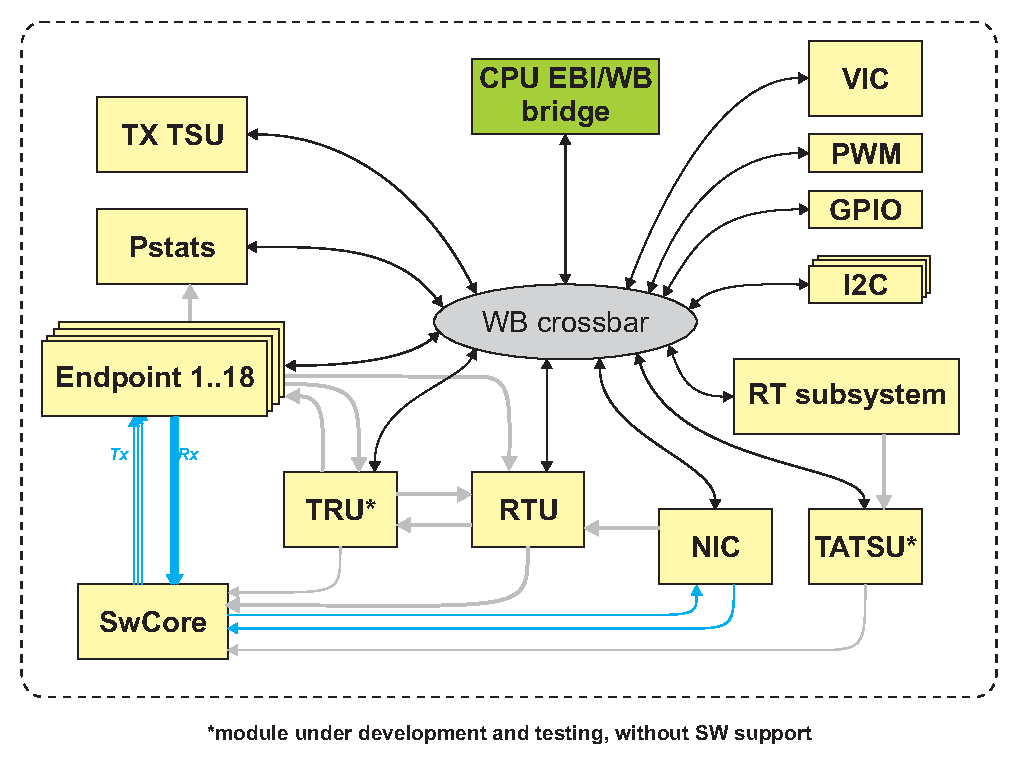
\includegraphics[width=\textwidth]{switch/switch_hdl_v4.0.ps}
    \caption{Top HDL design of the WR Switch}
    \label{fig:switch_top}
  \end{center}
\end{figure}

\begin{table}
  \begin{center}
  \begin{tabular}{|l|l|}
    \hline
    module name & base address\\
    \hline \hline
    Real-Time subsystem & 0x00000\\
    Network Interface Controller (NIC) & 0x20000\\
    Endpoint fanout & 0x30000\\
    Vectored Interrupt Controller (VIC) & 0x50000\\
    Tx Timestamping Unit (TX TSU) & 0x51000\\
    GPIO port (GPIO)  & 0x53000\\
    $I^2C$ master (I2C0, I2C1, Sensors\_I2C) & 0x54000\\
    PWM Controller & 0x55000\\
    Topology Resolution Unit (TRU) & 0x56000\\
    Time-Aware Traffic Shapper Unit (TATSU) & 0x57000\\
    Per-port Statistics (Pstats) & 0x58000\\
    Hardware Info Unit (HWIU) & 0x59000\\
    Routing Table Unit (RTU) & 0x60000\\
    \hline
  \end{tabular}
  \caption{Wishbone base addresses of modules inside WR Switch HDL}
  \label{tab:gov:wb_base}
  \end{center}
\end{table}

\section{Modules description}
\subsection{Real-Time Subsystem (RT subsystem)}

Contains modules responsible for the timekeeping. The components are internally connected
through WB crossbar (fig. \ref{fig:rts:hdl}) and controlled from Lattice Mico 32
and main CPU (through primary WB crossbar in the top design). Table
\ref{tab:rts:wb_base} contains Wishbone base address of each module inside the
Real-Time Subsystem.

\begin{figure}[ht]
  \begin{center}
    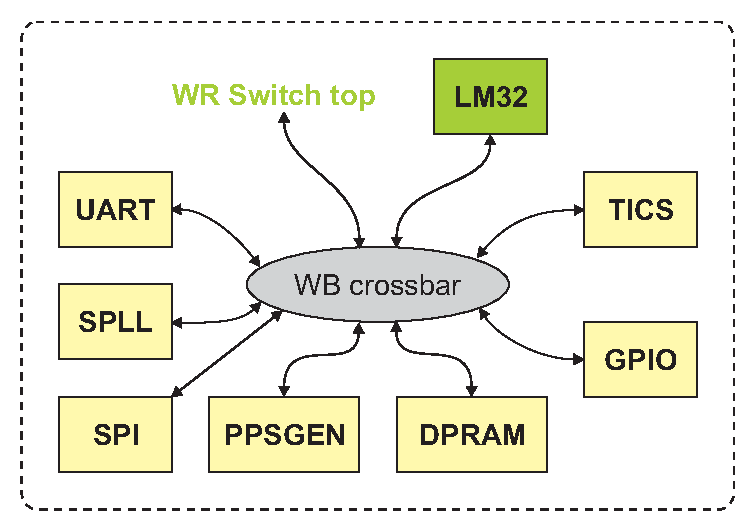
\includegraphics[width=.8\textwidth]{switch/rt_sub.pdf}
    \caption{Internal layout of Real-Time Subsystem block}
    \label{fig:rts:hdl}
  \end{center}
\end{figure}

\begin{table}[ht]
  \begin{center}
  \begin{tabular}{|l|l|}
    \hline
    module name & base address\\
    \hline \hline
    Dual-port RAM & 0x00000\\
    debug UART & 0x10000\\
    Soft-PLL & 0x10100\\
    SPI & 0x10200\\
    GPIO & 0x10300\\
    Timer block (TICS) & 0x10400\\
    1-PPS generator (PPSGEN) & 0x10500\\
    \hline
  \end{tabular}
  \caption{Wishbone base addresses of modules inside the Real-Time Subsystem}
  \label{tab:rts:wb_base}
  \end{center}
\end{table}

\subsubsection{LatticeMico32 (LM32)}
\noindent {\bf Description:}

Soft-core processor executing software implementation of PLLs (with
\emph{Soft-PLL} module).\\

\noindent{\bf Wishbone interface:}

\emph{LM32} is a Wishbone Master, does not have any WB configuration registers.

\subsubsection{Dual-port RAM (DPRAM)}
\noindent {\bf Description:}

Instruction and data memory for \emph{LM32} soft-core processor
controlling \emph{Soft-PLL}. It has to be programmed with \emph{LM32} binary
from the main CPU when the WR Switch boots.

\subsubsection{Debug UART}
\noindent {\bf Description:}

UART driven by \emph{LM32}, outputs debug information from Software PLLs.\\

\noindent{\bf Wishbone interface:}

Only \emph{LM32} talks to this interface, WR Switch software does not access it.

\subsubsection{Soft-PLL (SPLL)}
\noindent {\bf Description:}

HDL part of Soft-PLL implementation. Controlled over Wishbone from \emph{LM32}
software.\\

\noindent{\bf Wishbone interface:}

Only \emph{LM32} talks to this interface, WR Switch software does not access it.

\subsubsection{SPI}
\noindent {\bf Description:}

Used by software running on \emph{LM32} to adjust the tunable oscillators (part
of SoftPLL implementation).\\

\noindent{\bf Wishbone interface:}

Only \emph{LM32} talks to this interface, WR Switch software does not access it.

\subsubsection{GPIO}
\noindent {\bf Description:}

Controls GPIO lines through Wishbone interface. All of the signals currently
used are output-only. They are mostly (besides GPIO2) driven from \emph{LM32}
software as part of SoftPLL algorithm implementation.

Signals controlled by the module:

\begin{center}
  \begin{tabular}{|l|l|l|p{8cm}|}
    \hline
    {\bf GPIO No.} & {\bf direction} & {\bf used by} & {\bf description}\\
    \hline
    \hline
    0 & output & \emph{LM32} & selects system clock for FPGA modules to be a startup clock (0) or the
    clock coming from from PLL (1) i.e. aligned to WR time\\
    1 & output & \emph{LM32} & resets AD9516 clock generator\\
    2 & output & \emph{WR Switch SW} & active high reset of \emph{LM32} softcore, used by
    the \emph{LM32} firmware loader while it is being stored to DPRAM\\
    3 & output & \emph{LM32} & active low reset of WR Switch peripherals (Endpoint,
    Switching Core, Topology Resolution Unit, GTX Ser/Des, Tx Timestamping Unit,
    GPIO port of top design, $I^2C$ master interfaces, Per-port Statistics)\\
    4 - 31 & && not used\\ %\multicolumn{3}{l|}{not used}\\
    \hline
  \end{tabular}
\end{center}

\noindent{\bf Wishbone interface:} section \ref{subsec:wbgen:gpio}.

\subsubsection{Timer block}
\noindent {\bf Description:}

Used by \emph{LM32} for counting time intervals independent from the local
timebase (being adjusted).\\

\noindent{\bf Wishbone interface:}

Only \emph{LM32} talks to this interface, WR Switch software does not access it.

\subsubsection{1-PPS generator}
\noindent {\bf Description:}

The module is responsible for generating and inputting 1-PPS signal. It
contains two timekeeping counters: \emph{cntr\_utc} and \emph{cntr\_nsec}. The
former keeps full seconds of the White Rabbit time, while the latter represents
fractional part of each second. \emph{cntr\_nsec} is clocked with 62.5 MHz
reference clock which means that its granularity is 16 ns. The 1-PPS pulse is
generated at the beginning of each second i.e. \emph{cntr\_nsec} equals to 0.

Wishbone registers of 1-PPS generator allow modifications of \emph{cntr\_utc}
and \emph{cntr\_nsec} counters. It can be performed in two ways: setting or
adjusting the time. The former simply stores new values to the counters when
requested. The adjustment is done by adding new values to the current state of
the counters (\emph{cntr\_utc}, \emph{cntr\_nsec}) at the beginning of a new second (when \emph{cntr\_nsec} is 0).\\

\noindent{\bf Wishbone interface:} section \ref{subsec:wbgen:ppsg}.

\subsection{Network Interface Controller}
\noindent {\bf Description:}

Module responsible for passing Ethernet frames between the Linux running
on the main ARM processor and 18 ports of WR Switch. It contains a \emph{frame
buffer} and two RAM blocks (\emph{TX descriptors memory}, \emph{RX descriptors
memory}) storing descriptors for frames received and frames to be sent.
Frame buffer stores all frames received from physical ports of WR Switch
(addressed to the main processor) and frames that main processor wants to send
to the ports of WR Switch. Each frame has an associated descriptor which
contains various information about its structure (figure \ref{fig:nic:tx_desc}
and figure \ref{fig:nic:rx_desc}).

When software running on main CPU wants to send an Ethernet frame, it has to
write it to the \emph{frame buffer} and then store the Tx descriptor describing
this frame into \emph{TX descriptors memory}. The other way round, first
software has to write an empty Rx descriptor (\emph{empty} bit set to \emph{1})
into the \emph{RX descriptors memory}. It has to describe the offset and length
of the area in the \emph{frame buffer} where \emph{NIC} can store received
frame. When a new frame is received \emph{NIC} will fill the Rx descriptor and
set \emph{empty} bit to \emph{0}.

When configured, \emph{Network Interface Controller} can also trigger three
different interrupts when:
\begin{itemize}
  \item a new Ethernet frame was received
  \item transmission of the frame is completed
  \item an error has occurred during the frame's transmission
\end{itemize} 
They are all combined into a single IRQ line connected to \emph{Vectored
Interrupt Controller} (sec.\ref{sec:vic}) so wishbone control register has to be
read to get the event which caused the interrupt.

\begin{figure}[ht]
  \begin{center}
    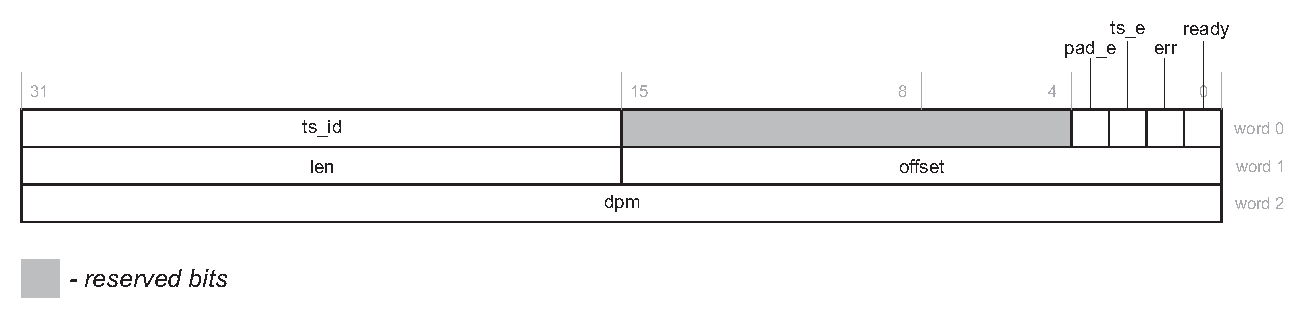
\includegraphics[width=\textwidth]{switch/nic_txdesc.pdf}
    \caption{Tx descriptor}
    \label{fig:nic:tx_desc}
  \end{center}
\end{figure}
\newpage
\begin{tabular}{l p{12cm}}
  \emph{ready} & if \emph{1}, whole descriptor is stored in memory, frame can be
  transmitted\\
  \emph{err} & if \emph{1}, an error has occurred during frame's
    transmission\\
  \emph{ts\_e} & if \emph{1}, request frame timestamping\\
  \emph{pad\_e} & if \emph{1}, frame is runt and requires padding\\
  \emph{ts\_id} & frame id, needed to associate Tx timestamp (from Tx
    Timestamping Unit) with appropriate frame\\
  \emph{offset} & offset of the frame inside \emph{frame buffer}\\
  \emph{len} & length of the frame\\
  \emph{dpm} & destination port mask, each bit set to \emph{1} will
    result in Ethernet frame sent from that physical port\\
\end{tabular}


\begin{figure}[ht]
  \begin{center}
    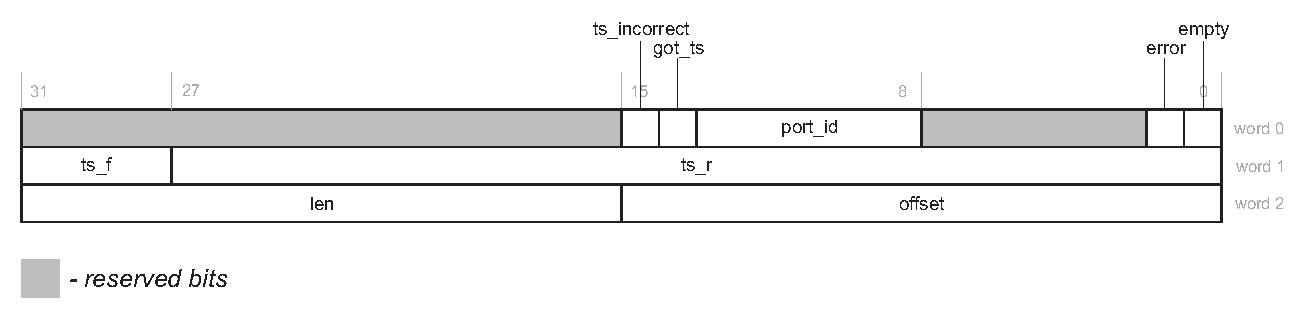
\includegraphics[width=\textwidth]{switch/nic_rxdesc.pdf}
    \caption{Rx descriptor}
    \label{fig:nic:rx_desc}
  \end{center}
\end{figure}
\begin{tabular}{l p{12cm}}
  \emph{empty} & if \emph{1}, descriptor is empty, and can be written by
  reception FSM\\
  \emph{error} & if \emph{1}, an error has occurred during the reception of the
  frame\\
  \emph{port\_id} & the ID of the physical port which has received the frame\\
  \emph{got\_ts} & if \emph{1}, received frame contains OOB data with Rx
  timestamp\\
  \emph{ts\_incorrect} & if \emph{1}, Rx timestamp may be incorrect (generated
  during the adjustment of time base)\\
  \emph{ts\_r} & Rx timestamp generated on the rising edge of the reference
  clock\\
  \emph{ts\_f} & least significant bits of the Rx timestamp generated on the
  falling edge of the reference clock\\
  \emph{offset} & offset of the frame inside \emph{frame buffer}\\
  \emph{len} & length of the allocated buffer for Rx frame (when \emph{empty}
  is \emph{1}) or length of the received frame (when \emph{empty} is \emph{0})
  received frame when
\end{tabular}

\vspace{12pt}
\noindent{\bf Wishbone interface:}

Wishbone interface of WR NIC contains two areas with different base addresses:\\

\begin{tabular}{l l}
  configuration registers & 0x20000\\
            frame buffer  & 0x28000\\
\end{tabular}

\vspace{12pt}
The description of configuration registers can be found in section
\ref{subsec:wbgen:nic}.

\subsection{Endpoint fanout}

The Endpoint fanout contains configurable amount of Endpoint
modules connected together with the Wishbone Crossbar.\\

Base Wishbone addresses of Endpoints:\\

\begin{tabular}{|l|l|}
  \hline
  module name & base address\\
  \hline \hline
  \emph{Endpoint 0} & 0x30000\\
  \emph{Endpoint 1} & 0x30400\\
  \emph{Endpoint 2} & 0x30800\\
  \emph{Endpoint 3} & 0x30c00\\
  \emph{Endpoint 4} & 0x31000\\
                ... & ...\\
  \emph{Endpoint n} & 0x30000 + n*0x400\\
  \hline
\end{tabular}\\

\noindent {\bf Description:}

Endpoint module implements Gigabit Ethernet MAC functionality and PCS for
Gigabit optical link. It sends and receives Ethernet frames from a physical link
and is able to generate precise Tx and Rx timestamps. It also has VLAN and Flow
Control (receiving Pause frames) support. 

Additionally it is able to inject frames required by the Topology Resolution
Unit (sec. \ref{sec:tru}) for hardware supported RSTP and generates events
counted by Per-port Statistics module (sec. \ref{sec:pstats}).

Endpoint contains also a programmable packet filter, which can classify
incoming Ethernet frames into 8 different classes.\\

\noindent{\bf Wishbone interface:} section \ref{subsec:wbgen:ep}.

\subsubsection{Programmable packet filter}
The description of the packet filter inside the
Endpoint module is taken from \emph{dev/ep\_pfilter.c} file stored in
White Rabbit PTP Core Software repository.\\

The classifier processes the incoming frame, and assigns it to one of 8 classes
(an 8-bit word, where each bit corresponds to a particular class) or eventually
drops it. Hardware implementation of the unit is a simple VLIW processor with 32
single-bit registers (0 - 31). The registers are organized as follows:
\begin{itemize}
  \item 0: don't touch (always 0)
  \item 1 - 22: general purpose registers
  \item 23: drop frame flag: if 1 at the end of the frame processing, the frame will be dropped.
  \item 24..31: packet class (class 0 = reg 24, class 7 = reg 31).
\end{itemize}

Program memory has 64 36-bit words. Packet filtering program is restarted every
time a new frame comes.
There are 5 possible instructions:

\begin{enumerate}
  \item \emph{CMP offset, value, mask, oper, Rd}:\\
    Rd = Rd oper ((((uint16\_t *)frame) [offset] \& mask) == value)
    
    \underline{Examples:}
    \begin{itemize}
      \item \emph{CMP 3, 0xcafe, 0xffff, MOV, Rd}\\
            will compare the 3rd word of the frame (bytes 6, 7) against 0xcafe
            and if the words are equal, 1 will be written to Rd register.
      \item \emph{CMP 4, 0xbabe, 0xffff, AND, Rd}\\
            will do the same with the 4th word and write to Rd its previous
            value ANDed with the result of the comparison. Effectively, Rd now
            will be 1 only if bytes [6..9] of the payload contain word
            0xcafebabe.
    
            Note that the mask value is nibble-granular. That means you can
            choose a particular set of nibbles within a word to be compared, but
            not an arbitrary set of bits (e.g. 0xf00f, 0xff00 and 0xf0f0 masks
            are ok, but 0x8001 is wrong.
    \end{itemize}

  \item \emph{BTST offset, bit\_number, oper, Rd}:\\
    Rd = Rd oper (((uint16\_t *)frame) [offset] \& (1$\ll$bit\_number) ? 1 : 0)

    \underline{Examples:}
    \begin{itemize}
      \item \emph{BTST 3, 10, MOV, 11}\\
            will write 1 to reg 11 if the 10th bit in the 3rd word of the frame 
            is set (and 0 if it's clear)
    \end{itemize}

  \item Logic opearations:
    \begin{itemize}
      \item \emph{LOGIC2 Rd, Ra, OPER Rb} - 2 argument logic (Rd = Ra OPER Rb). If the
            operation is MOV or NOT, Ra is taken as the source register.
      \item \emph{LOGIC3 Rd, Ra, OPER Rb, OPER2, Rc} - 3 argument logic Rd = (Ra
            OPER Rb) OPER2 Rc.
    \end{itemize}

  \item Miscellaneous:
    \begin{itemize}
      \item \emph{FIN} instruction terminates the program.
      \item \emph{NOP} executes a dummy instruction (LOGIC2 0, 0, AND, 0)
    \end{itemize}
\end{enumerate}

IMPORTANT:
\begin{itemize}
  \item the program counter is advanced each time a 16-bit words of the frame arrives.
  \item the CPU doesn't have any interlocks to simplify the HW, so you can't
    compare the 10th word when PC = 2. Max comparison offset is always equal to
    the address of the instruction.
  \item Code may contain up to 64 operations, but it must classify shorter frames faster than in
  32 instructions (there's no flow throttling)
\end{itemize}

\subsubsection{Injection engine}
The frame injection engine has to be programmed first with frames' templates
and after that sending (injecting) each template can be triggered from the TRU
module.

Storing frame templates is done through the \emph{VCR1} Wishbone register. Each
word written to this register is a concatenation of the offset value and the data
word (check section \ref{subsec:wbgen:ep}). Since the same block RAM is shared
by the Injection engine and VLAN unit, templates have to be stored starting with
the offset {\bf 512}. This buffer can store up to 8 templates each not longer
than 128 bytes.

Storing a frame's template requires splitting such frame into 2-byte words and
performing a set of writes into the \emph{VCR1} register (each time the offset
value has to be incremented). The format of data word is presented in figure
\ref{fig:ep:inject_data}:
\begin{figure}[ht]
  \begin{center}
    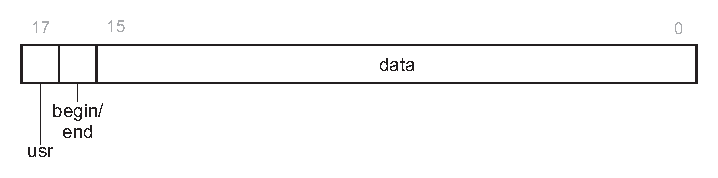
\includegraphics[width=.8\textwidth]{../../../../figures/switch/ep_inject.ps}
    \caption{Format of data word for programming the injection engine}
    \label{fig:ep:inject_data}
  \end{center}
\end{figure}

\begin{tabular}{l p{13cm}}
  \emph{data} & 2-byte chunk of the template\\
  \emph{begin/end} & if set to 1, the written word is first or last word of
    template's data\\
  \emph{usr} & if set to 1, this data word will be replaced by the value
    provided by the TRU module\\
\end{tabular}

\subsection{Vectored Interrupt Controller (VIC)}
\label{sec:vic}

\noindent {\bf Description:}

The module combines multiple interrupt lines from different modules inside the
WR Switch Gateware and outputs a single IRQ fed to the main CPU. It inputs up to 32
prioritized internal interrupts. The priorities of the interrupts are fixed: IRQ0 has
the highest priority while IRQ31 has the lowest priority. Currently 4 internal
interrupts are connected to \emph{VIC}:
\begin{center}
\begin{tabular}{|l|l|}
  \hline
  IRQ No. & source module\\
  \hline \hline
  0 & Network Interface Controller (\emph{NIC})\\
  1 & Tx Timestamping Unit (\emph{TS TSU})\\
  2 & Routing Table Unit (\emph{RTU})\\
  3 & Per-port Statistics (\emph{Pstats})\\
  4 - 31 & currently not used\\
  \hline
\end{tabular}
\end{center}

\vspace{12pt}
\noindent{\bf Wishbone interface:} section \ref{subsec:wbgen:VIC}.

\subsection{Tx Timestamping Unit (Tx TSU)}

\noindent {\bf Description:}

The module collects Tx timestamps for Ethernet frames sent through all 18
Endpoints available in WR Switch. Those timestamps are stored inside the FIFO
queue and can be fetched by the software running on the main CPU together with
the Frame ID (FID) and Port ID (PID). This additional information is used by
the CPU to associate the timestamp with appropriate frame that was sent through
\emph{NIC} and one (or multiple) of the Endpoints.

The module can also generate an interrupt (fed to VIC described in section
\ref{sec:vic}). It indicates that TxTSU stores at least one timestamp in its
FIFO.\\

\noindent{\bf Wishbone interface:} section \ref{subsec:wbgen:txtsu}.

\subsection{GPIO port}

\noindent {\bf Description:}

The module controls GPIO lines through Wishbone interface. The direction
(input/output) is set separately for each line.

Currently only one GPIO line driven from this module is used in WR Switch. It
selects whether the debug UART (from Real-Time Subsystem) or UART from the main CPU
will be available on a physical UART connector of the WR Switch.\\

\begin{center}
\begin{tabular}{|l|l|}
  \hline
  GPIO No. & description\\
  \hline \hline
  0 - 30 & not used\\
      31 & uart select\\
  \hline
\end{tabular}
\end{center}

\vspace{12pt}
\noindent{\bf Wishbone interface:} section \ref{subsec:wbgen:gpio}.

\subsection{$I^2C$ master}

There are three identical $I^2C$ masters:
\begin{itemize}
  \item \emph{I2C0}: drives $I^2C$ GPIO expansion chip for ports 16-17
    \footnote{Check the schematics of WR Switch miniBackplane for details what
    is driven by those GPIOs.}
  \item \emph{I2C1}: drives $I^2C$ GPIO expansion chip for ports 0-15
  \item \emph{Sensors I2C}: connected to the set of \emph{TMP100} digital
    thermometers
\end{itemize}

\noindent {\bf Description:}

$I^2C$ master as its name says, implements the master of $I^2C$ bus. Before any
byte transfer is performed it must have the prescale value, used to
generate SCL clock, set.

The module is capable of generating interrupt, but it is not used in the WR Switch
design.\\

\noindent{\bf Wishbone interface:} section \ref{subsec:wbgen:i2c}.

\subsection{PWM Controller}

\noindent {\bf Description:}

Pulse Width Modulation controller is used by the WR Switch software to adjust the
speed of two fans installed at the back of a WR Switch box. The module can drive
up to 8 PWM channels, but only two are currently used:

\begin{center}
  \begin{tabular}{|l|l|}
    \hline
    Channel No. & description\\
    \hline \hline
    0 & controlling the speed of the left fan\\
    1 & controlling the speed of the right fan\\
    \hline
  \end{tabular}
\end{center}

\vspace{12pt}
\noindent{\bf Wishbone interface:} section \ref{subsec:wbgen:spwm}.

\subsection{Topology Resolution Unit (TRU)}
\label{sec:tru}

\noindent {\bf Description:}

Module provides hardware support for topology resolution protocols implemented
in software (e.g. RSTP, LACP). It is still under testing and development so it
shouldn't be supported by the next official release of the WR Switch software.\\

\noindent{\bf Wishbone interface:} section \ref{subsec:wbgen:tru}.

\subsection{Time-Aware Traffic Shaper Unit (TATSU)}

\noindent {\bf Description:}

The module implements simple Time-Aware Traffic Shaper. It creates a time window
at a given (configured) moment (TAI + cycles) in a data stream transmitted
through WR Switch. In this window only selected output queues are allowed (the
others are blocked).

The module is still under testing and development so it
shouldn't be supported by the next official release of WR Switch Software.\\

\noindent{\bf Wishbone interface:} section \ref{subsec:wbgen:tatsu}.

\subsection{Per-port Statistics (Pstats)}
\label{sec:pstats}
\noindent {\bf Description:}

The module provides per-port statistics of the events presented in the table:\\

\noindent
\resizebox{\textwidth}{!}{
\begin{tabular}{|p{1cm}|c|c|p{9cm}|}
  \hline
  Event no. & name & source & description\\
  \hline \hline
  0 & \texttt{tx\_underrun} & \emph{Endpoint} & TX FIFO in PCS underrun\\
  1 & \texttt{rx\_overrun} & \emph{Endpoint} & RX FIFO in PCS overrun\\
  2 & \texttt{rx\_invalid\_code} & \emph{Endpoint} & received invalid 8B10B code\\
  3 & \texttt{rx\_sync\_lost} & \emph{Endpoint} & link synchronization lost\\
  4 & \texttt{rx\_pause} & \emph{Endpoint} & received pause frame\\
  5 & \texttt{rx\_pfilter\_drop} & \emph{Endpoint} & received frame dropped by Packet Filter\\
  6 & \texttt{rx\_pcs\_err} & \emph{Endpoint} & some error has occurred during frame reception (e.g.
  invalid code, fifo overrun, wrong frame termination, etc.)\\
  7 & \texttt{rx\_giant} & \emph{Endpoint} & received \emph{giant} frame (bigger than Maximum Receive
  Unit\\
  8 & \texttt{rx\_runt} & \emph{Endpoint} & received \emph{runt} frame (smaller than 64 bytes)\\
  9 & \texttt{rx\_crc\_err} & \emph{Endpoint} & CRC of the received frame does not match\\
 10 & \texttt{rx\_pclass(0)} & \emph{Endpoint} & RX frame got assigned to class 0 by Packet Filter\\
... & \texttt{...} & ... & ...\\
 17 & \texttt{rx\_pclass(7)} & \emph{Endpoint} & RX frame got assigned to class 7 by Packet Filter\\
 18 & \texttt{tx\_frame} & \emph{Endpoint} & frame was transmitted\\
 19 & \texttt{rx\_frame} & \emph{Endpoint} & frame was received\\
 20 & \texttt{req\_valid} & \emph{RTU} & got valid RTU request\\
 21 & \texttt{rsp\_valid} & \emph{RTU} & outputting valid RTU response\\
 22 & \texttt{rsp\_drop} & \emph{RTU} & frame dropped\\
 23 & \texttt{fm\_hp\_frame} & \emph{RTU} & got high priority frame\\
 24 & \texttt{fm\_fast\_fwd} & \emph{RTU} & fast forward frame (depending on RTU
  configuration, this can be broadcast frames, PTP frames, etc.)\\
 25 & \texttt{fm\_non\_fwd} & \emph{RTU} & don't forward frame (recognized
  link-limited frame, e.g. BPDU)\\
 26 & \emph{reserved} & \emph{RTU} & \\
 27 & \emph{reserved} & \emph{RTU} & \\
 \hline
\end{tabular}
}\\

Each event on each port has a separate 16-bit counter associated. It stores the
number of occurrence of the event. To be able to handle the bust of events from
a Gigabit Ethernet link, each counter is divided into two 8-bit halves creating
two layers of counting (L1, L2). Counters are aligned in those layers such a way
that each 32-bit word in memory stores the values of 4 counters:\\

\begin{tabular}{p{0.5cm}|p{2.5cm}|p{2.5cm}|p{2.5cm}|p{2.5cm}|}
  & {\scriptsize 31} \hfill {\scriptsize 24} & {\scriptsize 23} \hfill {\scriptsize 16} & 
  {\scriptsize 15} \hfill {\scriptsize 8} & {\scriptsize 7} \hfill {\scriptsize 0}\\
  \cline{2-5}
  L1 & \cellcolor{gray!25}CNTR3[7:0] & \cellcolor{gray!25}CNTR2[7:0] & 
  \cellcolor{gray!25}CNTR1[7:0] & \cellcolor{gray!25}CNTR0[7:0]\\
  \cline{2-5}
  L2 & \cellcolor{gray!25}CNTR3[15:8] & \cellcolor{gray!25}CNTR2[15:8] & 
  \cellcolor{gray!25}CNTR1[15:8] & \cellcolor{gray!25}CNTR0[15:8]\\
  \cline{2-5}
\end{tabular}\\

Therefore, one read operation from \emph{Pstats} module returns two 32-bit words
(L1, L2) from which user can extract the state of four subsequent counters.

The module generates an interrupt when any of the 16-bit counters on any of the
ports has overflown. After that \emph{EIC\_ISR} register indicates per-port IRQ,
and based on its content user can read per-port IRQ state using \emph{CR}
Wishbone register.\\

\noindent{\bf Wishbone interface:} section \ref{subsec:wbgen:pstats}.

\subsection{Hardware Info Unit (HWIU)}
\label{sec:hwiu}
\noindent {\bf Description:}

The module provides various information about the gateware build and can be also
used for debugging.

\begin{center}
  \begin{tabular}{|p{1.5cm}|p{9cm}|}
    \hline
    Reg No. & description\\
    \hline \hline
    0 & HWIU info structure\\
    1 & gateware build date (e.g. \emph{0C020E01})\\
    2 & commit hash of \emph{wr-switch-hdl} repository\\
    3 & commit hash of \emph{general-cores} repository\\
    4 & commit hash of \emph{wr-cores} repository\\
  ... & debug registers exporting values from various hdl modules, check hdl
    code for their meaning\\
    \hline
  \end{tabular}
\end{center}

HWIU info structure provides information about gateware details exported in HWIU
registers:

\begin{center}
  \begin{tabular}{|p{1.5cm}|p{9cm}|}
    \hline
    bit range & description\\
    \hline \hline
    31 - 24 & info structure version (currently \emph{1})\\
    23 - 16 & how many subsequent registers contain info about the gateware
    (currently \emph{4})\\
    15 -  8 & gateware major version (\emph{4})\\
     7 -  0 & gateware minor version (\emph{0})\\
    \hline
  \end{tabular}
\end{center}

Gateware build date is a 32-bit value which is a concatenation of day, month,
year and build number (if there are more then one build per day):

\begin{center}
  \begin{tabular}{|p{1.5cm}|p{9cm}|}
    \hline
    bit range & description\\
    \hline \hline
    31 - 24 & day of the build\\
    23 - 16 & month of the build\\
    15 -  8 & two digits of year of the build (e.g. for 2014 register stores \emph{14})\\
     7 -  0 & build number\\
    \hline
  \end{tabular}
\end{center}

\noindent{\bf Wishbone interface:} section \ref{subsec:wbgen:pstats}.

\subsection{Routing Table Unit (RTU)}

\noindent {\bf Description:}

RTU is responsible for making the decisions where (to which port or ports of the
Switch) each frame received from any of the ports has to be
forwarded. The decision is made based on the information from:
\begin{itemize}
  \item VLAN table: storing information about the VLAN configuration. Each entry
    contains a mask describing which physical ports belong to the VLAN (each bit
    set to \emph{1} means the port belongs to VLAN), index of VLAN group (FID)
    to which the VLAN belongs to, VLAN-assigned priority and also two additional
    bits, one saying that all frames belonging to the VLAN should be dropped and
    the other saying that every frame belonging to the VLAN should have its
    priority replaced with VLAN priority
  \item Hash table (HTAB): stores dynamic (the result of learning process) and
    static entries describing the presence of MAC addresses on physical ports of
    the Switch (i.e. MAC addresses of the devices connected to each physical
    port of the Switch)
  \item Topology Resolution Unit: responsible for dynamic network topology
    reconfiguration, more detailed description in section \ref{sec:tru}.
\end{itemize}

The Hash Table contains a set of MAC entries of the structure presented in the
table:\\

\noindent
\resizebox{\textwidth}{!}{
\begin{tabular}{|>{\centering\arraybackslash}p{1cm}|c|c|p{3cm}|p{8cm}|}
  \hline
  {\bf word no.} & {\bf offset} & {\bf length} & {\bf name} & {\bf description}\\
  \hline \hline
  \multirow{9}{*}{0} & 0 & 1 & \texttt{valid} & if 1, the entry contains valid data\\
  \cline{2-5}
  & 1 & 1 & \multicolumn{2}{l|}{\emph{reserved}}\\
  \cline{2-5}
  & 2 & 1 & \texttt{is\_bpdu} & if 1, accept frame even if the port is disabled in RTU
  configuration\\
  \cline{2-5}
  & 3 & 1 & \texttt{go\_to\_cam} & obsolete, will be removed or replaced\\
  \cline{2-5}
  & 4 & 8 & \texttt{fid} & Filtering Database ID which was used to generate the address
  (hash) of the entry\\
  \cline{2-5}
  & 12 & 4 & \multicolumn{2}{l|}{\emph{reserved}}\\
  \cline{2-5}
  & 16 & 16 & \texttt{mac[47:32]} & MAC address (high part)\\
  \hline \hline
  1 & 0 & 32 & \texttt{mac[31:0]} & MAC address (low part)\\
  \hline \hline
  \multirow{18}{*}{2} & 0 & 16 & \texttt{cam\_addr} & obsolete, will be removed or replaced\\
  \cline{2-5}
  & 16 & 1 & \texttt{has\_prio\_src} & validates prio\_src and prio\_override\_src
  fields\\
  \cline{2-5}
  & 17 & 3 & \texttt{prio\_src} & priority of the frame having source MAC matching with
  MAC of this entry\\
  \cline{2-5}
  & 20 & 1 & \texttt{prio\_ \linebreak override\_src} & override frame's priority with
  \emph{prio\_src} when its SMAC matches MAC of this entry\\
  \cline{2-5}
  & 21 & 1 & \texttt{drop\_when\_src} & drop frame when its SMAC matches MAC of this
  entry\\
  \cline{2-5}
  & 22 & 1 & \texttt{drop\_when\_ \linebreak unmatched\_ \linebreak src\_ports} & drop the frame when it comes
  from source port which does not belong to port\_mask\_src\\
  \cline{2-5}
  & 23 & 1 & \texttt{has\_prio\_dst} & validates prio\_dst and prio\_override\_dst\\
  \cline{2-5}
  & 24 & 3 & \texttt{prio\_dst} & priority of the frame having DMAC matching with MAC 
  of this entry\\
  \cline{2-5}
  & 27 & 1 & \texttt{prio\_ \linebreak override\_dst} & override frame's priority with
  \emph{prio\_dst} when its DMAC matches MAC of this entry\\
  \cline{2-5}
  & 28 & 1 & \texttt{drop\_when\_dst} & drop frame if its DMAC matches MAC of this
  entry\\
  \hline \hline
  \multirow{10}{*}{3} & 0 & 16 & \texttt{port\_mask\_ \linebreak src[15:0]} &
  low part of the port mask for SMAC, bit set
  to 1 indicates that frame with SMAC matching MAC of this entry can be
  forwarded from that port/ports. Ports having their bits set to 0 shall drop
  the frame\\
  \cline{2-5}
  & 16 & 16 & \texttt{port\_mask\_ \linebreak dst[15:0]} & low part of the port mask for DMAC, bit set
  to 1 indicates to which physical ports the frame with DMAC matching MAC of
  this entry shall be forwarded\\
  \hline \hline
  \multirow{4}{*}{4} & 0 & 16 & \texttt{port\_mask\_ \linebreak src[31:16]} &
  high part of the port mask for SMAC\\
  \cline{2-5}
  & 16 & 16 & \texttt{port\_mask\_ \linebreak dst[31:16]} & high part of the port mask for DMAC\\
  \hline
\end{tabular}
}

\vspace{12pt}
HTAB is organized in buckets. Each bucket stores five words of MAC entry
described in the table above. The bucket is addressed with the hash value
calculated from the FID and MAC address of the MAC entry it stores. This hash is
a CRC generated using one of the supported polynomials (\emph{POLY\_VAL} of GCR
Wishbone register). Since different MACs and FIDs can result in the same hash
value, each of the hash is associated with four buckets. If it turns out that
first bucket already stores a valid MAC entry, next one is checked. A new MAC
entry is then written to first free (not already used) bucket.

HTAB is written by the switch software and can contain both static entries
required by the configuration of the Switch and dynamic entries resulting from
learning process implemented in software. Write-only access to HTAB is provided
through MFIFO Wishbone registers (\emph{MFIFO\_R0}, \emph{MFIFO\_R1} and
\emph{MFIFO\_CSR}). The address of this memory has the structure presented in
figure \ref{fig:rtu:htab_adr}.

\begin{figure}[ht]
  \begin{center}
    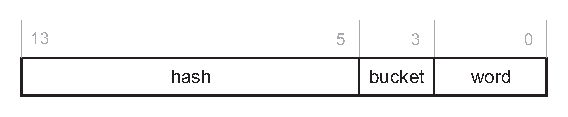
\includegraphics[width=.7\textwidth]{switch/rtu_mfifo_adr.ps}
  \end{center}
  \caption{Structure of HTAB address}
  \label{fig:rtu:htab_adr}
\end{figure}

To write a new MAC entry to HTAB first you have to write an address where the
first word of MAC entry will be written (least significant three bits -
\emph{word} - of the HTAB address equal 0) and then continue writing word by
word a complete entry:

\begin{tabular}{c|l}
  {\bf register} & {\bf value}\\
  \hline
  \texttt{MFIFO\_R0} & \emph{0x01}\\
  \texttt{MFIFO\_R1} & $<$HTAB address$>$\\
  \texttt{MFIFO\_R0} & \emph{0x00}\\
  \texttt{MFIFO\_R1} & $<$word 0$>$\\
  \texttt{MFIFO\_R1} & $<$word 1$>$\\
  \texttt{MFIFO\_R1} & $<$word 2$>$\\
  \texttt{MFIFO\_R1} & $<$word 3$>$\\
  \texttt{MFIFO\_R1} & $<$word 4$>$\\
\end{tabular}\\

The dynamic entries in HTAB should be created by learning mechanism based on the
information got from HDL through UFIFO (when learning on a port is enabled). RTU
module is capable of generating an interrupt when UFIFO is not empty i.e. it
stores at least one learning request. The UFIFO provides basic information
about the unrecognized frame: source MAC, destination MAC, optionally VLAN Id
and priority.\\

The RTU contains also the memory called ARAM which stores an aging bitmap. Each
bit corresponds to one MAC entry in HTAB and, when set to \emph{1}, indicates
that the MAC entry has been matched with the source MAC of the forwarded frame. The
memory is addressed in a similar way as HTAB, but since here each bit
corresponds to one MAC entry and each word is 32-bits long, the word in ARAM
is addressed with address from figure \ref{fig:rtu:htab_adr} shifted 8 bits to
the right (i.e. hash[8..3]). Three least significant bits of hash value
concatenated with the bucket number are used to find an appropriate bit in the word
read from the ARAM.\\

Besides the basic functionality described above, RTU has two main extensions:
\begin{itemize}
  \item {\bf port mirroring}: allows the ingress or egress traffic from selected
    port to be retransmitted on one or multiple other ports configured with
    appropriate mask
  \item {\bf Fast Match mechanism}: provides quick (23 clock cycles in worst case)
    routing response for selected types of frames
\end{itemize}

Fast Match can generate routing responses for (if appropriate bits are set in
\emph{RX\_CTR} control register):
\begin{itemize}
  \item broadcast frames: DMAC is FF:FF:FF:FF:FF:FF
  \item PTP frames: DMAC is 01:1B:19:00:00:00
  \item Link-Limited frames: DMAC in range from 01:80:C2:00:00:00 to
    01:80:C2:00:00:0F
  \item High Priority frames: which have priority included in the
    \emph{PRIO\_MASK} of \emph{RX\_CTR} register
  \item Any frame that has its DMAC in configured range of MAC addresses or DMAC
    equal to single configured MAC
\end{itemize}

\noindent{\bf Wishbone interface:} section \ref{subsec:wbgen:rtu}\\


\newpage
\section{Wishbone configuration interfaces}
\subsection{WR Switch PPS generator and RTC}
\label{subsec:wbgen:ppsg}
Unit generating PPS signals and acting as a UTC real-time clock
\subsubsection{Memory map summary}
\rowcolors{2}{gray!25}{white}
\resizebox{\textwidth}{!}{
\begin{tabular}{|l|l|l|l|l|}
\rowcolor{RoyalPurple}
\color{white} SW Offset & \color{white} Type & \color{white} Name &
\color{white} HW prefix & \color{white} C prefix\\
0x0& REG & Control Register & ppsg\_cr & CR\\
0x4& REG & Nanosecond counter register & ppsg\_cntr\_nsec & CNTR\_NSEC\\
0x8& REG & UTC Counter register (least-significant part) & ppsg\_cntr\_utclo & CNTR\_UTCLO\\
0xc& REG & UTC Counter register (most-significant part) & ppsg\_cntr\_utchi & CNTR\_UTCHI\\
0x10& REG & Nanosecond adjustment register & ppsg\_adj\_nsec & ADJ\_NSEC\\
0x14& REG & UTC Adjustment register (least-significant part) & ppsg\_adj\_utclo & ADJ\_UTCLO\\
0x18& REG & UTC Adjustment register (most-significant part) & ppsg\_adj\_utchi & ADJ\_UTCHI\\
0x1c& REG & External sync control register & ppsg\_escr & ESCR\\
\hline
\end{tabular}
}

\subsubsection{Register description}
\paragraph*{Control Register}\vspace{12pt}

\rowcolors{1}{white}{white}
\begin{tabular}{l l }
{\bf HW prefix:}  & ppsg\_cr\\
{\bf HW address:}  & 0x0\\
{\bf SW prefix:}  & CR\\
{\bf SW offset:}  & 0x0\\
\end{tabular}


\vspace{12pt}
\noindent
\resizebox{\textwidth}{!}{
\begin{tabular}{>{\centering\arraybackslash}p{1.5cm} >{\centering\arraybackslash}p{1.5cm} >{\centering\arraybackslash}p{1.5cm} >{\centering\arraybackslash}p{1.5cm} >{\centering\arraybackslash}p{1.5cm} >{\centering\arraybackslash}p{1.5cm} >{\centering\arraybackslash}p{1.5cm} >{\centering\arraybackslash}p{1.5cm} }
31 & 30 & 29 & 28 & 27 & 26 & 25 & 24\\
\hline
\multicolumn{8}{|c|}{\cellcolor{RoyalPurple!25}PWIDTH[27:20]}\\
\hline
23 & 22 & 21 & 20 & 19 & 18 & 17 & 16\\
\hline
\multicolumn{8}{|c|}{\cellcolor{RoyalPurple!25}PWIDTH[19:12]}\\
\hline
15 & 14 & 13 & 12 & 11 & 10 & 9 & 8\\
\hline
\multicolumn{8}{|c|}{\cellcolor{RoyalPurple!25}PWIDTH[11:4]}\\
\hline
7 & 6 & 5 & 4 & 3 & 2 & 1 & 0\\
\hline
\multicolumn{4}{|c|}{\cellcolor{RoyalPurple!25}PWIDTH[3:0]} & \multicolumn{1}{|c|}{\cellcolor{RoyalPurple!25}CNT\_SET} & \multicolumn{1}{|c|}{\cellcolor{RoyalPurple!25}CNT\_ADJ} & \multicolumn{1}{|c|}{\cellcolor{RoyalPurple!25}CNT\_EN} & \multicolumn{1}{|c|}{\cellcolor{RoyalPurple!25}CNT\_RST}\\
\hline
\end{tabular}
}

\begin{itemize}
\item \begin{small}
{\bf 
CNT\_RST
} [\emph{write-only}]: Reset counter
\\
write 1: resets the counter\\                				write 0: no effect
\end{small}
\item \begin{small}
{\bf 
CNT\_EN
} [\emph{read/write}]: Enable counter
\\
1: PPS counter is enabled
\end{small}
\item \begin{small}
{\bf 
CNT\_ADJ
} [\emph{read/write}]: Adjust offset
\\
write 1: Starts adjusting PPS/UTC offsets by adding the values taken from ADJ\_NSEC, ADJ\_UTCLO, ADJ\_UTCHI registers to the current PPS counter value. These registers need to be programmed prior to update.\\				                write 0: no effect\\				 read 0: adjustment operation is done\\				 read 1: adjustment operation is in progress
\end{small}
\item \begin{small}
{\bf 
CNT\_SET
} [\emph{write-only}]: Set time
\\
write 1: Sets the UTC/PPS counter to values taken from ADJ\_NSEC, ADJ\_UTCLO, ADJ\_UTCHI registers
\end{small}
\item \begin{small}
{\bf 
PWIDTH
} [\emph{read/write}]: PPS Pulse width
\\
Width of generated PPS pulses in 62.5 MHz refernce clock cycles
\end{small}
\end{itemize}
\paragraph*{Nanosecond counter register}\vspace{12pt}

\rowcolors{1}{white}{white}
\begin{tabular}{l l }
{\bf HW prefix:}  & ppsg\_cntr\_nsec\\
{\bf HW address:}  & 0x1\\
{\bf SW prefix:}  & CNTR\_NSEC\\
{\bf SW offset:}  & 0x4\\
\end{tabular}

\vspace{12pt}
Nanosecond part of current time, expressed as number of 62.5 MHz reference clock cycles

\vspace{12pt}
\noindent
\resizebox{\textwidth}{!}{
\begin{tabular}{>{\centering\arraybackslash}p{1.5cm} >{\centering\arraybackslash}p{1.5cm} >{\centering\arraybackslash}p{1.5cm} >{\centering\arraybackslash}p{1.5cm} >{\centering\arraybackslash}p{1.5cm} >{\centering\arraybackslash}p{1.5cm} >{\centering\arraybackslash}p{1.5cm} >{\centering\arraybackslash}p{1.5cm} }
31 & 30 & 29 & 28 & 27 & 26 & 25 & 24\\
\hline
\multicolumn{1}{|c}{-} & - & - & - & \multicolumn{4}{|c|}{\cellcolor{RoyalPurple!25}CNTR\_NSEC[27:24]}\\
\hline
23 & 22 & 21 & 20 & 19 & 18 & 17 & 16\\
\hline
\multicolumn{8}{|c|}{\cellcolor{RoyalPurple!25}CNTR\_NSEC[23:16]}\\
\hline
15 & 14 & 13 & 12 & 11 & 10 & 9 & 8\\
\hline
\multicolumn{8}{|c|}{\cellcolor{RoyalPurple!25}CNTR\_NSEC[15:8]}\\
\hline
7 & 6 & 5 & 4 & 3 & 2 & 1 & 0\\
\hline
\multicolumn{8}{|c|}{\cellcolor{RoyalPurple!25}CNTR\_NSEC[7:0]}\\
\hline
\end{tabular}
}

\begin{itemize}
\item \begin{small}
{\bf 
CNTR\_NSEC
} [\emph{read-only}]: Nanosecond counter
\end{small}
\end{itemize}
\paragraph*{UTC Counter register (least-significant part)}\vspace{12pt}

\rowcolors{1}{white}{white}
\begin{tabular}{l l }
{\bf HW prefix:}  & ppsg\_cntr\_utclo\\
{\bf HW address:}  & 0x2\\
{\bf SW prefix:}  & CNTR\_UTCLO\\
{\bf SW offset:}  & 0x8\\
\end{tabular}

\vspace{12pt}
Lower 32 bits of current UTC time

\vspace{12pt}
\noindent
\resizebox{\textwidth}{!}{
\begin{tabular}{>{\centering\arraybackslash}p{1.5cm} >{\centering\arraybackslash}p{1.5cm} >{\centering\arraybackslash}p{1.5cm} >{\centering\arraybackslash}p{1.5cm} >{\centering\arraybackslash}p{1.5cm} >{\centering\arraybackslash}p{1.5cm} >{\centering\arraybackslash}p{1.5cm} >{\centering\arraybackslash}p{1.5cm} }
31 & 30 & 29 & 28 & 27 & 26 & 25 & 24\\
\hline
\multicolumn{8}{|c|}{\cellcolor{RoyalPurple!25}CNTR\_UTCLO[31:24]}\\
\hline
23 & 22 & 21 & 20 & 19 & 18 & 17 & 16\\
\hline
\multicolumn{8}{|c|}{\cellcolor{RoyalPurple!25}CNTR\_UTCLO[23:16]}\\
\hline
15 & 14 & 13 & 12 & 11 & 10 & 9 & 8\\
\hline
\multicolumn{8}{|c|}{\cellcolor{RoyalPurple!25}CNTR\_UTCLO[15:8]}\\
\hline
7 & 6 & 5 & 4 & 3 & 2 & 1 & 0\\
\hline
\multicolumn{8}{|c|}{\cellcolor{RoyalPurple!25}CNTR\_UTCLO[7:0]}\\
\hline
\end{tabular}
}

\begin{itemize}
\item \begin{small}
{\bf 
CNTR\_UTCLO
} [\emph{read-only}]: UTC Counter
\end{small}
\end{itemize}
\paragraph*{UTC Counter register (most-significant part)}\vspace{12pt}

\rowcolors{1}{white}{white}
\begin{tabular}{l l }
{\bf HW prefix:}  & ppsg\_cntr\_utchi\\
{\bf HW address:}  & 0x3\\
{\bf SW prefix:}  & CNTR\_UTCHI\\
{\bf SW offset:}  & 0xc\\
\end{tabular}

\vspace{12pt}
Highest 8 bits of current UTC time

\vspace{12pt}
\noindent
\resizebox{\textwidth}{!}{
\begin{tabular}{>{\centering\arraybackslash}p{1.5cm} >{\centering\arraybackslash}p{1.5cm} >{\centering\arraybackslash}p{1.5cm} >{\centering\arraybackslash}p{1.5cm} >{\centering\arraybackslash}p{1.5cm} >{\centering\arraybackslash}p{1.5cm} >{\centering\arraybackslash}p{1.5cm} >{\centering\arraybackslash}p{1.5cm} }
31 & 30 & 29 & 28 & 27 & 26 & 25 & 24\\
\hline
\multicolumn{1}{|c}{-} & - & - & - & - & - & - & \multicolumn{1}{c|}{-}\\
\hline
23 & 22 & 21 & 20 & 19 & 18 & 17 & 16\\
\hline
\multicolumn{1}{|c}{-} & - & - & - & - & - & - & \multicolumn{1}{c|}{-}\\
\hline
15 & 14 & 13 & 12 & 11 & 10 & 9 & 8\\
\hline
\multicolumn{1}{|c}{-} & - & - & - & - & - & - & \multicolumn{1}{c|}{-}\\
\hline
7 & 6 & 5 & 4 & 3 & 2 & 1 & 0\\
\hline
\multicolumn{8}{|c|}{\cellcolor{RoyalPurple!25}CNTR\_UTCHI[7:0]}\\
\hline
\end{tabular}
}

\begin{itemize}
\item \begin{small}
{\bf 
CNTR\_UTCHI
} [\emph{read-only}]: UTC Counter
\end{small}
\end{itemize}
\paragraph*{Nanosecond adjustment register}\vspace{12pt}

\rowcolors{1}{white}{white}
\begin{tabular}{l l }
{\bf HW prefix:}  & ppsg\_adj\_nsec\\
{\bf HW address:}  & 0x4\\
{\bf SW prefix:}  & ADJ\_NSEC\\
{\bf SW offset:}  & 0x10\\
\end{tabular}

\vspace{12pt}
Adjustment value for nanosecond counter

\vspace{12pt}
\noindent
\resizebox{\textwidth}{!}{
\begin{tabular}{>{\centering\arraybackslash}p{1.5cm} >{\centering\arraybackslash}p{1.5cm} >{\centering\arraybackslash}p{1.5cm} >{\centering\arraybackslash}p{1.5cm} >{\centering\arraybackslash}p{1.5cm} >{\centering\arraybackslash}p{1.5cm} >{\centering\arraybackslash}p{1.5cm} >{\centering\arraybackslash}p{1.5cm} }
31 & 30 & 29 & 28 & 27 & 26 & 25 & 24\\
\hline
\multicolumn{1}{|c}{-} & - & - & - & \multicolumn{4}{|c|}{\cellcolor{RoyalPurple!25}ADJ\_NSEC[27:24]}\\
\hline
23 & 22 & 21 & 20 & 19 & 18 & 17 & 16\\
\hline
\multicolumn{8}{|c|}{\cellcolor{RoyalPurple!25}ADJ\_NSEC[23:16]}\\
\hline
15 & 14 & 13 & 12 & 11 & 10 & 9 & 8\\
\hline
\multicolumn{8}{|c|}{\cellcolor{RoyalPurple!25}ADJ\_NSEC[15:8]}\\
\hline
7 & 6 & 5 & 4 & 3 & 2 & 1 & 0\\
\hline
\multicolumn{8}{|c|}{\cellcolor{RoyalPurple!25}ADJ\_NSEC[7:0]}\\
\hline
\end{tabular}
}

\begin{itemize}
\item \begin{small}
{\bf 
ADJ\_NSEC
} [\emph{write-only}]: Nanosecond adjustment
\end{small}
\end{itemize}
\paragraph*{UTC Adjustment register (least-significant part)}\vspace{12pt}

\rowcolors{1}{white}{white}
\begin{tabular}{l l }
{\bf HW prefix:}  & ppsg\_adj\_utclo\\
{\bf HW address:}  & 0x5\\
{\bf SW prefix:}  & ADJ\_UTCLO\\
{\bf SW offset:}  & 0x14\\
\end{tabular}

\vspace{12pt}
Lower 32 bits of adjustment value for UTC

\vspace{12pt}
\noindent
\resizebox{\textwidth}{!}{
\begin{tabular}{>{\centering\arraybackslash}p{1.5cm} >{\centering\arraybackslash}p{1.5cm} >{\centering\arraybackslash}p{1.5cm} >{\centering\arraybackslash}p{1.5cm} >{\centering\arraybackslash}p{1.5cm} >{\centering\arraybackslash}p{1.5cm} >{\centering\arraybackslash}p{1.5cm} >{\centering\arraybackslash}p{1.5cm} }
31 & 30 & 29 & 28 & 27 & 26 & 25 & 24\\
\hline
\multicolumn{8}{|c|}{\cellcolor{RoyalPurple!25}ADJ\_UTCLO[31:24]}\\
\hline
23 & 22 & 21 & 20 & 19 & 18 & 17 & 16\\
\hline
\multicolumn{8}{|c|}{\cellcolor{RoyalPurple!25}ADJ\_UTCLO[23:16]}\\
\hline
15 & 14 & 13 & 12 & 11 & 10 & 9 & 8\\
\hline
\multicolumn{8}{|c|}{\cellcolor{RoyalPurple!25}ADJ\_UTCLO[15:8]}\\
\hline
7 & 6 & 5 & 4 & 3 & 2 & 1 & 0\\
\hline
\multicolumn{8}{|c|}{\cellcolor{RoyalPurple!25}ADJ\_UTCLO[7:0]}\\
\hline
\end{tabular}
}

\begin{itemize}
\item \begin{small}
{\bf 
ADJ\_UTCLO
} [\emph{write-only}]: UTC Counter adjustment
\end{small}
\end{itemize}
\paragraph*{UTC Adjustment register (most-significant part)}\vspace{12pt}

\rowcolors{1}{white}{white}
\begin{tabular}{l l }
{\bf HW prefix:}  & ppsg\_adj\_utchi\\
{\bf HW address:}  & 0x6\\
{\bf SW prefix:}  & ADJ\_UTCHI\\
{\bf SW offset:}  & 0x18\\
\end{tabular}

\vspace{12pt}
Highest 8 bits of adjustment value for UTC

\vspace{12pt}
\noindent
\resizebox{\textwidth}{!}{
\begin{tabular}{>{\centering\arraybackslash}p{1.5cm} >{\centering\arraybackslash}p{1.5cm} >{\centering\arraybackslash}p{1.5cm} >{\centering\arraybackslash}p{1.5cm} >{\centering\arraybackslash}p{1.5cm} >{\centering\arraybackslash}p{1.5cm} >{\centering\arraybackslash}p{1.5cm} >{\centering\arraybackslash}p{1.5cm} }
31 & 30 & 29 & 28 & 27 & 26 & 25 & 24\\
\hline
\multicolumn{1}{|c}{-} & - & - & - & - & - & - & \multicolumn{1}{c|}{-}\\
\hline
23 & 22 & 21 & 20 & 19 & 18 & 17 & 16\\
\hline
\multicolumn{1}{|c}{-} & - & - & - & - & - & - & \multicolumn{1}{c|}{-}\\
\hline
15 & 14 & 13 & 12 & 11 & 10 & 9 & 8\\
\hline
\multicolumn{1}{|c}{-} & - & - & - & - & - & - & \multicolumn{1}{c|}{-}\\
\hline
7 & 6 & 5 & 4 & 3 & 2 & 1 & 0\\
\hline
\multicolumn{8}{|c|}{\cellcolor{RoyalPurple!25}ADJ\_UTCHI[7:0]}\\
\hline
\end{tabular}
}

\begin{itemize}
\item \begin{small}
{\bf 
ADJ\_UTCHI
} [\emph{write-only}]: UTC Counter adjustment
\end{small}
\end{itemize}
\paragraph*{External sync control register}\vspace{12pt}

\rowcolors{1}{white}{white}
\begin{tabular}{l l }
{\bf HW prefix:}  & ppsg\_escr\\
{\bf HW address:}  & 0x7\\
{\bf SW prefix:}  & ESCR\\
{\bf SW offset:}  & 0x1c\\
\end{tabular}


\vspace{12pt}
\noindent
\resizebox{\textwidth}{!}{
\begin{tabular}{>{\centering\arraybackslash}p{1.5cm} >{\centering\arraybackslash}p{1.5cm} >{\centering\arraybackslash}p{1.5cm} >{\centering\arraybackslash}p{1.5cm} >{\centering\arraybackslash}p{1.5cm} >{\centering\arraybackslash}p{1.5cm} >{\centering\arraybackslash}p{1.5cm} >{\centering\arraybackslash}p{1.5cm} }
31 & 30 & 29 & 28 & 27 & 26 & 25 & 24\\
\hline
\multicolumn{1}{|c}{-} & - & - & - & - & - & - & \multicolumn{1}{c|}{-}\\
\hline
23 & 22 & 21 & 20 & 19 & 18 & 17 & 16\\
\hline
\multicolumn{1}{|c}{-} & - & - & - & - & - & - & \multicolumn{1}{c|}{-}\\
\hline
15 & 14 & 13 & 12 & 11 & 10 & 9 & 8\\
\hline
\multicolumn{1}{|c}{-} & - & - & - & - & - & - & \multicolumn{1}{c|}{-}\\
\hline
7 & 6 & 5 & 4 & 3 & 2 & 1 & 0\\
\hline
\multicolumn{1}{|c}{-} & - & - & - & - & \multicolumn{1}{|c|}{\cellcolor{RoyalPurple!25}TM\_VALID} & \multicolumn{1}{|c|}{\cellcolor{RoyalPurple!25}PPS\_VALID} & \multicolumn{1}{|c|}{\cellcolor{RoyalPurple!25}SYNC}\\
\hline
\end{tabular}
}

\begin{itemize}
\item \begin{small}
{\bf 
SYNC
} [\emph{read/write}]: Sync to external PPS input
\\
write 1: Waits until a pulse on external PPS input arrives and re-synchronizes the PPS counter to it\\				 write 0: no effect\\				 read 1: external synchronization done\\				 read 0: external synchronization in progress
\end{small}
\item \begin{small}
{\bf 
PPS\_VALID
} [\emph{read/write}]: PPS output valid
\\
write 1: PPS output provides reliable 1-PPS signal\\                        write 0: PPS output is invalid
\end{small}
\item \begin{small}
{\bf 
TM\_VALID
} [\emph{read/write}]: Timecode output(UTC+cycles) valid
\\
write 1: Timecode output provides valid time\\                        write 0: Timecode output does not provide valid time
\end{small}
\end{itemize}




\newpage
\subsection{White Rabbit Switch NIC's spec}
\label{subsec:wbgen:nic}
This NIC is in between the endpoints and the on-board Linux CPU of the White Rabbit Switch.
\subsubsection{Memory map summary}
\rowcolors{2}{gray!25}{white}
\resizebox{\textwidth}{!}{
\begin{tabular}{|l|l|l|l|l|}
\rowcolor{RoyalPurple}
\color{white} SW Offset & \color{white} Type & \color{white} Name &
\color{white} HW prefix & \color{white} C prefix\\
0x0& REG & NIC Control Register & nic\_cr & CR\\
0x4& REG & NIC Status Register & nic\_sr & SR\\
0x20& REG & Interrupt disable register & nic\_eic\_idr & EIC\_IDR\\
0x24& REG & Interrupt enable register & nic\_eic\_ier & EIC\_IER\\
0x28& REG & Interrupt mask register & nic\_eic\_imr & EIC\_IMR\\
0x2c& REG & Interrupt status register & nic\_eic\_isr & EIC\_ISR\\
0x80 - 0xfc& MEM & TX descriptors mem & nic\_dtx & DTX\\
0x100 - 0x17c& MEM & RX descriptors mem & nic\_drx & DRX\\
\hline
\end{tabular}
}

\subsubsection{Register description}
\paragraph*{NIC Control Register}\vspace{12pt}

\rowcolors{1}{white}{white}
\begin{tabular}{l l }
{\bf HW prefix:}  & nic\_cr\\
{\bf HW address:}  & 0x0\\
{\bf SW prefix:}  & CR\\
{\bf SW offset:}  & 0x0\\
\end{tabular}


\vspace{12pt}
\noindent
\resizebox{\textwidth}{!}{
\begin{tabular}{>{\centering\arraybackslash}p{1.5cm} >{\centering\arraybackslash}p{1.5cm} >{\centering\arraybackslash}p{1.5cm} >{\centering\arraybackslash}p{1.5cm} >{\centering\arraybackslash}p{1.5cm} >{\centering\arraybackslash}p{1.5cm} >{\centering\arraybackslash}p{1.5cm} >{\centering\arraybackslash}p{1.5cm} }
31 & 30 & 29 & 28 & 27 & 26 & 25 & 24\\
\hline
\multicolumn{1}{|c|}{\cellcolor{RoyalPurple!25}SW\_RST} & - & - & - & - & - & - & \multicolumn{1}{c|}{-}\\
\hline
23 & 22 & 21 & 20 & 19 & 18 & 17 & 16\\
\hline
\multicolumn{1}{|c}{-} & - & - & - & - & - & - & \multicolumn{1}{c|}{-}\\
\hline
15 & 14 & 13 & 12 & 11 & 10 & 9 & 8\\
\hline
\multicolumn{1}{|c}{-} & - & - & - & - & - & - & \multicolumn{1}{c|}{-}\\
\hline
7 & 6 & 5 & 4 & 3 & 2 & 1 & 0\\
\hline
\multicolumn{1}{|c}{-} & - & - & - & - & - & \multicolumn{1}{|c|}{\cellcolor{RoyalPurple!25}TX\_EN} & \multicolumn{1}{|c|}{\cellcolor{RoyalPurple!25}RX\_EN}\\
\hline
\end{tabular}
}

\begin{itemize}
\item \begin{small}
{\bf 
RX\_EN
} [\emph{read/write}]: Receive enable
\\
write 1: enables receiving path \\                        write 0: disables receiving path \\                        read 1: receiving path enabled \\                        read 0: receiving path disabled
\end{small}
\item \begin{small}
{\bf 
TX\_EN
} [\emph{read/write}]: Transmit enable
\\
Enables the NIC to transmit data. When reset, the internal transmit pointer points to the first entry in the TX descriptor pool \\                        write 1: enables transmitting path \\                        write 0: disables transmitting path \\                        read 1: transmitting path enabled \\                        read 0: transmitting path disabled
\end{small}
\item \begin{small}
{\bf 
SW\_RST
} [\emph{write-only}]: Software Reset
\\
write 1: reset the NIC, zero all registers and reset the state of the module \\                       write 0: no effect
\end{small}
\end{itemize}
\paragraph*{NIC Status Register}\vspace{12pt}

\rowcolors{1}{white}{white}
\begin{tabular}{l l }
{\bf HW prefix:}  & nic\_sr\\
{\bf HW address:}  & 0x1\\
{\bf SW prefix:}  & SR\\
{\bf SW offset:}  & 0x4\\
\end{tabular}


\vspace{12pt}
\noindent
\resizebox{\textwidth}{!}{
\begin{tabular}{>{\centering\arraybackslash}p{1.5cm} >{\centering\arraybackslash}p{1.5cm} >{\centering\arraybackslash}p{1.5cm} >{\centering\arraybackslash}p{1.5cm} >{\centering\arraybackslash}p{1.5cm} >{\centering\arraybackslash}p{1.5cm} >{\centering\arraybackslash}p{1.5cm} >{\centering\arraybackslash}p{1.5cm} }
31 & 30 & 29 & 28 & 27 & 26 & 25 & 24\\
\hline
\multicolumn{1}{|c}{-} & - & - & - & - & - & - & \multicolumn{1}{c|}{-}\\
\hline
23 & 22 & 21 & 20 & 19 & 18 & 17 & 16\\
\hline
\multicolumn{1}{|c}{-} & - & - & - & - & \multicolumn{3}{|c|}{\cellcolor{RoyalPurple!25}CUR\_RX\_DESC[2:0]}\\
\hline
15 & 14 & 13 & 12 & 11 & 10 & 9 & 8\\
\hline
\multicolumn{1}{|c}{-} & - & - & - & - & \multicolumn{3}{|c|}{\cellcolor{RoyalPurple!25}CUR\_TX\_DESC[2:0]}\\
\hline
7 & 6 & 5 & 4 & 3 & 2 & 1 & 0\\
\hline
\multicolumn{1}{|c}{-} & - & - & - & \multicolumn{1}{|c|}{\cellcolor{RoyalPurple!25}TX\_ERROR} & \multicolumn{1}{|c|}{\cellcolor{RoyalPurple!25}TX\_DONE} & \multicolumn{1}{|c|}{\cellcolor{RoyalPurple!25}REC} & \multicolumn{1}{|c|}{\cellcolor{RoyalPurple!25}BNA}\\
\hline
\end{tabular}
}

\begin{itemize}
\item \begin{small}
{\bf 
BNA
} [\emph{read-only}]: Buffer Not Available
\\
read 1: no buffers were available when receiving a packet.
\end{small}
\item \begin{small}
{\bf 
REC
} [\emph{read/write}]: Frame Received
\\
read 1: one or more frames have been received. \\                        read 0: there is no new frame received \\				                write 1: clear the flag \\                        write 0: no effect
\end{small}
\item \begin{small}
{\bf 
TX\_DONE
} [\emph{read/write}]: Transmission done
\\
read 1: All non-empty TX descriptors have been transmitted\\				                read 0: Transmission in progress\\				 write 1: Clears the flag\\				 write 0: No effect
\end{small}
\item \begin{small}
{\bf 
TX\_ERROR
} [\emph{read/write}]: Transmission error
\\
read 1: A TX error occured and the transmission was stopped. CUR\_TX\_DESC is pointing the TX descriptor for which the error occured\\				                read 0: No TX error\\				 write 1: Clears the flag\\				 write 0: No effect
\end{small}
\item \begin{small}
{\bf 
CUR\_TX\_DESC
} [\emph{read-only}]: Current TX descriptor
\\
Index of the currently handled TX descriptor
\end{small}
\item \begin{small}
{\bf 
CUR\_RX\_DESC
} [\emph{read-only}]: Current RX descriptor
\\
Index of the currently handled RX descriptor
\end{small}
\end{itemize}
\paragraph*{Interrupt disable register}\vspace{12pt}

\rowcolors{1}{white}{white}
\begin{tabular}{l l }
{\bf HW prefix:}  & nic\_eic\_idr\\
{\bf HW address:}  & 0x8\\
{\bf SW prefix:}  & EIC\_IDR\\
{\bf SW offset:}  & 0x20\\
\end{tabular}

\vspace{12pt}
Writing 1 disables handling of the interrupt associated with corresponding bit. Writin 0 has no effect.

\vspace{12pt}
\noindent
\resizebox{\textwidth}{!}{
\begin{tabular}{>{\centering\arraybackslash}p{1.5cm} >{\centering\arraybackslash}p{1.5cm} >{\centering\arraybackslash}p{1.5cm} >{\centering\arraybackslash}p{1.5cm} >{\centering\arraybackslash}p{1.5cm} >{\centering\arraybackslash}p{1.5cm} >{\centering\arraybackslash}p{1.5cm} >{\centering\arraybackslash}p{1.5cm} }
31 & 30 & 29 & 28 & 27 & 26 & 25 & 24\\
\hline
\multicolumn{1}{|c}{-} & - & - & - & - & - & - & \multicolumn{1}{c|}{-}\\
\hline
23 & 22 & 21 & 20 & 19 & 18 & 17 & 16\\
\hline
\multicolumn{1}{|c}{-} & - & - & - & - & - & - & \multicolumn{1}{c|}{-}\\
\hline
15 & 14 & 13 & 12 & 11 & 10 & 9 & 8\\
\hline
\multicolumn{1}{|c}{-} & - & - & - & - & - & - & \multicolumn{1}{c|}{-}\\
\hline
7 & 6 & 5 & 4 & 3 & 2 & 1 & 0\\
\hline
\multicolumn{1}{|c}{-} & - & - & - & - & \multicolumn{1}{|c|}{\cellcolor{RoyalPurple!25}TXERR} & \multicolumn{1}{|c|}{\cellcolor{RoyalPurple!25}TCOMP} & \multicolumn{1}{|c|}{\cellcolor{RoyalPurple!25}RCOMP}\\
\hline
\end{tabular}
}

\begin{itemize}
\item \begin{small}
{\bf 
RCOMP
} [\emph{write-only}]: Receive Complete
\\
write 1: disable interrupt 'Receive Complete'\\write 0: no effect
\end{small}
\item \begin{small}
{\bf 
TCOMP
} [\emph{write-only}]: Transmit Complete
\\
write 1: disable interrupt 'Transmit Complete'\\write 0: no effect
\end{small}
\item \begin{small}
{\bf 
TXERR
} [\emph{write-only}]: Transmit Error
\\
write 1: disable interrupt 'Transmit Error'\\write 0: no effect
\end{small}
\end{itemize}
\paragraph*{Interrupt enable register}\vspace{12pt}

\rowcolors{1}{white}{white}
\begin{tabular}{l l }
{\bf HW prefix:}  & nic\_eic\_ier\\
{\bf HW address:}  & 0x9\\
{\bf SW prefix:}  & EIC\_IER\\
{\bf SW offset:}  & 0x24\\
\end{tabular}

\vspace{12pt}
Writing 1 enables handling of the interrupt associated with corresponding bit. Writin 0 has no effect.

\vspace{12pt}
\noindent
\resizebox{\textwidth}{!}{
\begin{tabular}{>{\centering\arraybackslash}p{1.5cm} >{\centering\arraybackslash}p{1.5cm} >{\centering\arraybackslash}p{1.5cm} >{\centering\arraybackslash}p{1.5cm} >{\centering\arraybackslash}p{1.5cm} >{\centering\arraybackslash}p{1.5cm} >{\centering\arraybackslash}p{1.5cm} >{\centering\arraybackslash}p{1.5cm} }
31 & 30 & 29 & 28 & 27 & 26 & 25 & 24\\
\hline
\multicolumn{1}{|c}{-} & - & - & - & - & - & - & \multicolumn{1}{c|}{-}\\
\hline
23 & 22 & 21 & 20 & 19 & 18 & 17 & 16\\
\hline
\multicolumn{1}{|c}{-} & - & - & - & - & - & - & \multicolumn{1}{c|}{-}\\
\hline
15 & 14 & 13 & 12 & 11 & 10 & 9 & 8\\
\hline
\multicolumn{1}{|c}{-} & - & - & - & - & - & - & \multicolumn{1}{c|}{-}\\
\hline
7 & 6 & 5 & 4 & 3 & 2 & 1 & 0\\
\hline
\multicolumn{1}{|c}{-} & - & - & - & - & \multicolumn{1}{|c|}{\cellcolor{RoyalPurple!25}TXERR} & \multicolumn{1}{|c|}{\cellcolor{RoyalPurple!25}TCOMP} & \multicolumn{1}{|c|}{\cellcolor{RoyalPurple!25}RCOMP}\\
\hline
\end{tabular}
}

\begin{itemize}
\item \begin{small}
{\bf 
RCOMP
} [\emph{write-only}]: Receive Complete
\\
write 1: enable interrupt 'Receive Complete'\\write 0: no effect
\end{small}
\item \begin{small}
{\bf 
TCOMP
} [\emph{write-only}]: Transmit Complete
\\
write 1: enable interrupt 'Transmit Complete'\\write 0: no effect
\end{small}
\item \begin{small}
{\bf 
TXERR
} [\emph{write-only}]: Transmit Error
\\
write 1: enable interrupt 'Transmit Error'\\write 0: no effect
\end{small}
\end{itemize}
\paragraph*{Interrupt mask register}\vspace{12pt}

\rowcolors{1}{white}{white}
\begin{tabular}{l l }
{\bf HW prefix:}  & nic\_eic\_imr\\
{\bf HW address:}  & 0xa\\
{\bf SW prefix:}  & EIC\_IMR\\
{\bf SW offset:}  & 0x28\\
\end{tabular}

\vspace{12pt}
Shows which interrupts are enabled. 1 means that the interrupt associated with the bitfield is enabled

\vspace{12pt}
\noindent
\resizebox{\textwidth}{!}{
\begin{tabular}{>{\centering\arraybackslash}p{1.5cm} >{\centering\arraybackslash}p{1.5cm} >{\centering\arraybackslash}p{1.5cm} >{\centering\arraybackslash}p{1.5cm} >{\centering\arraybackslash}p{1.5cm} >{\centering\arraybackslash}p{1.5cm} >{\centering\arraybackslash}p{1.5cm} >{\centering\arraybackslash}p{1.5cm} }
31 & 30 & 29 & 28 & 27 & 26 & 25 & 24\\
\hline
\multicolumn{1}{|c}{-} & - & - & - & - & - & - & \multicolumn{1}{c|}{-}\\
\hline
23 & 22 & 21 & 20 & 19 & 18 & 17 & 16\\
\hline
\multicolumn{1}{|c}{-} & - & - & - & - & - & - & \multicolumn{1}{c|}{-}\\
\hline
15 & 14 & 13 & 12 & 11 & 10 & 9 & 8\\
\hline
\multicolumn{1}{|c}{-} & - & - & - & - & - & - & \multicolumn{1}{c|}{-}\\
\hline
7 & 6 & 5 & 4 & 3 & 2 & 1 & 0\\
\hline
\multicolumn{1}{|c}{-} & - & - & - & - & \multicolumn{1}{|c|}{\cellcolor{RoyalPurple!25}TXERR} & \multicolumn{1}{|c|}{\cellcolor{RoyalPurple!25}TCOMP} & \multicolumn{1}{|c|}{\cellcolor{RoyalPurple!25}RCOMP}\\
\hline
\end{tabular}
}

\begin{itemize}
\item \begin{small}
{\bf 
RCOMP
} [\emph{read-only}]: Receive Complete
\\
read 1: interrupt 'Receive Complete' is enabled\\read 0: interrupt 'Receive Complete' is disabled
\end{small}
\item \begin{small}
{\bf 
TCOMP
} [\emph{read-only}]: Transmit Complete
\\
read 1: interrupt 'Transmit Complete' is enabled\\read 0: interrupt 'Transmit Complete' is disabled
\end{small}
\item \begin{small}
{\bf 
TXERR
} [\emph{read-only}]: Transmit Error
\\
read 1: interrupt 'Transmit Error' is enabled\\read 0: interrupt 'Transmit Error' is disabled
\end{small}
\end{itemize}
\paragraph*{Interrupt status register}\vspace{12pt}

\rowcolors{1}{white}{white}
\begin{tabular}{l l }
{\bf HW prefix:}  & nic\_eic\_isr\\
{\bf HW address:}  & 0xb\\
{\bf SW prefix:}  & EIC\_ISR\\
{\bf SW offset:}  & 0x2c\\
\end{tabular}

\vspace{12pt}
Each bit represents the state of corresponding interrupt. 1 means the interrupt is pending. Writing 1 to a bit clears the corresponding interrupt. Writing 0 has no effect.

\vspace{12pt}
\noindent
\resizebox{\textwidth}{!}{
\begin{tabular}{>{\centering\arraybackslash}p{1.5cm} >{\centering\arraybackslash}p{1.5cm} >{\centering\arraybackslash}p{1.5cm} >{\centering\arraybackslash}p{1.5cm} >{\centering\arraybackslash}p{1.5cm} >{\centering\arraybackslash}p{1.5cm} >{\centering\arraybackslash}p{1.5cm} >{\centering\arraybackslash}p{1.5cm} }
31 & 30 & 29 & 28 & 27 & 26 & 25 & 24\\
\hline
\multicolumn{1}{|c}{-} & - & - & - & - & - & - & \multicolumn{1}{c|}{-}\\
\hline
23 & 22 & 21 & 20 & 19 & 18 & 17 & 16\\
\hline
\multicolumn{1}{|c}{-} & - & - & - & - & - & - & \multicolumn{1}{c|}{-}\\
\hline
15 & 14 & 13 & 12 & 11 & 10 & 9 & 8\\
\hline
\multicolumn{1}{|c}{-} & - & - & - & - & - & - & \multicolumn{1}{c|}{-}\\
\hline
7 & 6 & 5 & 4 & 3 & 2 & 1 & 0\\
\hline
\multicolumn{1}{|c}{-} & - & - & - & - & \multicolumn{1}{|c|}{\cellcolor{RoyalPurple!25}TXERR} & \multicolumn{1}{|c|}{\cellcolor{RoyalPurple!25}TCOMP} & \multicolumn{1}{|c|}{\cellcolor{RoyalPurple!25}RCOMP}\\
\hline
\end{tabular}
}

\begin{itemize}
\item \begin{small}
{\bf 
RCOMP
} [\emph{read/write}]: Receive Complete
\\
read 1: interrupt 'Receive Complete' is pending\\read 0: interrupt not pending\\write 1: clear interrupt 'Receive Complete'\\write 0: no effect
\end{small}
\item \begin{small}
{\bf 
TCOMP
} [\emph{read/write}]: Transmit Complete
\\
read 1: interrupt 'Transmit Complete' is pending\\read 0: interrupt not pending\\write 1: clear interrupt 'Transmit Complete'\\write 0: no effect
\end{small}
\item \begin{small}
{\bf 
TXERR
} [\emph{read/write}]: Transmit Error
\\
read 1: interrupt 'Transmit Error' is pending\\read 0: interrupt not pending\\write 1: clear interrupt 'Transmit Error'\\write 0: no effect
\end{small}
\end{itemize}

\paragraph*{TX descriptors mem}\vspace{12pt}

\begin{small}
\begin{tabular}{l l }
{\bf HW prefix:}  & nic\_dtx\\
{\bf HW address:}  & 0x20\\
{\bf C prefix:}  & DTX\\
{\bf C offset:}  & 0x80\\
{\bf Size:}  & 32 32-bit words\\
{\bf Data width:}  & 32\\
{\bf Access (bus):}  & read/write\\
{\bf Access (device):}  & read/write\\
{\bf Mirrored:}  & no\\
{\bf Byte-addressable:}  & no\\
{\bf Peripheral port:}  & bus-synchronous\\
\end{tabular}

\end{small}
\paragraph*{RX descriptors mem}\vspace{12pt}

\begin{small}
\begin{tabular}{l l }
{\bf HW prefix:}  & nic\_drx\\
{\bf HW address:}  & 0x40\\
{\bf C prefix:}  & DRX\\
{\bf C offset:}  & 0x100\\
{\bf Size:}  & 32 32-bit words\\
{\bf Data width:}  & 32\\
{\bf Access (bus):}  & read/write\\
{\bf Access (device):}  & read/write\\
{\bf Mirrored:}  & no\\
{\bf Byte-addressable:}  & no\\
{\bf Peripheral port:}  & bus-synchronous\\
\end{tabular}

\end{small}

\subsubsection{Interrupts}
\paragraph*{Receive Complete}\vspace{12pt}
\begin{small}
\begin{tabular}{l l }
{\bf HW prefix:}  & nic\_rcomp\\
{\bf C prefix:}  & RCOMP\\
{\bf Trigger:}  & high level\\
\end{tabular}

\end{small}
\vspace{12pt}
A frame has been stored in memory.
\paragraph*{Transmit Complete}\vspace{12pt}
\begin{small}
\begin{tabular}{l l }
{\bf HW prefix:}  & nic\_tcomp\\
{\bf C prefix:}  & TCOMP\\
{\bf Trigger:}  & high level\\
\end{tabular}

\end{small}
\vspace{12pt}
Frame successfully transmitted
\paragraph*{Transmit Error}\vspace{12pt}
\begin{small}
\begin{tabular}{l l }
{\bf HW prefix:}  & nic\_txerr\\
{\bf C prefix:}  & TXERR\\
{\bf Trigger:}  & high level\\
\end{tabular}

\end{small}


\newpage
\subsection{WR Switch Endpoint}
\label{subsec:wbgen:ep}
Implementation of MAC and PCS layer capable of generating precise Tx and Rx timestamps
\subsubsection{Memory map summary}
\rowcolors{2}{gray!25}{white}
\resizebox{\textwidth}{!}{
\begin{tabular}{|l|l|l|l|l|}
\rowcolor{RoyalPurple}
\color{white} SW Offset & \color{white} Type & \color{white} Name &
\color{white} HW prefix & \color{white} C prefix\\
0x0& REG & Endpoint Control Register & ep\_ecr & ECR\\
0x4& REG & Timestamping Control Register & ep\_tscr & TSCR\\
0x8& REG & RX Deframer Control Register & ep\_rfcr & RFCR\\
0xc& REG & VLAN control register 0 & ep\_vcr0 & VCR0\\
0x10& REG & VLAN Control Register 1 & ep\_vcr1 & VCR1\\
0x14& REG & Packet Filter Control Register 0 & ep\_pfcr0 & PFCR0\\
0x18& REG & Packet Filter Control Register 1 & ep\_pfcr1 & PFCR1\\
0x1c& REG & Traffic Class Assignment Register & ep\_tcar & TCAR\\
0x20& REG & Flow Control Register & ep\_fcr & FCR\\
0x24& REG & Endpoint MAC address high part register & ep\_mach & MACH\\
0x28& REG & Endpoint MAC address low part register & ep\_macl & MACL\\
0x2c& REG & MDIO Control Register & ep\_mdio\_cr & MDIO\_CR\\
0x30& REG & MDIO Address/Status Register & ep\_mdio\_asr & MDIO\_ASR\\
0x34& REG & Identification register & ep\_idcode & IDCODE\\
0x38& REG & Debug/Status register & ep\_dsr & DSR\\
0x3c& REG & DMTD Control Register & ep\_dmcr & DMCR\\
0x40& REG & DMTD Status register & ep\_dmsr & DMSR\\
\hline
\end{tabular}
}

\subsubsection{Register description}
\paragraph*{Endpoint Control Register}\vspace{12pt}

\rowcolors{1}{white}{white}
\begin{tabular}{l l }
{\bf HW prefix:}  & ep\_ecr\\
{\bf HW address:}  & 0x0\\
{\bf SW prefix:}  & ECR\\
{\bf SW offset:}  & 0x0\\
\end{tabular}

\vspace{12pt}
General endpoint control register

\vspace{12pt}
\noindent
\resizebox{\textwidth}{!}{
\begin{tabular}{>{\centering\arraybackslash}p{1.5cm} >{\centering\arraybackslash}p{1.5cm} >{\centering\arraybackslash}p{1.5cm} >{\centering\arraybackslash}p{1.5cm} >{\centering\arraybackslash}p{1.5cm} >{\centering\arraybackslash}p{1.5cm} >{\centering\arraybackslash}p{1.5cm} >{\centering\arraybackslash}p{1.5cm} }
31 & 30 & 29 & 28 & 27 & 26 & 25 & 24\\
\hline
\multicolumn{1}{|c}{-} & - & - & - & \multicolumn{1}{|c|}{\cellcolor{RoyalPurple!25}FEAT\_DPI} & \multicolumn{1}{|c|}{\cellcolor{RoyalPurple!25}FEAT\_PTP} & \multicolumn{1}{|c|}{\cellcolor{RoyalPurple!25}FEAT\_DMTD} & \multicolumn{1}{|c|}{\cellcolor{RoyalPurple!25}FEAT\_VLAN}\\
\hline
23 & 22 & 21 & 20 & 19 & 18 & 17 & 16\\
\hline
\multicolumn{1}{|c}{-} & - & - & - & - & - & - & \multicolumn{1}{c|}{-}\\
\hline
15 & 14 & 13 & 12 & 11 & 10 & 9 & 8\\
\hline
\multicolumn{1}{|c}{-} & - & - & - & - & - & - & \multicolumn{1}{c|}{-}\\
\hline
7 & 6 & 5 & 4 & 3 & 2 & 1 & 0\\
\hline
\multicolumn{1}{|c|}{\cellcolor{RoyalPurple!25}RX\_EN} & \multicolumn{1}{|c|}{\cellcolor{RoyalPurple!25}TX\_EN} & \multicolumn{1}{|c|}{\cellcolor{RoyalPurple!25}RST\_CNT} & \multicolumn{5}{|c|}{\cellcolor{RoyalPurple!25}PORTID[4:0]}\\
\hline
\end{tabular}
}

\begin{itemize}
\item \begin{small}
{\bf 
PORTID
} [\emph{read/write}]: Port identifier
\\
Unique port identifier which will be embedded into OOB with the timestamp value
\end{small}
\item \begin{small}
{\bf 
RST\_CNT
} [\emph{write-only}]: Reset event counters
\\
write 1: resets all event counters \\                       write 0: no effect
\end{small}
\item \begin{small}
{\bf 
TX\_EN
} [\emph{read/write}]: Transmit path enable
\\
read/write 1: TX path is enabled\\										 read/write 0: TX path is disabled
\end{small}
\item \begin{small}
{\bf 
RX\_EN
} [\emph{read/write}]: Receive path enable
\\
read/write 1: RX path is enabled\\			                read/write 0: RX path is disabled
\end{small}
\item \begin{small}
{\bf 
FEAT\_VLAN
} [\emph{read-only}]: Feature present: VLAN tagging
\\
read 1: this implementation of WR Endpoint supports VLAN processing (tagging/untagging). VCR register can be used to control the VLAN functionality \\                      read 0: no VLAN support
\end{small}
\item \begin{small}
{\bf 
FEAT\_DMTD
} [\emph{read-only}]: Feature present: DDMTD phase measurement
\\
read 1: this implementation of WR Endpoint can do fine phase measurements using a DDMTD phase detector\\                      read 0: no phase measurement support
\end{small}
\item \begin{small}
{\bf 
FEAT\_PTP
} [\emph{read-only}]: Feature present: IEEE1588 timestamper
\\
read 1: this implementation of WR Endpoint can timestamp packets\\                      read 0: no timestamping support
\end{small}
\item \begin{small}
{\bf 
FEAT\_DPI
} [\emph{read-only}]: Feature present: DPI packet classifier
\\
read 1: this implementation of WR Endpoint includes Deep Packet Inspection packet classifier/filter\\                      read 0: no DPI support
\end{small}
\end{itemize}
\paragraph*{Timestamping Control Register}\vspace{12pt}

\rowcolors{1}{white}{white}
\begin{tabular}{l l }
{\bf HW prefix:}  & ep\_tscr\\
{\bf HW address:}  & 0x1\\
{\bf SW prefix:}  & TSCR\\
{\bf SW offset:}  & 0x4\\
\end{tabular}

\vspace{12pt}
Register controlling timestamping features of the endpoint

\vspace{12pt}
\noindent
\resizebox{\textwidth}{!}{
\begin{tabular}{>{\centering\arraybackslash}p{1.5cm} >{\centering\arraybackslash}p{1.5cm} >{\centering\arraybackslash}p{1.5cm} >{\centering\arraybackslash}p{1.5cm} >{\centering\arraybackslash}p{1.5cm} >{\centering\arraybackslash}p{1.5cm} >{\centering\arraybackslash}p{1.5cm} >{\centering\arraybackslash}p{1.5cm} }
31 & 30 & 29 & 28 & 27 & 26 & 25 & 24\\
\hline
\multicolumn{1}{|c}{-} & - & - & - & - & - & - & \multicolumn{1}{c|}{-}\\
\hline
23 & 22 & 21 & 20 & 19 & 18 & 17 & 16\\
\hline
\multicolumn{1}{|c}{-} & - & - & - & - & - & - & \multicolumn{1}{c|}{-}\\
\hline
15 & 14 & 13 & 12 & 11 & 10 & 9 & 8\\
\hline
\multicolumn{1}{|c}{-} & - & - & - & - & - & - & \multicolumn{1}{c|}{-}\\
\hline
7 & 6 & 5 & 4 & 3 & 2 & 1 & 0\\
\hline
\multicolumn{1}{|c}{-} & - & - & - & \multicolumn{1}{|c|}{\cellcolor{RoyalPurple!25}CS\_DONE} & \multicolumn{1}{|c|}{\cellcolor{RoyalPurple!25}CS\_START} & \multicolumn{1}{|c|}{\cellcolor{RoyalPurple!25}EN\_RXTS} & \multicolumn{1}{|c|}{\cellcolor{RoyalPurple!25}EN\_TXTS}\\
\hline
\end{tabular}
}

\begin{itemize}
\item \begin{small}
{\bf 
EN\_TXTS
} [\emph{read/write}]: Enable timestamping of transmitted frames
\\
write 1: enable TX timestamping. Endpoints passes timestamps to shared TX timestamping unit\\				               write 0: disable TX timestamping \\                       read 1: TX timestamping enabled \\                       read 0: TX timestamping disabled
\end{small}
\item \begin{small}
{\bf 
EN\_RXTS
} [\emph{read/write}]: Enable timestamping of received frames
\\
write 1: enable RX timestamping. RX timestamps are embedded into OOB field on the fabric interface. Must be enabled if used in a multi-port configuration (e.g. in a switch)\\											  write 0: disable RX timestamping\\                        read 1: RX timestamping enabled\\                        read 0: RX timestamping disabled
\end{small}
\item \begin{small}
{\bf 
CS\_START
} [\emph{write-only}]: Timestamping counter synchronization start
\\
write 1: start synchronizing the local PPS counter used for timestamping TX/RX packets with an external pulse provided on pps\_i input. After synchronization, the CS\_DONE flag will be set to 1. The counter value equals to 0 when PPS line is high.\\				                write 0: no effect
\end{small}
\item \begin{small}
{\bf 
CS\_DONE
} [\emph{read-only}]: Timestamping counter synchronization done
\\
read 1: the counter synchronization procedure is done. \\				                read 0: the counter synchronization procedure is pending
\end{small}
\end{itemize}
\paragraph*{RX Deframer Control Register}\vspace{12pt}

\rowcolors{1}{white}{white}
\begin{tabular}{l l }
{\bf HW prefix:}  & ep\_rfcr\\
{\bf HW address:}  & 0x2\\
{\bf SW prefix:}  & RFCR\\
{\bf SW offset:}  & 0x8\\
\end{tabular}


\vspace{12pt}
\noindent
\resizebox{\textwidth}{!}{
\begin{tabular}{>{\centering\arraybackslash}p{1.5cm} >{\centering\arraybackslash}p{1.5cm} >{\centering\arraybackslash}p{1.5cm} >{\centering\arraybackslash}p{1.5cm} >{\centering\arraybackslash}p{1.5cm} >{\centering\arraybackslash}p{1.5cm} >{\centering\arraybackslash}p{1.5cm} >{\centering\arraybackslash}p{1.5cm} }
31 & 30 & 29 & 28 & 27 & 26 & 25 & 24\\
\hline
\multicolumn{1}{|c}{-} & - & - & - & - & - & \multicolumn{2}{|c|}{\cellcolor{RoyalPurple!25}MRU[13:12]}\\
\hline
23 & 22 & 21 & 20 & 19 & 18 & 17 & 16\\
\hline
\multicolumn{8}{|c|}{\cellcolor{RoyalPurple!25}MRU[11:4]}\\
\hline
15 & 14 & 13 & 12 & 11 & 10 & 9 & 8\\
\hline
\multicolumn{4}{|c|}{\cellcolor{RoyalPurple!25}MRU[3:0]} & \multicolumn{4}{|c|}{\cellcolor{RoyalPurple!25}HPAP[7:4]}\\
\hline
7 & 6 & 5 & 4 & 3 & 2 & 1 & 0\\
\hline
\multicolumn{4}{|c|}{\cellcolor{RoyalPurple!25}HPAP[3:0]} & \multicolumn{1}{|c|}{\cellcolor{RoyalPurple!25}KEEP\_CRC} & \multicolumn{1}{|c|}{\cellcolor{RoyalPurple!25}A\_HP} & \multicolumn{1}{|c|}{\cellcolor{RoyalPurple!25}A\_GIANT} & \multicolumn{1}{|c|}{\cellcolor{RoyalPurple!25}A\_RUNT}\\
\hline
\end{tabular}
}

\begin{itemize}
\item \begin{small}
{\bf 
A\_RUNT
} [\emph{read/write}]: Accept RX runt frames
\\
read/write 1: endpoint accepts 'runt' frames (shorter than 64 bytes)\\					               read/write 0: 'runt' frames are dropped
\end{small}
\item \begin{small}
{\bf 
A\_GIANT
} [\emph{read/write}]: Accept RX giant frames
\\
read/write 1: endpoint accepts 'giant' frames (longer than 1516/1522 bytes)\\					               read/write 0: 'giant' frames are dropped
\end{small}
\item \begin{small}
{\bf 
A\_HP
} [\emph{read/write}]: Accept RX High Priority frames
\\
read/write 1: endpoint accepts HP frames\\					               read/write 0: HP frames are dropped
\end{small}
\item \begin{small}
{\bf 
KEEP\_CRC
} [\emph{read/write}]: Keep CRC of received frames
\\
read/write 1: endpoint keeps FCS fields (CRC) on the fabric side\\					               read/write 0: FCS fields (CRC) are stripped
\end{small}
\item \begin{small}
{\bf 
HPAP
} [\emph{read/write}]: RX Fiter HP Priorities
\\
Map of 802.1q PCP values which qualify the incoming frame as HP. Each bit corresponds to one PCP value (bit 7: PCP == 7, bit 0: PCP == 0).
\end{small}
\item \begin{small}
{\bf 
MRU
} [\emph{read/write}]: Maximum receive unit (MRU)
\\
Maximum size of a frame which is considered valid (in bytes)
\end{small}
\end{itemize}
\paragraph*{VLAN control register 0}\vspace{12pt}

\rowcolors{1}{white}{white}
\begin{tabular}{l l }
{\bf HW prefix:}  & ep\_vcr0\\
{\bf HW address:}  & 0x3\\
{\bf SW prefix:}  & VCR0\\
{\bf SW offset:}  & 0xc\\
\end{tabular}


\vspace{12pt}
\noindent
\resizebox{\textwidth}{!}{
\begin{tabular}{>{\centering\arraybackslash}p{1.5cm} >{\centering\arraybackslash}p{1.5cm} >{\centering\arraybackslash}p{1.5cm} >{\centering\arraybackslash}p{1.5cm} >{\centering\arraybackslash}p{1.5cm} >{\centering\arraybackslash}p{1.5cm} >{\centering\arraybackslash}p{1.5cm} >{\centering\arraybackslash}p{1.5cm} }
31 & 30 & 29 & 28 & 27 & 26 & 25 & 24\\
\hline
\multicolumn{1}{|c}{-} & - & - & - & \multicolumn{4}{|c|}{\cellcolor{RoyalPurple!25}PVID[11:8]}\\
\hline
23 & 22 & 21 & 20 & 19 & 18 & 17 & 16\\
\hline
\multicolumn{8}{|c|}{\cellcolor{RoyalPurple!25}PVID[7:0]}\\
\hline
15 & 14 & 13 & 12 & 11 & 10 & 9 & 8\\
\hline
\multicolumn{1}{|c}{-} & - & - & - & - & - & - & \multicolumn{1}{c|}{-}\\
\hline
7 & 6 & 5 & 4 & 3 & 2 & 1 & 0\\
\hline
\multicolumn{1}{|c}{-} & \multicolumn{3}{|c|}{\cellcolor{RoyalPurple!25}PRIO\_VAL[2:0]} & - & \multicolumn{1}{|c|}{\cellcolor{RoyalPurple!25}FIX\_PRIO} & \multicolumn{2}{|c|}{\cellcolor{RoyalPurple!25}QMODE[1:0]}\\
\hline
\end{tabular}
}

\begin{itemize}
\item \begin{small}
{\bf 
QMODE
} [\emph{read/write}]: RX 802.1q port mode
\\
00: ACCESS port - tags untagged received packets with VID from RX\_VID field. Drops all tagged packets not belonging to RX\_VID VLAN\\					               01: TRUNK port - passes only tagged VLAN packets. Drops all untagged packets.\\					               10: VLAN disabled on port - passes the packets as is.\\					               11: unqualified port - passes all traffic regardless of VLAN configuration
\end{small}
\item \begin{small}
{\bf 
FIX\_PRIO
} [\emph{read/write}]: Force 802.1q priority
\\
1: ignores the 802.1x priority (if 802.1q header is present) and sets it to fixed value\\					               0: uses priority from 802.1q header
\end{small}
\item \begin{small}
{\bf 
PRIO\_VAL
} [\emph{read/write}]: Port-assigned 802.1q priority
\\
Packet priority value for retagging. When FIX\_PRIO is 1, the endpoint uses this value as the packet priority. Otherwise, priority value is taken from 802.1q header if it's present. If there is no 802.1q header, the priority is assumed to be PRIO\_VAL.
\end{small}
\item \begin{small}
{\bf 
PVID
} [\emph{read/write}]: Port-assigned VID
\\
VLAN id value for tagging incoming packets if the port is in ACCESS mode. For TRUNK/unqualified the value of VID is ignored.
\end{small}
\end{itemize}
\paragraph*{VLAN Control Register 1}\vspace{12pt}

\rowcolors{1}{white}{white}
\begin{tabular}{l l }
{\bf HW prefix:}  & ep\_vcr1\\
{\bf HW address:}  & 0x4\\
{\bf SW prefix:}  & VCR1\\
{\bf SW offset:}  & 0x10\\
\end{tabular}

\vspace{12pt}
Provides access to the egress VLAN untagged set and packet injection template buffer. In order to write to the buffer, set the DATA and OFFSET fields to the desired buffer location/value.\\       The buffer layout goes as follows:\\          - the lower part (offsets 0 to 255) contains the VLAN untagged set bitmap. Each bit represents a single VLAN, where VID = OFFSET * 16 + bit position. For bits set to 1, VLAN headers containing corrensponding VID value are untagged.\\       - the higher part (offsets 512 to 1024) contains the packet injection template buffer.         The buffer can store up to 8 packet templates of up to 128 bytes of size. Bits [15:0] of each entry contain the data value to be sent, bit 16 indicates the last word to transfer and bit 17 indicates that the current word shall be replaced by the user value (inject\_user\_value\_i).

\vspace{12pt}
\noindent
\resizebox{\textwidth}{!}{
\begin{tabular}{>{\centering\arraybackslash}p{1.5cm} >{\centering\arraybackslash}p{1.5cm} >{\centering\arraybackslash}p{1.5cm} >{\centering\arraybackslash}p{1.5cm} >{\centering\arraybackslash}p{1.5cm} >{\centering\arraybackslash}p{1.5cm} >{\centering\arraybackslash}p{1.5cm} >{\centering\arraybackslash}p{1.5cm} }
31 & 30 & 29 & 28 & 27 & 26 & 25 & 24\\
\hline
\multicolumn{1}{|c}{-} & - & - & - & \multicolumn{4}{|c|}{\cellcolor{RoyalPurple!25}DATA[17:14]}\\
\hline
23 & 22 & 21 & 20 & 19 & 18 & 17 & 16\\
\hline
\multicolumn{8}{|c|}{\cellcolor{RoyalPurple!25}DATA[13:6]}\\
\hline
15 & 14 & 13 & 12 & 11 & 10 & 9 & 8\\
\hline
\multicolumn{6}{|c|}{\cellcolor{RoyalPurple!25}DATA[5:0]} & \multicolumn{2}{|c|}{\cellcolor{RoyalPurple!25}OFFSET[9:8]}\\
\hline
7 & 6 & 5 & 4 & 3 & 2 & 1 & 0\\
\hline
\multicolumn{8}{|c|}{\cellcolor{RoyalPurple!25}OFFSET[7:0]}\\
\hline
\end{tabular}
}

\begin{itemize}
\item \begin{small}
{\bf 
OFFSET
} [\emph{write-only}]: VLAN Untagged Set/Injection Buffer offset
\\
Buffer address to be written
\end{small}
\item \begin{small}
{\bf 
DATA
} [\emph{write-only}]: VLAN Untagged Set/Injection Buffer value
\\
Buffer value to be written
\end{small}
\end{itemize}
\paragraph*{Packet Filter Control Register 0}\vspace{12pt}

\rowcolors{1}{white}{white}
\begin{tabular}{l l }
{\bf HW prefix:}  & ep\_pfcr0\\
{\bf HW address:}  & 0x5\\
{\bf SW prefix:}  & PFCR0\\
{\bf SW offset:}  & 0x14\\
\end{tabular}

\vspace{12pt}
Controls the microcode memory access of the Packet Filter Unit. \\                      See the Endpoint documentation for more details

\vspace{12pt}
\noindent
\resizebox{\textwidth}{!}{
\begin{tabular}{>{\centering\arraybackslash}p{1.5cm} >{\centering\arraybackslash}p{1.5cm} >{\centering\arraybackslash}p{1.5cm} >{\centering\arraybackslash}p{1.5cm} >{\centering\arraybackslash}p{1.5cm} >{\centering\arraybackslash}p{1.5cm} >{\centering\arraybackslash}p{1.5cm} >{\centering\arraybackslash}p{1.5cm} }
31 & 30 & 29 & 28 & 27 & 26 & 25 & 24\\
\hline
\multicolumn{8}{|c|}{\cellcolor{RoyalPurple!25}MM\_DATA\_MSB[23:16]}\\
\hline
23 & 22 & 21 & 20 & 19 & 18 & 17 & 16\\
\hline
\multicolumn{8}{|c|}{\cellcolor{RoyalPurple!25}MM\_DATA\_MSB[15:8]}\\
\hline
15 & 14 & 13 & 12 & 11 & 10 & 9 & 8\\
\hline
\multicolumn{8}{|c|}{\cellcolor{RoyalPurple!25}MM\_DATA\_MSB[7:0]}\\
\hline
7 & 6 & 5 & 4 & 3 & 2 & 1 & 0\\
\hline
\multicolumn{1}{|c|}{\cellcolor{RoyalPurple!25}ENABLE} & \multicolumn{1}{|c|}{\cellcolor{RoyalPurple!25}MM\_WRITE} & \multicolumn{6}{|c|}{\cellcolor{RoyalPurple!25}MM\_ADDR[5:0]}\\
\hline
\end{tabular}
}

\begin{itemize}
\item \begin{small}
{\bf 
MM\_ADDR
} [\emph{write-only}]: Microcode Memory Address
\end{small}
\item \begin{small}
{\bf 
MM\_WRITE
} [\emph{write-only}]: Microcode Memory Write Enable
\end{small}
\item \begin{small}
{\bf 
ENABLE
} [\emph{read/write}]: Packet Filter Enable
\end{small}
\item \begin{small}
{\bf 
MM\_DATA\_MSB
} [\emph{write-only}]: Microcode Memory Data (24 MSBs)
\end{small}
\end{itemize}
\paragraph*{Packet Filter Control Register 1}\vspace{12pt}

\rowcolors{1}{white}{white}
\begin{tabular}{l l }
{\bf HW prefix:}  & ep\_pfcr1\\
{\bf HW address:}  & 0x6\\
{\bf SW prefix:}  & PFCR1\\
{\bf SW offset:}  & 0x18\\
\end{tabular}

\vspace{12pt}
Controls the microcode memory access of the Packet Filter Unit. \\                      See the Endpoint documentation for more details

\vspace{12pt}
\noindent
\resizebox{\textwidth}{!}{
\begin{tabular}{>{\centering\arraybackslash}p{1.5cm} >{\centering\arraybackslash}p{1.5cm} >{\centering\arraybackslash}p{1.5cm} >{\centering\arraybackslash}p{1.5cm} >{\centering\arraybackslash}p{1.5cm} >{\centering\arraybackslash}p{1.5cm} >{\centering\arraybackslash}p{1.5cm} >{\centering\arraybackslash}p{1.5cm} }
31 & 30 & 29 & 28 & 27 & 26 & 25 & 24\\
\hline
\multicolumn{1}{|c}{-} & - & - & - & - & - & - & \multicolumn{1}{c|}{-}\\
\hline
23 & 22 & 21 & 20 & 19 & 18 & 17 & 16\\
\hline
\multicolumn{1}{|c}{-} & - & - & - & - & - & - & \multicolumn{1}{c|}{-}\\
\hline
15 & 14 & 13 & 12 & 11 & 10 & 9 & 8\\
\hline
\multicolumn{1}{|c}{-} & - & - & - & \multicolumn{4}{|c|}{\cellcolor{RoyalPurple!25}MM\_DATA\_LSB[11:8]}\\
\hline
7 & 6 & 5 & 4 & 3 & 2 & 1 & 0\\
\hline
\multicolumn{8}{|c|}{\cellcolor{RoyalPurple!25}MM\_DATA\_LSB[7:0]}\\
\hline
\end{tabular}
}

\begin{itemize}
\item \begin{small}
{\bf 
MM\_DATA\_LSB
} [\emph{write-only}]: Microcode Memory Data (12 LSBs)
\end{small}
\end{itemize}
\paragraph*{Traffic Class Assignment Register}\vspace{12pt}

\rowcolors{1}{white}{white}
\begin{tabular}{l l }
{\bf HW prefix:}  & ep\_tcar\\
{\bf HW address:}  & 0x7\\
{\bf SW prefix:}  & TCAR\\
{\bf SW offset:}  & 0x1c\\
\end{tabular}

\vspace{12pt}
Controls the mapping of VLAN priority fields into Swcore's traffic classes.. See Endpoint's documentation for more details.

\vspace{12pt}
\noindent
\resizebox{\textwidth}{!}{
\begin{tabular}{>{\centering\arraybackslash}p{1.5cm} >{\centering\arraybackslash}p{1.5cm} >{\centering\arraybackslash}p{1.5cm} >{\centering\arraybackslash}p{1.5cm} >{\centering\arraybackslash}p{1.5cm} >{\centering\arraybackslash}p{1.5cm} >{\centering\arraybackslash}p{1.5cm} >{\centering\arraybackslash}p{1.5cm} }
31 & 30 & 29 & 28 & 27 & 26 & 25 & 24\\
\hline
\multicolumn{1}{|c}{-} & - & - & - & - & - & - & \multicolumn{1}{c|}{-}\\
\hline
23 & 22 & 21 & 20 & 19 & 18 & 17 & 16\\
\hline
\multicolumn{8}{|c|}{\cellcolor{RoyalPurple!25}PCP\_MAP[23:16]}\\
\hline
15 & 14 & 13 & 12 & 11 & 10 & 9 & 8\\
\hline
\multicolumn{8}{|c|}{\cellcolor{RoyalPurple!25}PCP\_MAP[15:8]}\\
\hline
7 & 6 & 5 & 4 & 3 & 2 & 1 & 0\\
\hline
\multicolumn{8}{|c|}{\cellcolor{RoyalPurple!25}PCP\_MAP[7:0]}\\
\hline
\end{tabular}
}

\begin{itemize}
\item \begin{small}
{\bf 
PCP\_MAP
} [\emph{read/write}]: 802.1Q priority tag to Traffic Class map
\\
Controls the mapping of PCP into Traffic Classes. The mapping algorithm                          is: TC = PCP\_MAP[PCP * 3 + 2 : PCP * 3]; 
\end{small}
\end{itemize}
\paragraph*{Flow Control Register}\vspace{12pt}

\rowcolors{1}{white}{white}
\begin{tabular}{l l }
{\bf HW prefix:}  & ep\_fcr\\
{\bf HW address:}  & 0x8\\
{\bf SW prefix:}  & FCR\\
{\bf SW offset:}  & 0x20\\
\end{tabular}

\vspace{12pt}


\vspace{12pt}
\noindent
\resizebox{\textwidth}{!}{
\begin{tabular}{>{\centering\arraybackslash}p{1.5cm} >{\centering\arraybackslash}p{1.5cm} >{\centering\arraybackslash}p{1.5cm} >{\centering\arraybackslash}p{1.5cm} >{\centering\arraybackslash}p{1.5cm} >{\centering\arraybackslash}p{1.5cm} >{\centering\arraybackslash}p{1.5cm} >{\centering\arraybackslash}p{1.5cm} }
31 & 30 & 29 & 28 & 27 & 26 & 25 & 24\\
\hline
\multicolumn{1}{|c}{-} & - & - & - & - & - & - & \multicolumn{1}{c|}{-}\\
\hline
23 & 22 & 21 & 20 & 19 & 18 & 17 & 16\\
\hline
\multicolumn{1}{|c}{-} & - & - & - & - & - & - & \multicolumn{1}{c|}{-}\\
\hline
15 & 14 & 13 & 12 & 11 & 10 & 9 & 8\\
\hline
\multicolumn{1}{|c}{-} & - & - & - & - & - & - & \multicolumn{1}{c|}{-}\\
\hline
7 & 6 & 5 & 4 & 3 & 2 & 1 & 0\\
\hline
\multicolumn{1}{|c}{-} & - & - & - & - & \multicolumn{1}{|c|}{\cellcolor{RoyalPurple!25}RXPAUSE\_802\_1Q} & - & \multicolumn{1}{|c|}{\cellcolor{RoyalPurple!25}RXPAUSE}\\
\hline
\end{tabular}
}

\begin{itemize}
\item \begin{small}
{\bf 
RXPAUSE
} [\emph{read/write}]: RX Pause 802.3 enable
\\
1: enable reception of pause frames defined in 802.3 (all priorities) and TX path throttling \\                       0: disable reception of pause frames defined in 802.3
\end{small}
\item \begin{small}
{\bf 
RXPAUSE\_802\_1Q
} [\emph{read/write}]: Rx Pause 802.1Q enable
\\
1: enable reception of priority-based pause frames (IEEE 802.1Q-2012 Flow Control)  \\						0: disable reception of priority-based pause frames
\end{small}
\end{itemize}
\paragraph*{Endpoint MAC address high part register}\vspace{12pt}

\rowcolors{1}{white}{white}
\begin{tabular}{l l }
{\bf HW prefix:}  & ep\_mach\\
{\bf HW address:}  & 0x9\\
{\bf SW prefix:}  & MACH\\
{\bf SW offset:}  & 0x24\\
\end{tabular}

\vspace{12pt}
Register containing bits [47:32] of the endpoint's MAC address

\vspace{12pt}
\noindent
\resizebox{\textwidth}{!}{
\begin{tabular}{>{\centering\arraybackslash}p{1.5cm} >{\centering\arraybackslash}p{1.5cm} >{\centering\arraybackslash}p{1.5cm} >{\centering\arraybackslash}p{1.5cm} >{\centering\arraybackslash}p{1.5cm} >{\centering\arraybackslash}p{1.5cm} >{\centering\arraybackslash}p{1.5cm} >{\centering\arraybackslash}p{1.5cm} }
31 & 30 & 29 & 28 & 27 & 26 & 25 & 24\\
\hline
\multicolumn{1}{|c}{-} & - & - & - & - & - & - & \multicolumn{1}{c|}{-}\\
\hline
23 & 22 & 21 & 20 & 19 & 18 & 17 & 16\\
\hline
\multicolumn{1}{|c}{-} & - & - & - & - & - & - & \multicolumn{1}{c|}{-}\\
\hline
15 & 14 & 13 & 12 & 11 & 10 & 9 & 8\\
\hline
\multicolumn{8}{|c|}{\cellcolor{RoyalPurple!25}MACH[15:8]}\\
\hline
7 & 6 & 5 & 4 & 3 & 2 & 1 & 0\\
\hline
\multicolumn{8}{|c|}{\cellcolor{RoyalPurple!25}MACH[7:0]}\\
\hline
\end{tabular}
}

\begin{itemize}
\item \begin{small}
{\bf 
MACH
} [\emph{read/write}]: MAC Address
\\
MAC Address bits [47:32]
\end{small}
\end{itemize}
\paragraph*{Endpoint MAC address low part register}\vspace{12pt}

\rowcolors{1}{white}{white}
\begin{tabular}{l l }
{\bf HW prefix:}  & ep\_macl\\
{\bf HW address:}  & 0xa\\
{\bf SW prefix:}  & MACL\\
{\bf SW offset:}  & 0x28\\
\end{tabular}

\vspace{12pt}
Register containing bits [31:0] of the endpoint's MAC address

\vspace{12pt}
\noindent
\resizebox{\textwidth}{!}{
\begin{tabular}{>{\centering\arraybackslash}p{1.5cm} >{\centering\arraybackslash}p{1.5cm} >{\centering\arraybackslash}p{1.5cm} >{\centering\arraybackslash}p{1.5cm} >{\centering\arraybackslash}p{1.5cm} >{\centering\arraybackslash}p{1.5cm} >{\centering\arraybackslash}p{1.5cm} >{\centering\arraybackslash}p{1.5cm} }
31 & 30 & 29 & 28 & 27 & 26 & 25 & 24\\
\hline
\multicolumn{8}{|c|}{\cellcolor{RoyalPurple!25}MACL[31:24]}\\
\hline
23 & 22 & 21 & 20 & 19 & 18 & 17 & 16\\
\hline
\multicolumn{8}{|c|}{\cellcolor{RoyalPurple!25}MACL[23:16]}\\
\hline
15 & 14 & 13 & 12 & 11 & 10 & 9 & 8\\
\hline
\multicolumn{8}{|c|}{\cellcolor{RoyalPurple!25}MACL[15:8]}\\
\hline
7 & 6 & 5 & 4 & 3 & 2 & 1 & 0\\
\hline
\multicolumn{8}{|c|}{\cellcolor{RoyalPurple!25}MACL[7:0]}\\
\hline
\end{tabular}
}

\begin{itemize}
\item \begin{small}
{\bf 
MACL
} [\emph{read/write}]: MAC Address
\\
MAC Address bits [31:0]
\end{small}
\end{itemize}
\paragraph*{MDIO Control Register}\vspace{12pt}

\rowcolors{1}{white}{white}
\begin{tabular}{l l }
{\bf HW prefix:}  & ep\_mdio\_cr\\
{\bf HW address:}  & 0xb\\
{\bf SW prefix:}  & MDIO\_CR\\
{\bf SW offset:}  & 0x2c\\
\end{tabular}

\vspace{12pt}
Register controlling the read/write operations on the MDIO PHY/PCS interface. Writing to this register clears the READY bit in the MDIO Status Register

\vspace{12pt}
\noindent
\resizebox{\textwidth}{!}{
\begin{tabular}{>{\centering\arraybackslash}p{1.5cm} >{\centering\arraybackslash}p{1.5cm} >{\centering\arraybackslash}p{1.5cm} >{\centering\arraybackslash}p{1.5cm} >{\centering\arraybackslash}p{1.5cm} >{\centering\arraybackslash}p{1.5cm} >{\centering\arraybackslash}p{1.5cm} >{\centering\arraybackslash}p{1.5cm} }
31 & 30 & 29 & 28 & 27 & 26 & 25 & 24\\
\hline
\multicolumn{1}{|c|}{\cellcolor{RoyalPurple!25}RW} & - & - & - & - & - & - & \multicolumn{1}{c|}{-}\\
\hline
23 & 22 & 21 & 20 & 19 & 18 & 17 & 16\\
\hline
\multicolumn{8}{|c|}{\cellcolor{RoyalPurple!25}ADDR[7:0]}\\
\hline
15 & 14 & 13 & 12 & 11 & 10 & 9 & 8\\
\hline
\multicolumn{8}{|c|}{\cellcolor{RoyalPurple!25}DATA[15:8]}\\
\hline
7 & 6 & 5 & 4 & 3 & 2 & 1 & 0\\
\hline
\multicolumn{8}{|c|}{\cellcolor{RoyalPurple!25}DATA[7:0]}\\
\hline
\end{tabular}
}

\begin{itemize}
\item \begin{small}
{\bf 
DATA
} [\emph{write-only}]: MDIO Register Value
\\
Data word to be written to the MDIO
\end{small}
\item \begin{small}
{\bf 
ADDR
} [\emph{read/write}]: MDIO Register Address
\\
Address of the MDIO register to be read/written
\end{small}
\item \begin{small}
{\bf 
RW
} [\emph{read/write}]: MDIO Read/Write select
\\
1 = Performs a write to MDIO register at address ADDR with value DATA\\				                0 = Reads the value of MDIO register at address ADDR
\end{small}
\end{itemize}
\paragraph*{MDIO Address/Status Register}\vspace{12pt}

\rowcolors{1}{white}{white}
\begin{tabular}{l l }
{\bf HW prefix:}  & ep\_mdio\_asr\\
{\bf HW address:}  & 0xc\\
{\bf SW prefix:}  & MDIO\_ASR\\
{\bf SW offset:}  & 0x30\\
\end{tabular}

\vspace{12pt}
Register with the current status of the MDIO interface

\vspace{12pt}
\noindent
\resizebox{\textwidth}{!}{
\begin{tabular}{>{\centering\arraybackslash}p{1.5cm} >{\centering\arraybackslash}p{1.5cm} >{\centering\arraybackslash}p{1.5cm} >{\centering\arraybackslash}p{1.5cm} >{\centering\arraybackslash}p{1.5cm} >{\centering\arraybackslash}p{1.5cm} >{\centering\arraybackslash}p{1.5cm} >{\centering\arraybackslash}p{1.5cm} }
31 & 30 & 29 & 28 & 27 & 26 & 25 & 24\\
\hline
\multicolumn{1}{|c|}{\cellcolor{RoyalPurple!25}READY} & - & - & - & - & - & - & \multicolumn{1}{c|}{-}\\
\hline
23 & 22 & 21 & 20 & 19 & 18 & 17 & 16\\
\hline
\multicolumn{8}{|c|}{\cellcolor{RoyalPurple!25}PHYAD[7:0]}\\
\hline
15 & 14 & 13 & 12 & 11 & 10 & 9 & 8\\
\hline
\multicolumn{8}{|c|}{\cellcolor{RoyalPurple!25}RDATA[15:8]}\\
\hline
7 & 6 & 5 & 4 & 3 & 2 & 1 & 0\\
\hline
\multicolumn{8}{|c|}{\cellcolor{RoyalPurple!25}RDATA[7:0]}\\
\hline
\end{tabular}
}

\begin{itemize}
\item \begin{small}
{\bf 
RDATA
} [\emph{read-only}]: MDIO Read Value
\\
The value of the recently read MDIO register.
\end{small}
\item \begin{small}
{\bf 
PHYAD
} [\emph{read/write}]: MDIO PHY Address
\\
Address of the PHY on the MDIO bus
\end{small}
\item \begin{small}
{\bf 
READY
} [\emph{read-only}]: MDIO Ready
\\
1 = MDIO read/write operation is complete (for read operations, that means that RDATA contains a valid value)\\				                0 = MDIO operation in progress
\end{small}
\end{itemize}
\paragraph*{Identification register}\vspace{12pt}

\rowcolors{1}{white}{white}
\begin{tabular}{l l }
{\bf HW prefix:}  & ep\_idcode\\
{\bf HW address:}  & 0xd\\
{\bf SW prefix:}  & IDCODE\\
{\bf SW offset:}  & 0x34\\
\end{tabular}

\vspace{12pt}
Constant value 0xcafebabe, can be used for identification of the Endpoint module

\vspace{12pt}
\noindent
\resizebox{\textwidth}{!}{
\begin{tabular}{>{\centering\arraybackslash}p{1.5cm} >{\centering\arraybackslash}p{1.5cm} >{\centering\arraybackslash}p{1.5cm} >{\centering\arraybackslash}p{1.5cm} >{\centering\arraybackslash}p{1.5cm} >{\centering\arraybackslash}p{1.5cm} >{\centering\arraybackslash}p{1.5cm} >{\centering\arraybackslash}p{1.5cm} }
31 & 30 & 29 & 28 & 27 & 26 & 25 & 24\\
\hline
\multicolumn{8}{|c|}{\cellcolor{RoyalPurple!25}IDCODE[31:24]}\\
\hline
23 & 22 & 21 & 20 & 19 & 18 & 17 & 16\\
\hline
\multicolumn{8}{|c|}{\cellcolor{RoyalPurple!25}IDCODE[23:16]}\\
\hline
15 & 14 & 13 & 12 & 11 & 10 & 9 & 8\\
\hline
\multicolumn{8}{|c|}{\cellcolor{RoyalPurple!25}IDCODE[15:8]}\\
\hline
7 & 6 & 5 & 4 & 3 & 2 & 1 & 0\\
\hline
\multicolumn{8}{|c|}{\cellcolor{RoyalPurple!25}IDCODE[7:0]}\\
\hline
\end{tabular}
}

\begin{itemize}
\item \begin{small}
{\bf 
IDCODE
} [\emph{read-only}]: IDCode
\end{small}
\end{itemize}
\paragraph*{Debug/Status register}\vspace{12pt}

\rowcolors{1}{white}{white}
\begin{tabular}{l l }
{\bf HW prefix:}  & ep\_dsr\\
{\bf HW address:}  & 0xe\\
{\bf SW prefix:}  & DSR\\
{\bf SW offset:}  & 0x38\\
\end{tabular}

\vspace{12pt}
Provides data useful for debugging

\vspace{12pt}
\noindent
\resizebox{\textwidth}{!}{
\begin{tabular}{>{\centering\arraybackslash}p{1.5cm} >{\centering\arraybackslash}p{1.5cm} >{\centering\arraybackslash}p{1.5cm} >{\centering\arraybackslash}p{1.5cm} >{\centering\arraybackslash}p{1.5cm} >{\centering\arraybackslash}p{1.5cm} >{\centering\arraybackslash}p{1.5cm} >{\centering\arraybackslash}p{1.5cm} }
31 & 30 & 29 & 28 & 27 & 26 & 25 & 24\\
\hline
\multicolumn{1}{|c}{-} & - & - & - & - & - & - & \multicolumn{1}{c|}{-}\\
\hline
23 & 22 & 21 & 20 & 19 & 18 & 17 & 16\\
\hline
\multicolumn{1}{|c}{-} & - & - & - & - & - & - & \multicolumn{1}{c|}{-}\\
\hline
15 & 14 & 13 & 12 & 11 & 10 & 9 & 8\\
\hline
\multicolumn{1}{|c}{-} & - & - & - & - & - & - & \multicolumn{1}{c|}{-}\\
\hline
7 & 6 & 5 & 4 & 3 & 2 & 1 & 0\\
\hline
\multicolumn{1}{|c}{-} & - & - & - & - & - & \multicolumn{1}{|c|}{\cellcolor{RoyalPurple!25}LACT} & \multicolumn{1}{|c|}{\cellcolor{RoyalPurple!25}LSTATUS}\\
\hline
\end{tabular}
}

\begin{itemize}
\item \begin{small}
{\bf 
LSTATUS
} [\emph{read-only}]: Link status
\end{small}
\item \begin{small}
{\bf 
LACT
} [\emph{read/write}]: Link activity
\end{small}
\end{itemize}
\paragraph*{DMTD Control Register}\vspace{12pt}

\rowcolors{1}{white}{white}
\begin{tabular}{l l }
{\bf HW prefix:}  & ep\_dmcr\\
{\bf HW address:}  & 0xf\\
{\bf SW prefix:}  & DMCR\\
{\bf SW offset:}  & 0x3c\\
\end{tabular}


\vspace{12pt}
\noindent
\resizebox{\textwidth}{!}{
\begin{tabular}{>{\centering\arraybackslash}p{1.5cm} >{\centering\arraybackslash}p{1.5cm} >{\centering\arraybackslash}p{1.5cm} >{\centering\arraybackslash}p{1.5cm} >{\centering\arraybackslash}p{1.5cm} >{\centering\arraybackslash}p{1.5cm} >{\centering\arraybackslash}p{1.5cm} >{\centering\arraybackslash}p{1.5cm} }
31 & 30 & 29 & 28 & 27 & 26 & 25 & 24\\
\hline
\multicolumn{1}{|c}{-} & - & - & - & \multicolumn{4}{|c|}{\cellcolor{RoyalPurple!25}N\_AVG[11:8]}\\
\hline
23 & 22 & 21 & 20 & 19 & 18 & 17 & 16\\
\hline
\multicolumn{8}{|c|}{\cellcolor{RoyalPurple!25}N\_AVG[7:0]}\\
\hline
15 & 14 & 13 & 12 & 11 & 10 & 9 & 8\\
\hline
\multicolumn{1}{|c}{-} & - & - & - & - & - & - & \multicolumn{1}{c|}{-}\\
\hline
7 & 6 & 5 & 4 & 3 & 2 & 1 & 0\\
\hline
\multicolumn{1}{|c}{-} & - & - & - & - & - & - & \multicolumn{1}{|c|}{\cellcolor{RoyalPurple!25}EN}\\
\hline
\end{tabular}
}

\begin{itemize}
\item \begin{small}
{\bf 
EN
} [\emph{read/write}]: DMTD Phase measurement enable
\\
write 1: enable DMTD phase measurement \\                        write 0: disable DMTD phase measurement \\                        read 1: DMTD phase measurement enabled \\                        read 0: DMTD phase measurement disabled
\end{small}
\item \begin{small}
{\bf 
N\_AVG
} [\emph{read/write}]: DMTD averaging samples
\\
Number of raw DMTD phase samples averaged in every measurement cycle
\end{small}
\end{itemize}
\paragraph*{DMTD Status register}\vspace{12pt}

\rowcolors{1}{white}{white}
\begin{tabular}{l l }
{\bf HW prefix:}  & ep\_dmsr\\
{\bf HW address:}  & 0x10\\
{\bf SW prefix:}  & DMSR\\
{\bf SW offset:}  & 0x40\\
\end{tabular}


\vspace{12pt}
\noindent
\resizebox{\textwidth}{!}{
\begin{tabular}{>{\centering\arraybackslash}p{1.5cm} >{\centering\arraybackslash}p{1.5cm} >{\centering\arraybackslash}p{1.5cm} >{\centering\arraybackslash}p{1.5cm} >{\centering\arraybackslash}p{1.5cm} >{\centering\arraybackslash}p{1.5cm} >{\centering\arraybackslash}p{1.5cm} >{\centering\arraybackslash}p{1.5cm} }
31 & 30 & 29 & 28 & 27 & 26 & 25 & 24\\
\hline
\multicolumn{1}{|c}{-} & - & - & - & - & - & - & \multicolumn{1}{|c|}{\cellcolor{RoyalPurple!25}PS\_RDY}\\
\hline
23 & 22 & 21 & 20 & 19 & 18 & 17 & 16\\
\hline
\multicolumn{8}{|c|}{\cellcolor{RoyalPurple!25}PS\_VAL[23:16]}\\
\hline
15 & 14 & 13 & 12 & 11 & 10 & 9 & 8\\
\hline
\multicolumn{8}{|c|}{\cellcolor{RoyalPurple!25}PS\_VAL[15:8]}\\
\hline
7 & 6 & 5 & 4 & 3 & 2 & 1 & 0\\
\hline
\multicolumn{8}{|c|}{\cellcolor{RoyalPurple!25}PS\_VAL[7:0]}\\
\hline
\end{tabular}
}

\begin{itemize}
\item \begin{small}
{\bf 
PS\_VAL
} [\emph{read-only}]: DMTD Phase shift value
\end{small}
\item \begin{small}
{\bf 
PS\_RDY
} [\emph{read/write}]: DMTD Phase shift value ready
\end{small}
\end{itemize}




\subsection{WR Endpoint 1000base-X TBI PCS register block}
\label{subsec:wbgen:MDIO}

\subsubsection{Memory map summary}
\rowcolors{2}{gray!25}{white}
\resizebox{\textwidth}{!}{
\begin{tabular}{|l|l|l|l|l|}
\rowcolor{RoyalPurple}
\color{white} SW Offset & \color{white} Type & \color{white} Name &
\color{white} HW prefix & \color{white} C prefix\\
0x0& REG & MDIO Control Register & mdio\_mcr & MCR\\
0x4& REG & MDIO Status Register & mdio\_msr & MSR\\
0x8& REG & MDIO PHY Identification Register 1 & mdio\_physid1 & PHYSID1\\
0xc& REG & MDIO PHY Identification Register 2 & mdio\_physid2 & PHYSID2\\
0x10& REG & MDIO Auto-Neg Advert Register & mdio\_advertise & ADVERTISE\\
0x14& REG & MDIO Auto-Neg Link Partner Ability Register & mdio\_lpa & LPA\\
0x18& REG & MDIO Auto-Negotiation Expansion Register & mdio\_expansion & EXPANSION\\
0x3c& REG & MDIO Extended Status Register & mdio\_estatus & ESTATUS\\
0x40& REG & WhiteRabbit-specific Configuration Register & mdio\_wr\_spec & WR\_SPEC\\
\hline
\end{tabular}
}

\subsubsection{Register description}
\paragraph*{MDIO Control Register}\vspace{12pt}

\rowcolors{1}{white}{white}
\begin{tabular}{l l }
{\bf HW prefix:}  & mdio\_mcr\\
{\bf HW address:}  & 0x0\\
{\bf SW prefix:}  & MCR\\
{\bf SW offset:}  & 0x0\\
\end{tabular}


\vspace{12pt}
\noindent
\resizebox{\textwidth}{!}{
\begin{tabular}{>{\centering\arraybackslash}p{1.5cm} >{\centering\arraybackslash}p{1.5cm} >{\centering\arraybackslash}p{1.5cm} >{\centering\arraybackslash}p{1.5cm} >{\centering\arraybackslash}p{1.5cm} >{\centering\arraybackslash}p{1.5cm} >{\centering\arraybackslash}p{1.5cm} >{\centering\arraybackslash}p{1.5cm} }
31 & 30 & 29 & 28 & 27 & 26 & 25 & 24\\
\hline
\multicolumn{1}{|c}{-} & - & - & - & - & - & - & \multicolumn{1}{c|}{-}\\
\hline
23 & 22 & 21 & 20 & 19 & 18 & 17 & 16\\
\hline
\multicolumn{1}{|c}{-} & - & - & - & - & - & - & \multicolumn{1}{c|}{-}\\
\hline
15 & 14 & 13 & 12 & 11 & 10 & 9 & 8\\
\hline
\multicolumn{1}{|c|}{\cellcolor{RoyalPurple!25}RESET} & \multicolumn{1}{|c|}{\cellcolor{RoyalPurple!25}LOOPBACK} & \multicolumn{1}{|c|}{\cellcolor{RoyalPurple!25}SPEED100} & \multicolumn{1}{|c|}{\cellcolor{RoyalPurple!25}ANENABLE} & \multicolumn{1}{|c|}{\cellcolor{RoyalPurple!25}PDOWN} & \multicolumn{1}{|c|}{\cellcolor{RoyalPurple!25}ISOLATE} & \multicolumn{1}{|c|}{\cellcolor{RoyalPurple!25}ANRESTART} & \multicolumn{1}{|c|}{\cellcolor{RoyalPurple!25}FULLDPLX}\\
\hline
7 & 6 & 5 & 4 & 3 & 2 & 1 & 0\\
\hline
\multicolumn{1}{|c|}{\cellcolor{RoyalPurple!25}CTST} & \multicolumn{1}{|c|}{\cellcolor{RoyalPurple!25}SPEED1000} & \multicolumn{1}{|c|}{\cellcolor{RoyalPurple!25}UNI\_EN} & \multicolumn{5}{|c|}{\cellcolor{RoyalPurple!25}RESV[4:0]}\\
\hline
\end{tabular}
}

\begin{itemize}
\item \begin{small}
{\bf 
RESV
} [\emph{read-only}]: Reserved
\\
read: always return 0s \\                        write: no effect
\end{small}
\item \begin{small}
{\bf 
UNI\_EN
} [\emph{read/write}]: Unidirectional Enable
\\
1 = Enable transmit regardless of whether a valid link has been established\\				                0 = Normal operation
\end{small}
\item \begin{small}
{\bf 
SPEED1000
} [\emph{read-only}]: Speed Selection (MSB)
\\
Always 1, indicating (together with bit 13) a fixed speed of 1000 Mbps
\end{small}
\item \begin{small}
{\bf 
CTST
} [\emph{read-only}]: Collision Test
\\
Always equal to 0, since collision detection is not supported
\end{small}
\item \begin{small}
{\bf 
FULLDPLX
} [\emph{read-only}]: Duplex Mode
\\
Always equal to 1 to indicate Full-Duplex operation
\end{small}
\item \begin{small}
{\bf 
ANRESTART
} [\emph{write-only}]: Restart Auto-Negotiation
\\
write 1: restart Auto-Negotiation process\\				                write 0: no effect
\end{small}
\item \begin{small}
{\bf 
ISOLATE
} [\emph{read-only}]: Isolate
\\
GMII Electrical isolation enable. Ignored since the PCS doesn't use GMII
\end{small}
\item \begin{small}
{\bf 
PDOWN
} [\emph{read/write}]: Power Down
\\
1: Power down \\				                0: Normal operation \\				                This bit controls directly the PHY Enable pin
\end{small}
\item \begin{small}
{\bf 
ANENABLE
} [\emph{read/write}]: Auto-Negotiation Enable
\\
1: Enable Auto-Negotiation process \\				                0: Disable Auto-Negotiation process
\end{small}
\item \begin{small}
{\bf 
SPEED100
} [\emph{read-only}]: Speed Selection (LSB)
\\
Always 0, indicating (together with bit 6) a fixed speed of 1000 Mbps
\end{small}
\item \begin{small}
{\bf 
LOOPBACK
} [\emph{read/write}]: Loopback
\\
1: enable loopback mode \\				                0: disable loopback mode \\				 With the TBI version, loopback bit is connected to PHY loopback enable pin. When set to 1, indicates to the external PHY to enter loopback mode
\end{small}
\item \begin{small}
{\bf 
RESET
} [\emph{write-only}]: Reset
\\
write 1: triggers reset of the PCS core\\				                write 0: no effect
\end{small}
\end{itemize}
\paragraph*{MDIO Status Register}\vspace{12pt}

\rowcolors{1}{white}{white}
\begin{tabular}{l l }
{\bf HW prefix:}  & mdio\_msr\\
{\bf HW address:}  & 0x1\\
{\bf SW prefix:}  & MSR\\
{\bf SW offset:}  & 0x4\\
\end{tabular}


\vspace{12pt}
\noindent
\resizebox{\textwidth}{!}{
\begin{tabular}{>{\centering\arraybackslash}p{1.5cm} >{\centering\arraybackslash}p{1.5cm} >{\centering\arraybackslash}p{1.5cm} >{\centering\arraybackslash}p{1.5cm} >{\centering\arraybackslash}p{1.5cm} >{\centering\arraybackslash}p{1.5cm} >{\centering\arraybackslash}p{1.5cm} >{\centering\arraybackslash}p{1.5cm} }
31 & 30 & 29 & 28 & 27 & 26 & 25 & 24\\
\hline
\multicolumn{1}{|c}{-} & - & - & - & - & - & - & \multicolumn{1}{c|}{-}\\
\hline
23 & 22 & 21 & 20 & 19 & 18 & 17 & 16\\
\hline
\multicolumn{1}{|c}{-} & - & - & - & - & - & - & \multicolumn{1}{c|}{-}\\
\hline
15 & 14 & 13 & 12 & 11 & 10 & 9 & 8\\
\hline
\multicolumn{1}{|c|}{\cellcolor{RoyalPurple!25}100BASE4} & \multicolumn{1}{|c|}{\cellcolor{RoyalPurple!25}100FULL} & \multicolumn{1}{|c|}{\cellcolor{RoyalPurple!25}100HALF} & \multicolumn{1}{|c|}{\cellcolor{RoyalPurple!25}10FULL} & \multicolumn{1}{|c|}{\cellcolor{RoyalPurple!25}10HALF} & \multicolumn{1}{|c|}{\cellcolor{RoyalPurple!25}100FULL2} & \multicolumn{1}{|c|}{\cellcolor{RoyalPurple!25}100HALF2} & \multicolumn{1}{|c|}{\cellcolor{RoyalPurple!25}ESTATEN}\\
\hline
7 & 6 & 5 & 4 & 3 & 2 & 1 & 0\\
\hline
\multicolumn{1}{|c|}{\cellcolor{RoyalPurple!25}UNIDIRABLE} & \multicolumn{1}{|c|}{\cellcolor{RoyalPurple!25}MFSUPPRESS} & \multicolumn{1}{|c|}{\cellcolor{RoyalPurple!25}ANEGCOMPLETE} & \multicolumn{1}{|c|}{\cellcolor{RoyalPurple!25}RFAULT} & \multicolumn{1}{|c|}{\cellcolor{RoyalPurple!25}ANEGCAPABLE} & \multicolumn{1}{|c|}{\cellcolor{RoyalPurple!25}LSTATUS} & \multicolumn{1}{|c|}{\cellcolor{RoyalPurple!25}JCD} & \multicolumn{1}{|c|}{\cellcolor{RoyalPurple!25}ERCAP}\\
\hline
\end{tabular}
}

\begin{itemize}
\item \begin{small}
{\bf 
ERCAP
} [\emph{read-only}]: Extended Capability
\\
Always 0, since extended register set is not supported
\end{small}
\item \begin{small}
{\bf 
JCD
} [\emph{read-only}]: Jabber Detect
\\
Always 0, since Jabber Detect is not supported
\end{small}
\item \begin{small}
{\bf 
LSTATUS
} [\emph{read-only}]: Link Status
\\
read 1: Link is up\\				                read 0: Link is down (or has been down)\\				 Latches '0' if Link Status goes down. Clears to current Link Status on read.
\end{small}
\item \begin{small}
{\bf 
ANEGCAPABLE
} [\emph{read-only}]: Auto-Negotiation Ability
\\
Always 1, to indicate the support for Auto-Negotiation.
\end{small}
\item \begin{small}
{\bf 
RFAULT
} [\emph{read-only}]: Remote Fault
\\
read 1: Remote fault condition detected\\				                read 0: No remote fault condition detected\\				 The bit clears itself after being read by the host.
\end{small}
\item \begin{small}
{\bf 
ANEGCOMPLETE
} [\emph{read-only}]: Auto-Negotiation Complete
\\
read 1: Auto-Negotiation process completed\\				                read 0: Auto-Negotiation process not completed
\end{small}
\item \begin{small}
{\bf 
MFSUPPRESS
} [\emph{read-only}]: MF Preamble Suppression
\\
Always 0, feature not supported. 
\end{small}
\item \begin{small}
{\bf 
UNIDIRABLE
} [\emph{read-only}]: Unidirectional Ability
\\
Always 1, as the Unidirectional mode is supported. 
\end{small}
\item \begin{small}
{\bf 
ESTATEN
} [\emph{read-only}]: Extended Status Capable
\\
Always 1, indicating the presence of the Extended Status Register
\end{small}
\item \begin{small}
{\bf 
100HALF2
} [\emph{read-only}]: 100BASE-T2 Half Duplex
\\
Always 0 (unsupported medium)
\end{small}
\item \begin{small}
{\bf 
100FULL2
} [\emph{read-only}]: 100BASE-T2 Full Duplex
\\
Always 0 (unsupported medium)
\end{small}
\item \begin{small}
{\bf 
10HALF
} [\emph{read-only}]: 10 Mbps Half Duplex
\\
Always 0 (unsupported medium)
\end{small}
\item \begin{small}
{\bf 
10FULL
} [\emph{read-only}]: 10 Mbps Full Duplex
\\
Always 0 (unsupported medium)
\end{small}
\item \begin{small}
{\bf 
100HALF
} [\emph{read-only}]: 100BASE-X Half Duplex
\\
Always 0 (unsupported medium)
\end{small}
\item \begin{small}
{\bf 
100FULL
} [\emph{read-only}]: 100BASE-X Full Duplex
\\
Always 0 (unsupported medium)
\end{small}
\item \begin{small}
{\bf 
100BASE4
} [\emph{read-only}]: 100BASE-T4
\\
Always 0 (unsupported medium)
\end{small}
\end{itemize}
\paragraph*{MDIO PHY Identification Register 1}\vspace{12pt}

\rowcolors{1}{white}{white}
\begin{tabular}{l l }
{\bf HW prefix:}  & mdio\_physid1\\
{\bf HW address:}  & 0x2\\
{\bf SW prefix:}  & PHYSID1\\
{\bf SW offset:}  & 0x8\\
\end{tabular}


\vspace{12pt}
\noindent
\resizebox{\textwidth}{!}{
\begin{tabular}{>{\centering\arraybackslash}p{1.5cm} >{\centering\arraybackslash}p{1.5cm} >{\centering\arraybackslash}p{1.5cm} >{\centering\arraybackslash}p{1.5cm} >{\centering\arraybackslash}p{1.5cm} >{\centering\arraybackslash}p{1.5cm} >{\centering\arraybackslash}p{1.5cm} >{\centering\arraybackslash}p{1.5cm} }
31 & 30 & 29 & 28 & 27 & 26 & 25 & 24\\
\hline
\multicolumn{1}{|c}{-} & - & - & - & - & - & - & \multicolumn{1}{c|}{-}\\
\hline
23 & 22 & 21 & 20 & 19 & 18 & 17 & 16\\
\hline
\multicolumn{1}{|c}{-} & - & - & - & - & - & - & \multicolumn{1}{c|}{-}\\
\hline
15 & 14 & 13 & 12 & 11 & 10 & 9 & 8\\
\hline
\multicolumn{8}{|c|}{\cellcolor{RoyalPurple!25}OUI[15:8]}\\
\hline
7 & 6 & 5 & 4 & 3 & 2 & 1 & 0\\
\hline
\multicolumn{8}{|c|}{\cellcolor{RoyalPurple!25}OUI[7:0]}\\
\hline
\end{tabular}
}

\begin{itemize}
\item \begin{small}
{\bf 
OUI
} [\emph{read-only}]:  Organizationally Unique Identifier (bits 7-21)
\\
Always 0.
\end{small}
\end{itemize}
\paragraph*{MDIO PHY Identification Register 2}\vspace{12pt}

\rowcolors{1}{white}{white}
\begin{tabular}{l l }
{\bf HW prefix:}  & mdio\_physid2\\
{\bf HW address:}  & 0x3\\
{\bf SW prefix:}  & PHYSID2\\
{\bf SW offset:}  & 0xc\\
\end{tabular}


\vspace{12pt}
\noindent
\resizebox{\textwidth}{!}{
\begin{tabular}{>{\centering\arraybackslash}p{1.5cm} >{\centering\arraybackslash}p{1.5cm} >{\centering\arraybackslash}p{1.5cm} >{\centering\arraybackslash}p{1.5cm} >{\centering\arraybackslash}p{1.5cm} >{\centering\arraybackslash}p{1.5cm} >{\centering\arraybackslash}p{1.5cm} >{\centering\arraybackslash}p{1.5cm} }
31 & 30 & 29 & 28 & 27 & 26 & 25 & 24\\
\hline
\multicolumn{1}{|c}{-} & - & - & - & - & - & - & \multicolumn{1}{c|}{-}\\
\hline
23 & 22 & 21 & 20 & 19 & 18 & 17 & 16\\
\hline
\multicolumn{1}{|c}{-} & - & - & - & - & - & - & \multicolumn{1}{c|}{-}\\
\hline
15 & 14 & 13 & 12 & 11 & 10 & 9 & 8\\
\hline
\multicolumn{6}{|c|}{\cellcolor{RoyalPurple!25}OUI[5:0]} & \multicolumn{2}{|c|}{\cellcolor{RoyalPurple!25}MMNUM[5:4]}\\
\hline
7 & 6 & 5 & 4 & 3 & 2 & 1 & 0\\
\hline
\multicolumn{4}{|c|}{\cellcolor{RoyalPurple!25}MMNUM[3:0]} & \multicolumn{4}{|c|}{\cellcolor{RoyalPurple!25}REV\_NUM[3:0]}\\
\hline
\end{tabular}
}

\begin{itemize}
\item \begin{small}
{\bf 
REV\_NUM
} [\emph{read-only}]: Revision Number
\\
Always 0.
\end{small}
\item \begin{small}
{\bf 
MMNUM
} [\emph{read-only}]: Manufacturer Model Number
\\
Always 0.
\end{small}
\item \begin{small}
{\bf 
OUI
} [\emph{read-only}]: Organizationally Unique Identifier (bits 0-5)
\\
Always 0.
\end{small}
\end{itemize}
\paragraph*{MDIO Auto-Neg Advert Register}\vspace{12pt}

\rowcolors{1}{white}{white}
\begin{tabular}{l l }
{\bf HW prefix:}  & mdio\_advertise\\
{\bf HW address:}  & 0x4\\
{\bf SW prefix:}  & ADVERTISE\\
{\bf SW offset:}  & 0x10\\
\end{tabular}


\vspace{12pt}
\noindent
\resizebox{\textwidth}{!}{
\begin{tabular}{>{\centering\arraybackslash}p{1.5cm} >{\centering\arraybackslash}p{1.5cm} >{\centering\arraybackslash}p{1.5cm} >{\centering\arraybackslash}p{1.5cm} >{\centering\arraybackslash}p{1.5cm} >{\centering\arraybackslash}p{1.5cm} >{\centering\arraybackslash}p{1.5cm} >{\centering\arraybackslash}p{1.5cm} }
31 & 30 & 29 & 28 & 27 & 26 & 25 & 24\\
\hline
\multicolumn{1}{|c}{-} & - & - & - & - & - & - & \multicolumn{1}{c|}{-}\\
\hline
23 & 22 & 21 & 20 & 19 & 18 & 17 & 16\\
\hline
\multicolumn{1}{|c}{-} & - & - & - & - & - & - & \multicolumn{1}{c|}{-}\\
\hline
15 & 14 & 13 & 12 & 11 & 10 & 9 & 8\\
\hline
\multicolumn{1}{|c|}{\cellcolor{RoyalPurple!25}NPAGE} & \multicolumn{1}{|c|}{\cellcolor{RoyalPurple!25}RSVD1} & \multicolumn{2}{|c|}{\cellcolor{RoyalPurple!25}RFAULT[1:0]} & \multicolumn{3}{|c|}{\cellcolor{RoyalPurple!25}RSVD2[2:0]} & \multicolumn{1}{|c|}{\cellcolor{RoyalPurple!25}PAUSE[1:1]}\\
\hline
7 & 6 & 5 & 4 & 3 & 2 & 1 & 0\\
\hline
\multicolumn{1}{|c|}{\cellcolor{RoyalPurple!25}PAUSE[0:0]} & \multicolumn{1}{|c|}{\cellcolor{RoyalPurple!25}HALF} & \multicolumn{1}{|c|}{\cellcolor{RoyalPurple!25}FULL} & \multicolumn{5}{|c|}{\cellcolor{RoyalPurple!25}RSVD3[4:0]}\\
\hline
\end{tabular}
}

\begin{itemize}
\item \begin{small}
{\bf 
RSVD3
} [\emph{read-only}]: Reserved
\\
Always 0.
\end{small}
\item \begin{small}
{\bf 
FULL
} [\emph{read-only}]: Full Duplex
\\
Always 1, since Full Duplex Mode is the only supported mode.
\end{small}
\item \begin{small}
{\bf 
HALF
} [\emph{read-only}]: Half Duplex
\\
Always 0, since Half Duplex Mode is not supported.
\end{small}
\item \begin{small}
{\bf 
PAUSE
} [\emph{read/write}]: Pause
\\
00: No PAUSE\\				                01: Symmetric PAUSE \\				                10: Asymmetric PAUSE towards link partner\\				                11: Both Symmetric PAUSE and Asymmetric PAUSE towards link partner
\end{small}
\item \begin{small}
{\bf 
RSVD2
} [\emph{read-only}]: Reserved
\\
Always 0.
\end{small}
\item \begin{small}
{\bf 
RFAULT
} [\emph{read/write}]: Remote Fault
\\
00: No Error \\				                01: Offline \\				                10: Link Failure \\				                11: Auto-Negotiation Error
\end{small}
\item \begin{small}
{\bf 
RSVD1
} [\emph{read-only}]: Reserved
\\
Always 0.
\end{small}
\item \begin{small}
{\bf 
NPAGE
} [\emph{read-only}]: Next Page
\\
Always 0, since Next Page feature is not supported
\end{small}
\end{itemize}
\paragraph*{MDIO Auto-Neg Link Partner Ability Register}\vspace{12pt}

\rowcolors{1}{white}{white}
\begin{tabular}{l l }
{\bf HW prefix:}  & mdio\_lpa\\
{\bf HW address:}  & 0x5\\
{\bf SW prefix:}  & LPA\\
{\bf SW offset:}  & 0x14\\
\end{tabular}


\vspace{12pt}
\noindent
\resizebox{\textwidth}{!}{
\begin{tabular}{>{\centering\arraybackslash}p{1.5cm} >{\centering\arraybackslash}p{1.5cm} >{\centering\arraybackslash}p{1.5cm} >{\centering\arraybackslash}p{1.5cm} >{\centering\arraybackslash}p{1.5cm} >{\centering\arraybackslash}p{1.5cm} >{\centering\arraybackslash}p{1.5cm} >{\centering\arraybackslash}p{1.5cm} }
31 & 30 & 29 & 28 & 27 & 26 & 25 & 24\\
\hline
\multicolumn{1}{|c}{-} & - & - & - & - & - & - & \multicolumn{1}{c|}{-}\\
\hline
23 & 22 & 21 & 20 & 19 & 18 & 17 & 16\\
\hline
\multicolumn{1}{|c}{-} & - & - & - & - & - & - & \multicolumn{1}{c|}{-}\\
\hline
15 & 14 & 13 & 12 & 11 & 10 & 9 & 8\\
\hline
\multicolumn{1}{|c|}{\cellcolor{RoyalPurple!25}NPAGE} & \multicolumn{1}{|c|}{\cellcolor{RoyalPurple!25}LPACK} & \multicolumn{2}{|c|}{\cellcolor{RoyalPurple!25}RFAULT[1:0]} & \multicolumn{3}{|c|}{\cellcolor{RoyalPurple!25}RSVD2[2:0]} & \multicolumn{1}{|c|}{\cellcolor{RoyalPurple!25}PAUSE[1:1]}\\
\hline
7 & 6 & 5 & 4 & 3 & 2 & 1 & 0\\
\hline
\multicolumn{1}{|c|}{\cellcolor{RoyalPurple!25}PAUSE[0:0]} & \multicolumn{1}{|c|}{\cellcolor{RoyalPurple!25}HALF} & \multicolumn{1}{|c|}{\cellcolor{RoyalPurple!25}FULL} & \multicolumn{5}{|c|}{\cellcolor{RoyalPurple!25}RSVD3[4:0]}\\
\hline
\end{tabular}
}

\begin{itemize}
\item \begin{small}
{\bf 
RSVD3
} [\emph{read-only}]: Reserved
\\
Always 0.
\end{small}
\item \begin{small}
{\bf 
FULL
} [\emph{read-only}]: Full Duplex
\\
read 1: Remote partner supports Full Duplex operation\\				                read 0: It doesn't
\end{small}
\item \begin{small}
{\bf 
HALF
} [\emph{read-only}]: Half Duplex
\\
read 1: Remote partner supports Half Duplex operation\\				                read 0: Remote partner doesn't support Half Duplex
\end{small}
\item \begin{small}
{\bf 
PAUSE
} [\emph{read-only}]: Pause
\\
read 00: No PAUSE\\				                read 01: Symmetric PAUSE \\				                read 10: Asymmetric PAUSE towards link partner\\				                read 11: Both Symmetric PAUSE and Asymmetric PAUSE towards link partner
\end{small}
\item \begin{small}
{\bf 
RSVD2
} [\emph{read-only}]: Reserved
\\
Always 0.
\end{small}
\item \begin{small}
{\bf 
RFAULT
} [\emph{read-only}]: Remote Fault
\\
read 00: No Error \\				                read 01: Offline \\				                read 10: Link Failure \\				                read 11: Auto-Negotiation Error
\end{small}
\item \begin{small}
{\bf 
LPACK
} [\emph{read-only}]: Acknowledge
\\
Used by Auto-Negotiation function to indicate reception of a link partner's base or next page.
\end{small}
\item \begin{small}
{\bf 
NPAGE
} [\emph{read-only}]: Next Page
\\
read 1: Next Page functionality is supported\\				                read 0: It isn't
\end{small}
\end{itemize}
\paragraph*{MDIO Auto-Negotiation Expansion Register}\vspace{12pt}

\rowcolors{1}{white}{white}
\begin{tabular}{l l }
{\bf HW prefix:}  & mdio\_expansion\\
{\bf HW address:}  & 0x6\\
{\bf SW prefix:}  & EXPANSION\\
{\bf SW offset:}  & 0x18\\
\end{tabular}


\vspace{12pt}
\noindent
\resizebox{\textwidth}{!}{
\begin{tabular}{>{\centering\arraybackslash}p{1.5cm} >{\centering\arraybackslash}p{1.5cm} >{\centering\arraybackslash}p{1.5cm} >{\centering\arraybackslash}p{1.5cm} >{\centering\arraybackslash}p{1.5cm} >{\centering\arraybackslash}p{1.5cm} >{\centering\arraybackslash}p{1.5cm} >{\centering\arraybackslash}p{1.5cm} }
31 & 30 & 29 & 28 & 27 & 26 & 25 & 24\\
\hline
\multicolumn{1}{|c}{-} & - & - & - & - & - & - & \multicolumn{1}{c|}{-}\\
\hline
23 & 22 & 21 & 20 & 19 & 18 & 17 & 16\\
\hline
\multicolumn{1}{|c}{-} & - & - & - & - & - & - & \multicolumn{1}{c|}{-}\\
\hline
15 & 14 & 13 & 12 & 11 & 10 & 9 & 8\\
\hline
\multicolumn{8}{|c|}{\cellcolor{RoyalPurple!25}RSVD2[12:5]}\\
\hline
7 & 6 & 5 & 4 & 3 & 2 & 1 & 0\\
\hline
\multicolumn{5}{|c|}{\cellcolor{RoyalPurple!25}RSVD2[4:0]} & \multicolumn{1}{|c|}{\cellcolor{RoyalPurple!25}ENABLENPAGE} & \multicolumn{1}{|c|}{\cellcolor{RoyalPurple!25}LWCP} & \multicolumn{1}{|c|}{\cellcolor{RoyalPurple!25}RSVD1}\\
\hline
\end{tabular}
}

\begin{itemize}
\item \begin{small}
{\bf 
RSVD1
} [\emph{read-only}]: Reserved
\\
Always 0.
\end{small}
\item \begin{small}
{\bf 
LWCP
} [\emph{read-only}]: Page Received
\\
Always 0, since we don't support the Next Page function
\end{small}
\item \begin{small}
{\bf 
ENABLENPAGE
} [\emph{read-only}]: Next Page Able
\\
Always 0, since we don't support the Next Page function
\end{small}
\item \begin{small}
{\bf 
RSVD2
} [\emph{read-only}]: Reserved
\\
Always 0.
\end{small}
\end{itemize}
\paragraph*{MDIO Extended Status Register}\vspace{12pt}

\rowcolors{1}{white}{white}
\begin{tabular}{l l }
{\bf HW prefix:}  & mdio\_estatus\\
{\bf HW address:}  & 0xf\\
{\bf SW prefix:}  & ESTATUS\\
{\bf SW offset:}  & 0x3c\\
\end{tabular}


\vspace{12pt}
\noindent
\resizebox{\textwidth}{!}{
\begin{tabular}{>{\centering\arraybackslash}p{1.5cm} >{\centering\arraybackslash}p{1.5cm} >{\centering\arraybackslash}p{1.5cm} >{\centering\arraybackslash}p{1.5cm} >{\centering\arraybackslash}p{1.5cm} >{\centering\arraybackslash}p{1.5cm} >{\centering\arraybackslash}p{1.5cm} >{\centering\arraybackslash}p{1.5cm} }
31 & 30 & 29 & 28 & 27 & 26 & 25 & 24\\
\hline
\multicolumn{1}{|c}{-} & - & - & - & - & - & - & \multicolumn{1}{c|}{-}\\
\hline
23 & 22 & 21 & 20 & 19 & 18 & 17 & 16\\
\hline
\multicolumn{1}{|c}{-} & - & - & - & - & - & - & \multicolumn{1}{c|}{-}\\
\hline
15 & 14 & 13 & 12 & 11 & 10 & 9 & 8\\
\hline
\multicolumn{1}{|c|}{\cellcolor{RoyalPurple!25}1000\_XFULL} & \multicolumn{1}{|c|}{\cellcolor{RoyalPurple!25}1000\_XHALF} & \multicolumn{1}{|c|}{\cellcolor{RoyalPurple!25}1000\_TFULL} & \multicolumn{1}{|c|}{\cellcolor{RoyalPurple!25}1000\_THALF} & \multicolumn{4}{|c|}{\cellcolor{RoyalPurple!25}RSVD1[11:8]}\\
\hline
7 & 6 & 5 & 4 & 3 & 2 & 1 & 0\\
\hline
\multicolumn{8}{|c|}{\cellcolor{RoyalPurple!25}RSVD1[7:0]}\\
\hline
\end{tabular}
}

\begin{itemize}
\item \begin{small}
{\bf 
RSVD1
} [\emph{read-only}]: Reserved
\\
Always 0.
\end{small}
\item \begin{small}
{\bf 
1000\_THALF
} [\emph{read-only}]: 1000Base-T Half Duplex
\\
Always 0, since this mode is not supported.
\end{small}
\item \begin{small}
{\bf 
1000\_TFULL
} [\emph{read-only}]: 1000Base-T Full Duplex
\\
Always 0, since this mode is not supported.
\end{small}
\item \begin{small}
{\bf 
1000\_XHALF
} [\emph{read-only}]: 1000Base-X Half Duplex
\\
Always 0, since this mode is not supported.
\end{small}
\item \begin{small}
{\bf 
1000\_XFULL
} [\emph{read-only}]: 1000Base-X Full Duplex
\\
Always 1, indicating the support for 1000Base-X Full Duplex mode.
\end{small}
\end{itemize}
\paragraph*{WhiteRabbit-specific Configuration Register}\vspace{12pt}

\rowcolors{1}{white}{white}
\begin{tabular}{l l }
{\bf HW prefix:}  & mdio\_wr\_spec\\
{\bf HW address:}  & 0x10\\
{\bf SW prefix:}  & WR\_SPEC\\
{\bf SW offset:}  & 0x40\\
\end{tabular}


\vspace{12pt}
\noindent
\resizebox{\textwidth}{!}{
\begin{tabular}{>{\centering\arraybackslash}p{1.5cm} >{\centering\arraybackslash}p{1.5cm} >{\centering\arraybackslash}p{1.5cm} >{\centering\arraybackslash}p{1.5cm} >{\centering\arraybackslash}p{1.5cm} >{\centering\arraybackslash}p{1.5cm} >{\centering\arraybackslash}p{1.5cm} >{\centering\arraybackslash}p{1.5cm} }
31 & 30 & 29 & 28 & 27 & 26 & 25 & 24\\
\hline
\multicolumn{1}{|c}{-} & - & - & - & - & - & - & \multicolumn{1}{c|}{-}\\
\hline
23 & 22 & 21 & 20 & 19 & 18 & 17 & 16\\
\hline
\multicolumn{1}{|c}{-} & - & - & - & - & - & - & \multicolumn{1}{c|}{-}\\
\hline
15 & 14 & 13 & 12 & 11 & 10 & 9 & 8\\
\hline
\multicolumn{1}{|c}{-} & - & - & - & - & - & - & \multicolumn{1}{|c|}{\cellcolor{RoyalPurple!25}BSLIDE[4:4]}\\
\hline
7 & 6 & 5 & 4 & 3 & 2 & 1 & 0\\
\hline
\multicolumn{4}{|c|}{\cellcolor{RoyalPurple!25}BSLIDE[3:0]} & - & \multicolumn{1}{|c|}{\cellcolor{RoyalPurple!25}CAL\_CRST} & \multicolumn{1}{|c|}{\cellcolor{RoyalPurple!25}RX\_CAL\_STAT} & \multicolumn{1}{|c|}{\cellcolor{RoyalPurple!25}TX\_CAL}\\
\hline
\end{tabular}
}

\begin{itemize}
\item \begin{small}
{\bf 
TX\_CAL
} [\emph{read/write}]: TX Calibration Pattern
\\
Controls the transmission of WR PHY calibration pattern. \\				                1: PCS is sending calibration pattern\\				                0: Normal PCS operation
\end{small}
\item \begin{small}
{\bf 
RX\_CAL\_STAT
} [\emph{read-only}]: Calibration Pattern RX Status
\\
1: Valid calibration pattern is being received\\				                0: no calibration pattern detected by the receiver
\end{small}
\item \begin{small}
{\bf 
CAL\_CRST
} [\emph{write-only}]: Reset calibration counter
\\
write 1: resets the calibration pattern valid counter. \\			                write 0: no effect
\end{small}
\item \begin{small}
{\bf 
BSLIDE
} [\emph{read-only}]: GTP RX Bitslide
\\
Current receive path bit slide (valid only for Xilinx GTP/GTX versions)
\end{small}
\end{itemize}




\newpage
\subsection{Vectored Interrupt Controller (VIC)}
\label{subsec:wbgen:VIC}
Module implementing a 2 to 32-input prioritized interrupt controller with internal interrupt vector storage support.
\subsubsection{Memory map summary}
\rowcolors{2}{gray!25}{white}
\resizebox{\textwidth}{!}{
\begin{tabular}{|l|l|l|l|l|}
\rowcolor{RoyalPurple}
\color{white} SW Offset & \color{white} Type & \color{white} Name &
\color{white} HW prefix & \color{white} C prefix\\
0x0& REG & VIC Control Register & vic\_ctl & CTL\\
0x4& REG & Raw Interrupt Status Register & vic\_risr & RISR\\
0x8& REG & Interrupt Enable Register & vic\_ier & IER\\
0xc& REG & Interrupt Disable Register & vic\_idr & IDR\\
0x10& REG & Interrupt Mask Register & vic\_imr & IMR\\
0x14& REG & Vector Address Register & vic\_var & VAR\\
0x18& REG & Software Interrupt Register & vic\_swir & SWIR\\
0x1c& REG & End Of Interrupt Acknowledge Register & vic\_eoir & EOIR\\
0x80 - 0xfc& MEM & Interrupt Vector Table & vic\_ivt\_ram & IVT\_RAM\\
\hline
\end{tabular}
}

\subsubsection{Register description}
\paragraph*{VIC Control Register}\vspace{12pt}

\rowcolors{1}{white}{white}
\begin{tabular}{l l }
{\bf HW prefix:}  & vic\_ctl\\
{\bf HW address:}  & 0x0\\
{\bf SW prefix:}  & CTL\\
{\bf SW offset:}  & 0x0\\
\end{tabular}


\vspace{12pt}
\noindent
\resizebox{\textwidth}{!}{
\begin{tabular}{>{\centering\arraybackslash}p{1.5cm} >{\centering\arraybackslash}p{1.5cm} >{\centering\arraybackslash}p{1.5cm} >{\centering\arraybackslash}p{1.5cm} >{\centering\arraybackslash}p{1.5cm} >{\centering\arraybackslash}p{1.5cm} >{\centering\arraybackslash}p{1.5cm} >{\centering\arraybackslash}p{1.5cm} }
31 & 30 & 29 & 28 & 27 & 26 & 25 & 24\\
\hline
\multicolumn{1}{|c}{-} & - & - & - & - & - & - & \multicolumn{1}{c|}{-}\\
\hline
23 & 22 & 21 & 20 & 19 & 18 & 17 & 16\\
\hline
\multicolumn{1}{|c}{-} & - & - & - & - & \multicolumn{3}{|c|}{\cellcolor{RoyalPurple!25}EMU\_LEN[15:13]}\\
\hline
15 & 14 & 13 & 12 & 11 & 10 & 9 & 8\\
\hline
\multicolumn{8}{|c|}{\cellcolor{RoyalPurple!25}EMU\_LEN[12:5]}\\
\hline
7 & 6 & 5 & 4 & 3 & 2 & 1 & 0\\
\hline
\multicolumn{5}{|c|}{\cellcolor{RoyalPurple!25}EMU\_LEN[4:0]} & \multicolumn{1}{|c|}{\cellcolor{RoyalPurple!25}EMU\_EDGE} & \multicolumn{1}{|c|}{\cellcolor{RoyalPurple!25}POL} & \multicolumn{1}{|c|}{\cellcolor{RoyalPurple!25}ENABLE}\\
\hline
\end{tabular}
}

\begin{itemize}
\item \begin{small}
{\bf 
ENABLE
} [\emph{read/write}]: VIC Enable
\\
write 1: enable VIC operation \\                        write 0: disable VIC operation \\                        read 1: VIC enabled \\                        read 0: VIC disabled
\end{small}
\item \begin{small}
{\bf 
POL
} [\emph{read/write}]: VIC output polarity
\\
1: IRQ output is active high \\                        0: IRQ output is active low
\end{small}
\item \begin{small}
{\bf 
EMU\_EDGE
} [\emph{read/write}]: Emulate Edge sensitive output
\\
1: Forces a low pulse of \texttt{EMU\_LEN} clock cycles at each write to \texttt{EOIR}. Useful for edge-only IRQ controllers such as Gennum. \\                        0: Normal IRQ master line behavior
\end{small}
\item \begin{small}
{\bf 
EMU\_LEN
} [\emph{read/write}]: Emulated Edge pulse timer
\\
Length of the delay (in \texttt{clk\_sys\_i} cycles) between write to \texttt{EOIR} and re-assertion of \texttt{irq\_master\_o}.
\end{small}
\end{itemize}
\paragraph*{Raw Interrupt Status Register}\vspace{12pt}

\rowcolors{1}{white}{white}
\begin{tabular}{l l }
{\bf HW prefix:}  & vic\_risr\\
{\bf HW address:}  & 0x1\\
{\bf SW prefix:}  & RISR\\
{\bf SW offset:}  & 0x4\\
\end{tabular}


\vspace{12pt}
\noindent
\resizebox{\textwidth}{!}{
\begin{tabular}{>{\centering\arraybackslash}p{1.5cm} >{\centering\arraybackslash}p{1.5cm} >{\centering\arraybackslash}p{1.5cm} >{\centering\arraybackslash}p{1.5cm} >{\centering\arraybackslash}p{1.5cm} >{\centering\arraybackslash}p{1.5cm} >{\centering\arraybackslash}p{1.5cm} >{\centering\arraybackslash}p{1.5cm} }
31 & 30 & 29 & 28 & 27 & 26 & 25 & 24\\
\hline
\multicolumn{8}{|c|}{\cellcolor{RoyalPurple!25}RISR[31:24]}\\
\hline
23 & 22 & 21 & 20 & 19 & 18 & 17 & 16\\
\hline
\multicolumn{8}{|c|}{\cellcolor{RoyalPurple!25}RISR[23:16]}\\
\hline
15 & 14 & 13 & 12 & 11 & 10 & 9 & 8\\
\hline
\multicolumn{8}{|c|}{\cellcolor{RoyalPurple!25}RISR[15:8]}\\
\hline
7 & 6 & 5 & 4 & 3 & 2 & 1 & 0\\
\hline
\multicolumn{8}{|c|}{\cellcolor{RoyalPurple!25}RISR[7:0]}\\
\hline
\end{tabular}
}

\begin{itemize}
\item \begin{small}
{\bf 
RISR
} [\emph{read-only}]: Raw interrupt status
\\
Each bit reflects the current state of corresponding IRQ input line. \\                        read 1: interrupt line is currently active \\                        read 0: interrupt line is inactive
\end{small}
\end{itemize}
\paragraph*{Interrupt Enable Register}\vspace{12pt}

\rowcolors{1}{white}{white}
\begin{tabular}{l l }
{\bf HW prefix:}  & vic\_ier\\
{\bf HW address:}  & 0x2\\
{\bf SW prefix:}  & IER\\
{\bf SW offset:}  & 0x8\\
\end{tabular}


\vspace{12pt}
\noindent
\resizebox{\textwidth}{!}{
\begin{tabular}{>{\centering\arraybackslash}p{1.5cm} >{\centering\arraybackslash}p{1.5cm} >{\centering\arraybackslash}p{1.5cm} >{\centering\arraybackslash}p{1.5cm} >{\centering\arraybackslash}p{1.5cm} >{\centering\arraybackslash}p{1.5cm} >{\centering\arraybackslash}p{1.5cm} >{\centering\arraybackslash}p{1.5cm} }
31 & 30 & 29 & 28 & 27 & 26 & 25 & 24\\
\hline
\multicolumn{8}{|c|}{\cellcolor{RoyalPurple!25}IER[31:24]}\\
\hline
23 & 22 & 21 & 20 & 19 & 18 & 17 & 16\\
\hline
\multicolumn{8}{|c|}{\cellcolor{RoyalPurple!25}IER[23:16]}\\
\hline
15 & 14 & 13 & 12 & 11 & 10 & 9 & 8\\
\hline
\multicolumn{8}{|c|}{\cellcolor{RoyalPurple!25}IER[15:8]}\\
\hline
7 & 6 & 5 & 4 & 3 & 2 & 1 & 0\\
\hline
\multicolumn{8}{|c|}{\cellcolor{RoyalPurple!25}IER[7:0]}\\
\hline
\end{tabular}
}

\begin{itemize}
\item \begin{small}
{\bf 
IER
} [\emph{write-only}]: Enable IRQ
\\
write 1: enables interrupt associated with written bit \\                        write 0: no effect
\end{small}
\end{itemize}
\paragraph*{Interrupt Disable Register}\vspace{12pt}

\rowcolors{1}{white}{white}
\begin{tabular}{l l }
{\bf HW prefix:}  & vic\_idr\\
{\bf HW address:}  & 0x3\\
{\bf SW prefix:}  & IDR\\
{\bf SW offset:}  & 0xc\\
\end{tabular}


\vspace{12pt}
\noindent
\resizebox{\textwidth}{!}{
\begin{tabular}{>{\centering\arraybackslash}p{1.5cm} >{\centering\arraybackslash}p{1.5cm} >{\centering\arraybackslash}p{1.5cm} >{\centering\arraybackslash}p{1.5cm} >{\centering\arraybackslash}p{1.5cm} >{\centering\arraybackslash}p{1.5cm} >{\centering\arraybackslash}p{1.5cm} >{\centering\arraybackslash}p{1.5cm} }
31 & 30 & 29 & 28 & 27 & 26 & 25 & 24\\
\hline
\multicolumn{8}{|c|}{\cellcolor{RoyalPurple!25}IDR[31:24]}\\
\hline
23 & 22 & 21 & 20 & 19 & 18 & 17 & 16\\
\hline
\multicolumn{8}{|c|}{\cellcolor{RoyalPurple!25}IDR[23:16]}\\
\hline
15 & 14 & 13 & 12 & 11 & 10 & 9 & 8\\
\hline
\multicolumn{8}{|c|}{\cellcolor{RoyalPurple!25}IDR[15:8]}\\
\hline
7 & 6 & 5 & 4 & 3 & 2 & 1 & 0\\
\hline
\multicolumn{8}{|c|}{\cellcolor{RoyalPurple!25}IDR[7:0]}\\
\hline
\end{tabular}
}

\begin{itemize}
\item \begin{small}
{\bf 
IDR
} [\emph{write-only}]: Disable IRQ
\\
write 1: enables interrupt associated with written bit \\                        write 0: no effect
\end{small}
\end{itemize}
\paragraph*{Interrupt Mask Register}\vspace{12pt}

\rowcolors{1}{white}{white}
\begin{tabular}{l l }
{\bf HW prefix:}  & vic\_imr\\
{\bf HW address:}  & 0x4\\
{\bf SW prefix:}  & IMR\\
{\bf SW offset:}  & 0x10\\
\end{tabular}


\vspace{12pt}
\noindent
\resizebox{\textwidth}{!}{
\begin{tabular}{>{\centering\arraybackslash}p{1.5cm} >{\centering\arraybackslash}p{1.5cm} >{\centering\arraybackslash}p{1.5cm} >{\centering\arraybackslash}p{1.5cm} >{\centering\arraybackslash}p{1.5cm} >{\centering\arraybackslash}p{1.5cm} >{\centering\arraybackslash}p{1.5cm} >{\centering\arraybackslash}p{1.5cm} }
31 & 30 & 29 & 28 & 27 & 26 & 25 & 24\\
\hline
\multicolumn{8}{|c|}{\cellcolor{RoyalPurple!25}IMR[31:24]}\\
\hline
23 & 22 & 21 & 20 & 19 & 18 & 17 & 16\\
\hline
\multicolumn{8}{|c|}{\cellcolor{RoyalPurple!25}IMR[23:16]}\\
\hline
15 & 14 & 13 & 12 & 11 & 10 & 9 & 8\\
\hline
\multicolumn{8}{|c|}{\cellcolor{RoyalPurple!25}IMR[15:8]}\\
\hline
7 & 6 & 5 & 4 & 3 & 2 & 1 & 0\\
\hline
\multicolumn{8}{|c|}{\cellcolor{RoyalPurple!25}IMR[7:0]}\\
\hline
\end{tabular}
}

\begin{itemize}
\item \begin{small}
{\bf 
IMR
} [\emph{read-only}]: IRQ disabled/enabled
\\
read 1: interrupt associated with read bit is enabled \\                        read 0: interrupt is disabled
\end{small}
\end{itemize}
\paragraph*{Vector Address Register}\vspace{12pt}

\rowcolors{1}{white}{white}
\begin{tabular}{l l }
{\bf HW prefix:}  & vic\_var\\
{\bf HW address:}  & 0x5\\
{\bf SW prefix:}  & VAR\\
{\bf SW offset:}  & 0x14\\
\end{tabular}


\vspace{12pt}
\noindent
\resizebox{\textwidth}{!}{
\begin{tabular}{>{\centering\arraybackslash}p{1.5cm} >{\centering\arraybackslash}p{1.5cm} >{\centering\arraybackslash}p{1.5cm} >{\centering\arraybackslash}p{1.5cm} >{\centering\arraybackslash}p{1.5cm} >{\centering\arraybackslash}p{1.5cm} >{\centering\arraybackslash}p{1.5cm} >{\centering\arraybackslash}p{1.5cm} }
31 & 30 & 29 & 28 & 27 & 26 & 25 & 24\\
\hline
\multicolumn{8}{|c|}{\cellcolor{RoyalPurple!25}VAR[31:24]}\\
\hline
23 & 22 & 21 & 20 & 19 & 18 & 17 & 16\\
\hline
\multicolumn{8}{|c|}{\cellcolor{RoyalPurple!25}VAR[23:16]}\\
\hline
15 & 14 & 13 & 12 & 11 & 10 & 9 & 8\\
\hline
\multicolumn{8}{|c|}{\cellcolor{RoyalPurple!25}VAR[15:8]}\\
\hline
7 & 6 & 5 & 4 & 3 & 2 & 1 & 0\\
\hline
\multicolumn{8}{|c|}{\cellcolor{RoyalPurple!25}VAR[7:0]}\\
\hline
\end{tabular}
}

\begin{itemize}
\item \begin{small}
{\bf 
VAR
} [\emph{read-only}]: Vector Address
\\
Address of pending interrupt vector, read from Interrupt Vector Table
\end{small}
\end{itemize}
\paragraph*{Software Interrupt Register}\vspace{12pt}

\rowcolors{1}{white}{white}
\begin{tabular}{l l }
{\bf HW prefix:}  & vic\_swir\\
{\bf HW address:}  & 0x6\\
{\bf SW prefix:}  & SWIR\\
{\bf SW offset:}  & 0x18\\
\end{tabular}

\vspace{12pt}
Writing 1 to one of bits of this register causes a software emulation of the respective interrupt.

\vspace{12pt}
\noindent
\resizebox{\textwidth}{!}{
\begin{tabular}{>{\centering\arraybackslash}p{1.5cm} >{\centering\arraybackslash}p{1.5cm} >{\centering\arraybackslash}p{1.5cm} >{\centering\arraybackslash}p{1.5cm} >{\centering\arraybackslash}p{1.5cm} >{\centering\arraybackslash}p{1.5cm} >{\centering\arraybackslash}p{1.5cm} >{\centering\arraybackslash}p{1.5cm} }
31 & 30 & 29 & 28 & 27 & 26 & 25 & 24\\
\hline
\multicolumn{8}{|c|}{\cellcolor{RoyalPurple!25}SWIR[31:24]}\\
\hline
23 & 22 & 21 & 20 & 19 & 18 & 17 & 16\\
\hline
\multicolumn{8}{|c|}{\cellcolor{RoyalPurple!25}SWIR[23:16]}\\
\hline
15 & 14 & 13 & 12 & 11 & 10 & 9 & 8\\
\hline
\multicolumn{8}{|c|}{\cellcolor{RoyalPurple!25}SWIR[15:8]}\\
\hline
7 & 6 & 5 & 4 & 3 & 2 & 1 & 0\\
\hline
\multicolumn{8}{|c|}{\cellcolor{RoyalPurple!25}SWIR[7:0]}\\
\hline
\end{tabular}
}

\begin{itemize}
\item \begin{small}
{\bf 
SWIR
} [\emph{write-only}]: SWI interrupt mask
\end{small}
\end{itemize}
\paragraph*{End Of Interrupt Acknowledge Register}\vspace{12pt}

\rowcolors{1}{white}{white}
\begin{tabular}{l l }
{\bf HW prefix:}  & vic\_eoir\\
{\bf HW address:}  & 0x7\\
{\bf SW prefix:}  & EOIR\\
{\bf SW offset:}  & 0x1c\\
\end{tabular}


\vspace{12pt}
\noindent
\resizebox{\textwidth}{!}{
\begin{tabular}{>{\centering\arraybackslash}p{1.5cm} >{\centering\arraybackslash}p{1.5cm} >{\centering\arraybackslash}p{1.5cm} >{\centering\arraybackslash}p{1.5cm} >{\centering\arraybackslash}p{1.5cm} >{\centering\arraybackslash}p{1.5cm} >{\centering\arraybackslash}p{1.5cm} >{\centering\arraybackslash}p{1.5cm} }
31 & 30 & 29 & 28 & 27 & 26 & 25 & 24\\
\hline
\multicolumn{8}{|c|}{\cellcolor{RoyalPurple!25}EOIR[31:24]}\\
\hline
23 & 22 & 21 & 20 & 19 & 18 & 17 & 16\\
\hline
\multicolumn{8}{|c|}{\cellcolor{RoyalPurple!25}EOIR[23:16]}\\
\hline
15 & 14 & 13 & 12 & 11 & 10 & 9 & 8\\
\hline
\multicolumn{8}{|c|}{\cellcolor{RoyalPurple!25}EOIR[15:8]}\\
\hline
7 & 6 & 5 & 4 & 3 & 2 & 1 & 0\\
\hline
\multicolumn{8}{|c|}{\cellcolor{RoyalPurple!25}EOIR[7:0]}\\
\hline
\end{tabular}
}

\begin{itemize}
\item \begin{small}
{\bf 
EOIR
} [\emph{write-only}]: End of Interrupt
\\
Any write operation acknowledges the pending interrupt. Then, VIC advances to another pending interrupt(s) or releases the master interrupt output.
\end{small}
\end{itemize}

\paragraph*{Interrupt Vector Table}\vspace{12pt}

\begin{small}
\begin{tabular}{l l }
{\bf HW prefix:}  & vic\_ivt\_ram\\
{\bf HW address:}  & 0x20\\
{\bf C prefix:}  & IVT\_RAM\\
{\bf C offset:}  & 0x80\\
{\bf Size:}  & 32 32-bit words\\
{\bf Data width:}  & 32\\
{\bf Access (bus):}  & read/write\\
{\bf Access (device):}  & read-only\\
{\bf Mirrored:}  & no\\
{\bf Byte-addressable:}  & no\\
{\bf Peripheral port:}  & bus-synchronous\\
\end{tabular}

\end{small}
Vector Address Table. Word at offset N stores the vector address of IRQ N. When interrupt is requested, VIC reads it's vector address from this memory and stores it in VAR register.



\newpage
\subsection{Shared TX Timestamping Unit (TXTSU)}
\label{subsec:wbgen:txtsu}

\subsubsection{Memory map summary}
\rowcolors{2}{gray!25}{white}
\resizebox{\textwidth}{!}{
\begin{tabular}{|l|l|l|l|l|}
\rowcolor{RoyalPurple}
\color{white} SW Offset & \color{white} Type & \color{white} Name &
\color{white} HW prefix & \color{white} C prefix\\
0x0& REG & Interrupt disable register & txtsu\_eic\_idr & EIC\_IDR\\
0x4& REG & Interrupt enable register & txtsu\_eic\_ier & EIC\_IER\\
0x8& REG & Interrupt mask register & txtsu\_eic\_imr & EIC\_IMR\\
0xc& REG & Interrupt status register & txtsu\_eic\_isr & EIC\_ISR\\
0x10& FIFOREG & FIFO 'Timestamp FIFO' data output register 0 & txtsu\_tsf\_r0 & TSF\_R0\\
0x14& FIFOREG & FIFO 'Timestamp FIFO' data output register 1 & txtsu\_tsf\_r1 & TSF\_R1\\
0x18& FIFOREG & FIFO 'Timestamp FIFO' data output register 2 & txtsu\_tsf\_r2 & TSF\_R2\\
0x1c& REG & FIFO 'Timestamp FIFO' control/status register & txtsu\_tsf\_csr & TSF\_CSR\\
\hline
\end{tabular}
}

\subsubsection{Register description}
\paragraph*{Interrupt disable register}\vspace{12pt}

\rowcolors{1}{white}{white}
\begin{tabular}{l l }
{\bf HW prefix:}  & txtsu\_eic\_idr\\
{\bf HW address:}  & 0x0\\
{\bf SW prefix:}  & EIC\_IDR\\
{\bf SW offset:}  & 0x0\\
\end{tabular}

\vspace{12pt}
Writing 1 disables handling of the interrupt associated with corresponding bit. Writin 0 has no effect.

\vspace{12pt}
\noindent
\resizebox{\textwidth}{!}{
\begin{tabular}{>{\centering\arraybackslash}p{1.5cm} >{\centering\arraybackslash}p{1.5cm} >{\centering\arraybackslash}p{1.5cm} >{\centering\arraybackslash}p{1.5cm} >{\centering\arraybackslash}p{1.5cm} >{\centering\arraybackslash}p{1.5cm} >{\centering\arraybackslash}p{1.5cm} >{\centering\arraybackslash}p{1.5cm} }
31 & 30 & 29 & 28 & 27 & 26 & 25 & 24\\
\hline
\multicolumn{1}{|c}{-} & - & - & - & - & - & - & \multicolumn{1}{c|}{-}\\
\hline
23 & 22 & 21 & 20 & 19 & 18 & 17 & 16\\
\hline
\multicolumn{1}{|c}{-} & - & - & - & - & - & - & \multicolumn{1}{c|}{-}\\
\hline
15 & 14 & 13 & 12 & 11 & 10 & 9 & 8\\
\hline
\multicolumn{1}{|c}{-} & - & - & - & - & - & - & \multicolumn{1}{c|}{-}\\
\hline
7 & 6 & 5 & 4 & 3 & 2 & 1 & 0\\
\hline
\multicolumn{1}{|c}{-} & - & - & - & - & - & - & \multicolumn{1}{|c|}{\cellcolor{RoyalPurple!25}NEMPTY}\\
\hline
\end{tabular}
}

\begin{itemize}
\item \begin{small}
{\bf 
NEMPTY
} [\emph{write-only}]: TXTSU fifo not-empty
\\
write 1: disable interrupt 'TXTSU fifo not-empty'\\write 0: no effect
\end{small}
\end{itemize}
\paragraph*{Interrupt enable register}\vspace{12pt}

\rowcolors{1}{white}{white}
\begin{tabular}{l l }
{\bf HW prefix:}  & txtsu\_eic\_ier\\
{\bf HW address:}  & 0x1\\
{\bf SW prefix:}  & EIC\_IER\\
{\bf SW offset:}  & 0x4\\
\end{tabular}

\vspace{12pt}
Writing 1 enables handling of the interrupt associated with corresponding bit. Writin 0 has no effect.

\vspace{12pt}
\noindent
\resizebox{\textwidth}{!}{
\begin{tabular}{>{\centering\arraybackslash}p{1.5cm} >{\centering\arraybackslash}p{1.5cm} >{\centering\arraybackslash}p{1.5cm} >{\centering\arraybackslash}p{1.5cm} >{\centering\arraybackslash}p{1.5cm} >{\centering\arraybackslash}p{1.5cm} >{\centering\arraybackslash}p{1.5cm} >{\centering\arraybackslash}p{1.5cm} }
31 & 30 & 29 & 28 & 27 & 26 & 25 & 24\\
\hline
\multicolumn{1}{|c}{-} & - & - & - & - & - & - & \multicolumn{1}{c|}{-}\\
\hline
23 & 22 & 21 & 20 & 19 & 18 & 17 & 16\\
\hline
\multicolumn{1}{|c}{-} & - & - & - & - & - & - & \multicolumn{1}{c|}{-}\\
\hline
15 & 14 & 13 & 12 & 11 & 10 & 9 & 8\\
\hline
\multicolumn{1}{|c}{-} & - & - & - & - & - & - & \multicolumn{1}{c|}{-}\\
\hline
7 & 6 & 5 & 4 & 3 & 2 & 1 & 0\\
\hline
\multicolumn{1}{|c}{-} & - & - & - & - & - & - & \multicolumn{1}{|c|}{\cellcolor{RoyalPurple!25}NEMPTY}\\
\hline
\end{tabular}
}

\begin{itemize}
\item \begin{small}
{\bf 
NEMPTY
} [\emph{write-only}]: TXTSU fifo not-empty
\\
write 1: enable interrupt 'TXTSU fifo not-empty'\\write 0: no effect
\end{small}
\end{itemize}
\paragraph*{Interrupt mask register}\vspace{12pt}

\rowcolors{1}{white}{white}
\begin{tabular}{l l }
{\bf HW prefix:}  & txtsu\_eic\_imr\\
{\bf HW address:}  & 0x2\\
{\bf SW prefix:}  & EIC\_IMR\\
{\bf SW offset:}  & 0x8\\
\end{tabular}

\vspace{12pt}
Shows which interrupts are enabled. 1 means that the interrupt associated with the bitfield is enabled

\vspace{12pt}
\noindent
\resizebox{\textwidth}{!}{
\begin{tabular}{>{\centering\arraybackslash}p{1.5cm} >{\centering\arraybackslash}p{1.5cm} >{\centering\arraybackslash}p{1.5cm} >{\centering\arraybackslash}p{1.5cm} >{\centering\arraybackslash}p{1.5cm} >{\centering\arraybackslash}p{1.5cm} >{\centering\arraybackslash}p{1.5cm} >{\centering\arraybackslash}p{1.5cm} }
31 & 30 & 29 & 28 & 27 & 26 & 25 & 24\\
\hline
\multicolumn{1}{|c}{-} & - & - & - & - & - & - & \multicolumn{1}{c|}{-}\\
\hline
23 & 22 & 21 & 20 & 19 & 18 & 17 & 16\\
\hline
\multicolumn{1}{|c}{-} & - & - & - & - & - & - & \multicolumn{1}{c|}{-}\\
\hline
15 & 14 & 13 & 12 & 11 & 10 & 9 & 8\\
\hline
\multicolumn{1}{|c}{-} & - & - & - & - & - & - & \multicolumn{1}{c|}{-}\\
\hline
7 & 6 & 5 & 4 & 3 & 2 & 1 & 0\\
\hline
\multicolumn{1}{|c}{-} & - & - & - & - & - & - & \multicolumn{1}{|c|}{\cellcolor{RoyalPurple!25}NEMPTY}\\
\hline
\end{tabular}
}

\begin{itemize}
\item \begin{small}
{\bf 
NEMPTY
} [\emph{read-only}]: TXTSU fifo not-empty
\\
read 1: interrupt 'TXTSU fifo not-empty' is enabled\\read 0: interrupt 'TXTSU fifo not-empty' is disabled
\end{small}
\end{itemize}
\paragraph*{Interrupt status register}\vspace{12pt}

\rowcolors{1}{white}{white}
\begin{tabular}{l l }
{\bf HW prefix:}  & txtsu\_eic\_isr\\
{\bf HW address:}  & 0x3\\
{\bf SW prefix:}  & EIC\_ISR\\
{\bf SW offset:}  & 0xc\\
\end{tabular}

\vspace{12pt}
Each bit represents the state of corresponding interrupt. 1 means the interrupt is pending. Writing 1 to a bit clears the corresponding interrupt. Writing 0 has no effect.

\vspace{12pt}
\noindent
\resizebox{\textwidth}{!}{
\begin{tabular}{>{\centering\arraybackslash}p{1.5cm} >{\centering\arraybackslash}p{1.5cm} >{\centering\arraybackslash}p{1.5cm} >{\centering\arraybackslash}p{1.5cm} >{\centering\arraybackslash}p{1.5cm} >{\centering\arraybackslash}p{1.5cm} >{\centering\arraybackslash}p{1.5cm} >{\centering\arraybackslash}p{1.5cm} }
31 & 30 & 29 & 28 & 27 & 26 & 25 & 24\\
\hline
\multicolumn{1}{|c}{-} & - & - & - & - & - & - & \multicolumn{1}{c|}{-}\\
\hline
23 & 22 & 21 & 20 & 19 & 18 & 17 & 16\\
\hline
\multicolumn{1}{|c}{-} & - & - & - & - & - & - & \multicolumn{1}{c|}{-}\\
\hline
15 & 14 & 13 & 12 & 11 & 10 & 9 & 8\\
\hline
\multicolumn{1}{|c}{-} & - & - & - & - & - & - & \multicolumn{1}{c|}{-}\\
\hline
7 & 6 & 5 & 4 & 3 & 2 & 1 & 0\\
\hline
\multicolumn{1}{|c}{-} & - & - & - & - & - & - & \multicolumn{1}{|c|}{\cellcolor{RoyalPurple!25}NEMPTY}\\
\hline
\end{tabular}
}

\begin{itemize}
\item \begin{small}
{\bf 
NEMPTY
} [\emph{read/write}]: TXTSU fifo not-empty
\\
read 1: interrupt 'TXTSU fifo not-empty' is pending\\read 0: interrupt not pending\\write 1: clear interrupt 'TXTSU fifo not-empty'\\write 0: no effect
\end{small}
\end{itemize}
\paragraph*{FIFO 'Timestamp FIFO' data output register 0}\vspace{12pt}

\rowcolors{1}{white}{white}
\begin{tabular}{l l }
{\bf HW prefix:}  & txtsu\_tsf\_r0\\
{\bf HW address:}  & 0x4\\
{\bf SW prefix:}  & TSF\_R0\\
{\bf SW offset:}  & 0x10\\
\end{tabular}


\vspace{12pt}
\noindent
\resizebox{\textwidth}{!}{
\begin{tabular}{>{\centering\arraybackslash}p{1.5cm} >{\centering\arraybackslash}p{1.5cm} >{\centering\arraybackslash}p{1.5cm} >{\centering\arraybackslash}p{1.5cm} >{\centering\arraybackslash}p{1.5cm} >{\centering\arraybackslash}p{1.5cm} >{\centering\arraybackslash}p{1.5cm} >{\centering\arraybackslash}p{1.5cm} }
31 & 30 & 29 & 28 & 27 & 26 & 25 & 24\\
\hline
\multicolumn{4}{|c|}{\cellcolor{RoyalPurple!25}VAL\_F[3:0]} & \multicolumn{4}{|c|}{\cellcolor{RoyalPurple!25}VAL\_R[27:24]}\\
\hline
23 & 22 & 21 & 20 & 19 & 18 & 17 & 16\\
\hline
\multicolumn{8}{|c|}{\cellcolor{RoyalPurple!25}VAL\_R[23:16]}\\
\hline
15 & 14 & 13 & 12 & 11 & 10 & 9 & 8\\
\hline
\multicolumn{8}{|c|}{\cellcolor{RoyalPurple!25}VAL\_R[15:8]}\\
\hline
7 & 6 & 5 & 4 & 3 & 2 & 1 & 0\\
\hline
\multicolumn{8}{|c|}{\cellcolor{RoyalPurple!25}VAL\_R[7:0]}\\
\hline
\end{tabular}
}

\begin{itemize}
\item \begin{small}
{\bf 
VAL\_R
} [\emph{read-only}]: Rising edge timestamp
\end{small}
\item \begin{small}
{\bf 
VAL\_F
} [\emph{read-only}]: Falling edge timestamp
\\
Timestamp value taken on falling clock edge (few LSBs)
\end{small}
\end{itemize}
\paragraph*{FIFO 'Timestamp FIFO' data output register 1}\vspace{12pt}

\rowcolors{1}{white}{white}
\begin{tabular}{l l }
{\bf HW prefix:}  & txtsu\_tsf\_r1\\
{\bf HW address:}  & 0x5\\
{\bf SW prefix:}  & TSF\_R1\\
{\bf SW offset:}  & 0x14\\
\end{tabular}


\vspace{12pt}
\noindent
\resizebox{\textwidth}{!}{
\begin{tabular}{>{\centering\arraybackslash}p{1.5cm} >{\centering\arraybackslash}p{1.5cm} >{\centering\arraybackslash}p{1.5cm} >{\centering\arraybackslash}p{1.5cm} >{\centering\arraybackslash}p{1.5cm} >{\centering\arraybackslash}p{1.5cm} >{\centering\arraybackslash}p{1.5cm} >{\centering\arraybackslash}p{1.5cm} }
31 & 30 & 29 & 28 & 27 & 26 & 25 & 24\\
\hline
\multicolumn{8}{|c|}{\cellcolor{RoyalPurple!25}FID[15:8]}\\
\hline
23 & 22 & 21 & 20 & 19 & 18 & 17 & 16\\
\hline
\multicolumn{8}{|c|}{\cellcolor{RoyalPurple!25}FID[7:0]}\\
\hline
15 & 14 & 13 & 12 & 11 & 10 & 9 & 8\\
\hline
\multicolumn{1}{|c}{-} & - & - & - & - & - & - & \multicolumn{1}{c|}{-}\\
\hline
7 & 6 & 5 & 4 & 3 & 2 & 1 & 0\\
\hline
\multicolumn{1}{|c}{-} & - & - & \multicolumn{5}{|c|}{\cellcolor{RoyalPurple!25}PID[4:0]}\\
\hline
\end{tabular}
}

\begin{itemize}
\item \begin{small}
{\bf 
PID
} [\emph{read-only}]: Physical port ID
\\
Identifier of the TXTSU port to which came the timestamp. There may be multiple timestamps sharing the same FID value for broadcast/multicast packets.
\end{small}
\item \begin{small}
{\bf 
FID
} [\emph{read-only}]: Frame ID
\\
OOB Frame Identifier. Used to associate the timestamp value with transmitted packet.
\end{small}
\end{itemize}
\paragraph*{FIFO 'Timestamp FIFO' data output register 2}\vspace{12pt}

\rowcolors{1}{white}{white}
\begin{tabular}{l l }
{\bf HW prefix:}  & txtsu\_tsf\_r2\\
{\bf HW address:}  & 0x6\\
{\bf SW prefix:}  & TSF\_R2\\
{\bf SW offset:}  & 0x18\\
\end{tabular}


\vspace{12pt}
\noindent
\resizebox{\textwidth}{!}{
\begin{tabular}{>{\centering\arraybackslash}p{1.5cm} >{\centering\arraybackslash}p{1.5cm} >{\centering\arraybackslash}p{1.5cm} >{\centering\arraybackslash}p{1.5cm} >{\centering\arraybackslash}p{1.5cm} >{\centering\arraybackslash}p{1.5cm} >{\centering\arraybackslash}p{1.5cm} >{\centering\arraybackslash}p{1.5cm} }
31 & 30 & 29 & 28 & 27 & 26 & 25 & 24\\
\hline
\multicolumn{1}{|c}{-} & - & - & - & - & - & - & \multicolumn{1}{c|}{-}\\
\hline
23 & 22 & 21 & 20 & 19 & 18 & 17 & 16\\
\hline
\multicolumn{1}{|c}{-} & - & - & - & - & - & - & \multicolumn{1}{c|}{-}\\
\hline
15 & 14 & 13 & 12 & 11 & 10 & 9 & 8\\
\hline
\multicolumn{1}{|c}{-} & - & - & - & - & - & - & \multicolumn{1}{c|}{-}\\
\hline
7 & 6 & 5 & 4 & 3 & 2 & 1 & 0\\
\hline
\multicolumn{1}{|c}{-} & - & - & - & - & - & - & \multicolumn{1}{|c|}{\cellcolor{RoyalPurple!25}INCORRECT}\\
\hline
\end{tabular}
}

\begin{itemize}
\item \begin{small}
{\bf 
INCORRECT
} [\emph{read-only}]: Timestamp (possibly) incorrect
\\
1: This timestamp may be incorrect (generated during PPS adjustment)\\         0: Timestamp is correct.
\end{small}
\end{itemize}
\paragraph*{FIFO 'Timestamp FIFO' control/status register}\vspace{12pt}

\rowcolors{1}{white}{white}
\begin{tabular}{l l }
{\bf HW prefix:}  & txtsu\_tsf\_csr\\
{\bf HW address:}  & 0x7\\
{\bf SW prefix:}  & TSF\_CSR\\
{\bf SW offset:}  & 0x1c\\
\end{tabular}


\vspace{12pt}
\noindent
\resizebox{\textwidth}{!}{
\begin{tabular}{>{\centering\arraybackslash}p{1.5cm} >{\centering\arraybackslash}p{1.5cm} >{\centering\arraybackslash}p{1.5cm} >{\centering\arraybackslash}p{1.5cm} >{\centering\arraybackslash}p{1.5cm} >{\centering\arraybackslash}p{1.5cm} >{\centering\arraybackslash}p{1.5cm} >{\centering\arraybackslash}p{1.5cm} }
31 & 30 & 29 & 28 & 27 & 26 & 25 & 24\\
\hline
\multicolumn{1}{|c}{-} & - & - & - & - & - & - & \multicolumn{1}{c|}{-}\\
\hline
23 & 22 & 21 & 20 & 19 & 18 & 17 & 16\\
\hline
\multicolumn{1}{|c}{-} & - & - & - & - & - & \multicolumn{1}{|c|}{\cellcolor{RoyalPurple!25}EMPTY} & \multicolumn{1}{|c|}{\cellcolor{RoyalPurple!25}FULL}\\
\hline
15 & 14 & 13 & 12 & 11 & 10 & 9 & 8\\
\hline
\multicolumn{1}{|c}{-} & - & - & - & - & - & - & \multicolumn{1}{c|}{-}\\
\hline
7 & 6 & 5 & 4 & 3 & 2 & 1 & 0\\
\hline
\multicolumn{8}{|c|}{\cellcolor{RoyalPurple!25}USEDW[7:0]}\\
\hline
\end{tabular}
}

\begin{itemize}
\item \begin{small}
{\bf 
FULL
} [\emph{read-only}]: FIFO full flag
\\
1: FIFO 'Timestamp FIFO' is full\\0: FIFO is not full
\end{small}
\item \begin{small}
{\bf 
EMPTY
} [\emph{read-only}]: FIFO empty flag
\\
1: FIFO 'Timestamp FIFO' is empty\\0: FIFO is not empty
\end{small}
\item \begin{small}
{\bf 
USEDW
} [\emph{read-only}]: FIFO counter
\\
Number of data records currently being stored in FIFO 'Timestamp FIFO'
\end{small}
\end{itemize}


\subsubsection{Interrupts}
\paragraph*{TXTSU fifo not-empty}\vspace{12pt}
\begin{small}
\begin{tabular}{l l }
{\bf HW prefix:}  & txtsu\_nempty\\
{\bf C prefix:}  & NEMPTY\\
{\bf Trigger:}  & high level\\
\end{tabular}

\end{small}
\vspace{12pt}
Interrupt active when TXTSU shared FIFO contains any timestamps.


\newpage
\subsection{Wishbone GPIO}
\label{subsec:wbgen:gpio}

\subsubsection{Memory map summary}
\rowcolors{2}{gray!25}{white}
\resizebox{\textwidth}{!}{
\begin{tabular}{|l|l|l|l|l|}
\rowcolor{RoyalPurple}
\color{white} SW Offset & \color{white} Type & \color{white} Name &
\color{white} HW prefix & \color{white} C prefix\\
0x0& REG & Clear Output Register & gpio\_codr & CODR\\
0x4& REG & Set Output Register & gpio\_sodr & SODR\\
0x8& REG & Data Direction Register & gpio\_ddr & DDR\\
0xc& REG & Pin State Register & gpio\_psr & PSR\\
\hline
\end{tabular}
}

\subsubsection{Register description}
\paragraph*{Clear Output Register}\vspace{12pt}

\rowcolors{1}{white}{white}
\begin{tabular}{l l }
{\bf HW prefix:}  & gpio\_codr\\
{\bf HW address:}  & 0x0\\
{\bf SW prefix:}  & CODR\\
{\bf SW offset:}  & 0x0\\
\end{tabular}

\vspace{12pt}


\vspace{12pt}
\noindent
\resizebox{\textwidth}{!}{
\begin{tabular}{>{\centering\arraybackslash}p{1.5cm} >{\centering\arraybackslash}p{1.5cm} >{\centering\arraybackslash}p{1.5cm} >{\centering\arraybackslash}p{1.5cm} >{\centering\arraybackslash}p{1.5cm} >{\centering\arraybackslash}p{1.5cm} >{\centering\arraybackslash}p{1.5cm} >{\centering\arraybackslash}p{1.5cm} }
31 & 30 & 29 & 28 & 27 & 26 & 25 & 24\\
\hline
\multicolumn{8}{|c|}{\cellcolor{RoyalPurple!25}CODR[31:24]}\\
\hline
23 & 22 & 21 & 20 & 19 & 18 & 17 & 16\\
\hline
\multicolumn{8}{|c|}{\cellcolor{RoyalPurple!25}CODR[23:16]}\\
\hline
15 & 14 & 13 & 12 & 11 & 10 & 9 & 8\\
\hline
\multicolumn{8}{|c|}{\cellcolor{RoyalPurple!25}CODR[15:8]}\\
\hline
7 & 6 & 5 & 4 & 3 & 2 & 1 & 0\\
\hline
\multicolumn{8}{|c|}{\cellcolor{RoyalPurple!25}CODR[7:0]}\\
\hline
\end{tabular}
}

\begin{itemize}
\item \begin{small}
{\bf 
CODR
} [\emph{write-only}]: Clear GPIO outputs
\\
Each bit corresponds to one GPIO line \\                       write 1 to bit n: clear n-th line \\                       write 0: no effect
\end{small}
\end{itemize}
\paragraph*{Set Output Register}\vspace{12pt}

\rowcolors{1}{white}{white}
\begin{tabular}{l l }
{\bf HW prefix:}  & gpio\_sodr\\
{\bf HW address:}  & 0x1\\
{\bf SW prefix:}  & SODR\\
{\bf SW offset:}  & 0x4\\
\end{tabular}

\vspace{12pt}


\vspace{12pt}
\noindent
\resizebox{\textwidth}{!}{
\begin{tabular}{>{\centering\arraybackslash}p{1.5cm} >{\centering\arraybackslash}p{1.5cm} >{\centering\arraybackslash}p{1.5cm} >{\centering\arraybackslash}p{1.5cm} >{\centering\arraybackslash}p{1.5cm} >{\centering\arraybackslash}p{1.5cm} >{\centering\arraybackslash}p{1.5cm} >{\centering\arraybackslash}p{1.5cm} }
31 & 30 & 29 & 28 & 27 & 26 & 25 & 24\\
\hline
\multicolumn{8}{|c|}{\cellcolor{RoyalPurple!25}SODR[31:24]}\\
\hline
23 & 22 & 21 & 20 & 19 & 18 & 17 & 16\\
\hline
\multicolumn{8}{|c|}{\cellcolor{RoyalPurple!25}SODR[23:16]}\\
\hline
15 & 14 & 13 & 12 & 11 & 10 & 9 & 8\\
\hline
\multicolumn{8}{|c|}{\cellcolor{RoyalPurple!25}SODR[15:8]}\\
\hline
7 & 6 & 5 & 4 & 3 & 2 & 1 & 0\\
\hline
\multicolumn{8}{|c|}{\cellcolor{RoyalPurple!25}SODR[7:0]}\\
\hline
\end{tabular}
}

\begin{itemize}
\item \begin{small}
{\bf 
SODR
} [\emph{write-only}]: Set GPIO outputs
\\
Each bit corresponds to one GPIO line \\                       write 1 to bit n: set n-th line to 1\\                       write 0: no effect
\end{small}
\end{itemize}
\paragraph*{Data Direction Register}\vspace{12pt}

\rowcolors{1}{white}{white}
\begin{tabular}{l l }
{\bf HW prefix:}  & gpio\_ddr\\
{\bf HW address:}  & 0x2\\
{\bf SW prefix:}  & DDR\\
{\bf SW offset:}  & 0x8\\
\end{tabular}

\vspace{12pt}


\vspace{12pt}
\noindent
\resizebox{\textwidth}{!}{
\begin{tabular}{>{\centering\arraybackslash}p{1.5cm} >{\centering\arraybackslash}p{1.5cm} >{\centering\arraybackslash}p{1.5cm} >{\centering\arraybackslash}p{1.5cm} >{\centering\arraybackslash}p{1.5cm} >{\centering\arraybackslash}p{1.5cm} >{\centering\arraybackslash}p{1.5cm} >{\centering\arraybackslash}p{1.5cm} }
31 & 30 & 29 & 28 & 27 & 26 & 25 & 24\\
\hline
\multicolumn{8}{|c|}{\cellcolor{RoyalPurple!25}DDR[31:24]}\\
\hline
23 & 22 & 21 & 20 & 19 & 18 & 17 & 16\\
\hline
\multicolumn{8}{|c|}{\cellcolor{RoyalPurple!25}DDR[23:16]}\\
\hline
15 & 14 & 13 & 12 & 11 & 10 & 9 & 8\\
\hline
\multicolumn{8}{|c|}{\cellcolor{RoyalPurple!25}DDR[15:8]}\\
\hline
7 & 6 & 5 & 4 & 3 & 2 & 1 & 0\\
\hline
\multicolumn{8}{|c|}{\cellcolor{RoyalPurple!25}DDR[7:0]}\\
\hline
\end{tabular}
}

\begin{itemize}
\item \begin{small}
{\bf 
DDR
} [\emph{read/write}]: GPIO direction
\\
Each bit corresponds to one GPIO line \\                       1: n-th line is output \\                       0: n-th line is input
\end{small}
\end{itemize}
\paragraph*{Pin State Register}\vspace{12pt}

\rowcolors{1}{white}{white}
\begin{tabular}{l l }
{\bf HW prefix:}  & gpio\_psr\\
{\bf HW address:}  & 0x3\\
{\bf SW prefix:}  & PSR\\
{\bf SW offset:}  & 0xc\\
\end{tabular}

\vspace{12pt}


\vspace{12pt}
\noindent
\resizebox{\textwidth}{!}{
\begin{tabular}{>{\centering\arraybackslash}p{1.5cm} >{\centering\arraybackslash}p{1.5cm} >{\centering\arraybackslash}p{1.5cm} >{\centering\arraybackslash}p{1.5cm} >{\centering\arraybackslash}p{1.5cm} >{\centering\arraybackslash}p{1.5cm} >{\centering\arraybackslash}p{1.5cm} >{\centering\arraybackslash}p{1.5cm} }
31 & 30 & 29 & 28 & 27 & 26 & 25 & 24\\
\hline
\multicolumn{8}{|c|}{\cellcolor{RoyalPurple!25}PSR[31:24]}\\
\hline
23 & 22 & 21 & 20 & 19 & 18 & 17 & 16\\
\hline
\multicolumn{8}{|c|}{\cellcolor{RoyalPurple!25}PSR[23:16]}\\
\hline
15 & 14 & 13 & 12 & 11 & 10 & 9 & 8\\
\hline
\multicolumn{8}{|c|}{\cellcolor{RoyalPurple!25}PSR[15:8]}\\
\hline
7 & 6 & 5 & 4 & 3 & 2 & 1 & 0\\
\hline
\multicolumn{8}{|c|}{\cellcolor{RoyalPurple!25}PSR[7:0]}\\
\hline
\end{tabular}
}

\begin{itemize}
\item \begin{small}
{\bf 
PSR
} [\emph{read-only}]: Read GPIO inputs
\\
Each bit corresponds to one GPIO line \\                       read: current status of n-th input
\end{small}
\end{itemize}




\newpage
\subsection{Wishbone I2C Master}
\label{subsec:wbgen:i2c}

\subsubsection{Memory map summary}
\rowcolors{2}{gray!25}{white}
\resizebox{\textwidth}{!}{
\begin{tabular}{|l|l|l|l|l|}
\rowcolor{RoyalPurple}
\color{white} SW Offset & \color{white} Type & \color{white} Name &
\color{white} HW prefix & \color{white} C prefix\\
0x0& REG & Clock prescale register LSB & i2c\_prer\_lsb & PRER\_LSB\\
0x4& REG & Clock prescale register MSB & i2c\_prer\_msb & PRER\_MSB\\
0x8& REG & Control register & i2c\_ctr & CTR\\
0xc& REG & Transmit/Receive register & i2c\_txrx & TXRX\\
0x10& REG & Command/Status register & i2c\_crsr & CRSR\\
0x14& REG & Interface select register & i2c\_ifs & IFS\\
\hline
\end{tabular}
}

\subsubsection{Register description}
\paragraph*{Clock prescale register LSB}\vspace{12pt}

\rowcolors{1}{white}{white}
\begin{tabular}{l l }
{\bf HW prefix:}  & i2c\_prer\_lsb\\
{\bf HW address:}  & 0x0\\
{\bf SW prefix:}  & PRER\_LSB\\
{\bf SW offset:}  & 0x0\\
\end{tabular}


\vspace{12pt}
\noindent
\resizebox{\textwidth}{!}{
\begin{tabular}{>{\centering\arraybackslash}p{1.5cm} >{\centering\arraybackslash}p{1.5cm} >{\centering\arraybackslash}p{1.5cm} >{\centering\arraybackslash}p{1.5cm} >{\centering\arraybackslash}p{1.5cm} >{\centering\arraybackslash}p{1.5cm} >{\centering\arraybackslash}p{1.5cm} >{\centering\arraybackslash}p{1.5cm} }
31 & 30 & 29 & 28 & 27 & 26 & 25 & 24\\
\hline
\multicolumn{1}{|c}{-} & - & - & - & - & - & - & \multicolumn{1}{c|}{-}\\
\hline
23 & 22 & 21 & 20 & 19 & 18 & 17 & 16\\
\hline
\multicolumn{1}{|c}{-} & - & - & - & - & - & - & \multicolumn{1}{c|}{-}\\
\hline
15 & 14 & 13 & 12 & 11 & 10 & 9 & 8\\
\hline
\multicolumn{1}{|c}{-} & - & - & - & - & - & - & \multicolumn{1}{c|}{-}\\
\hline
7 & 6 & 5 & 4 & 3 & 2 & 1 & 0\\
\hline
\multicolumn{8}{|c|}{\cellcolor{RoyalPurple!25}PRER\_LSB[7:0]}\\
\hline
\end{tabular}
}

\begin{itemize}
\item \begin{small}
{\bf 
PRER\_LSB
} [\emph{read/write}]: Clock prescale LSB
\\
Bits 7:0 of 16-bit PRER register
\end{small}
\end{itemize}
\paragraph*{Clock prescale register MSB}\vspace{12pt}

\rowcolors{1}{white}{white}
\begin{tabular}{l l }
{\bf HW prefix:}  & i2c\_prer\_msb\\
{\bf HW address:}  & 0x1\\
{\bf SW prefix:}  & PRER\_MSB\\
{\bf SW offset:}  & 0x4\\
\end{tabular}


\vspace{12pt}
\noindent
\resizebox{\textwidth}{!}{
\begin{tabular}{>{\centering\arraybackslash}p{1.5cm} >{\centering\arraybackslash}p{1.5cm} >{\centering\arraybackslash}p{1.5cm} >{\centering\arraybackslash}p{1.5cm} >{\centering\arraybackslash}p{1.5cm} >{\centering\arraybackslash}p{1.5cm} >{\centering\arraybackslash}p{1.5cm} >{\centering\arraybackslash}p{1.5cm} }
31 & 30 & 29 & 28 & 27 & 26 & 25 & 24\\
\hline
\multicolumn{1}{|c}{-} & - & - & - & - & - & - & \multicolumn{1}{c|}{-}\\
\hline
23 & 22 & 21 & 20 & 19 & 18 & 17 & 16\\
\hline
\multicolumn{1}{|c}{-} & - & - & - & - & - & - & \multicolumn{1}{c|}{-}\\
\hline
15 & 14 & 13 & 12 & 11 & 10 & 9 & 8\\
\hline
\multicolumn{1}{|c}{-} & - & - & - & - & - & - & \multicolumn{1}{c|}{-}\\
\hline
7 & 6 & 5 & 4 & 3 & 2 & 1 & 0\\
\hline
\multicolumn{8}{|c|}{\cellcolor{RoyalPurple!25}PRER\_MSB[7:0]}\\
\hline
\end{tabular}
}

\begin{itemize}
\item \begin{small}
{\bf 
PRER\_MSB
} [\emph{read/write}]: Clock prescale MSB
\\
Bits 15:8 of 16-bit PRER register. Register stores the prescale value for SCL clock \\                      scl\_clk = clk\_sys / (5* PRER) \\                      a new value can be stored only when the module is disabled (CTR register)
\end{small}
\end{itemize}
\paragraph*{Control register}\vspace{12pt}

\rowcolors{1}{white}{white}
\begin{tabular}{l l }
{\bf HW prefix:}  & i2c\_ctr\\
{\bf HW address:}  & 0x2\\
{\bf SW prefix:}  & CTR\\
{\bf SW offset:}  & 0x8\\
\end{tabular}


\vspace{12pt}
\noindent
\resizebox{\textwidth}{!}{
\begin{tabular}{>{\centering\arraybackslash}p{1.5cm} >{\centering\arraybackslash}p{1.5cm} >{\centering\arraybackslash}p{1.5cm} >{\centering\arraybackslash}p{1.5cm} >{\centering\arraybackslash}p{1.5cm} >{\centering\arraybackslash}p{1.5cm} >{\centering\arraybackslash}p{1.5cm} >{\centering\arraybackslash}p{1.5cm} }
31 & 30 & 29 & 28 & 27 & 26 & 25 & 24\\
\hline
\multicolumn{1}{|c}{-} & - & - & - & - & - & - & \multicolumn{1}{c|}{-}\\
\hline
23 & 22 & 21 & 20 & 19 & 18 & 17 & 16\\
\hline
\multicolumn{1}{|c}{-} & - & - & - & - & - & - & \multicolumn{1}{c|}{-}\\
\hline
15 & 14 & 13 & 12 & 11 & 10 & 9 & 8\\
\hline
\multicolumn{1}{|c}{-} & - & - & - & - & - & - & \multicolumn{1}{c|}{-}\\
\hline
7 & 6 & 5 & 4 & 3 & 2 & 1 & 0\\
\hline
\multicolumn{1}{|c|}{\cellcolor{RoyalPurple!25}EN} & \multicolumn{1}{|c|}{\cellcolor{RoyalPurple!25}IEN} & \multicolumn{6}{|c|}{\cellcolor{RoyalPurple!25}RSV[5:0]}\\
\hline
\end{tabular}
}

\begin{itemize}
\item \begin{small}
{\bf 
RSV
} [\emph{read/write}]: reserved
\end{small}
\item \begin{small}
{\bf 
IEN
} [\emph{read/write}]: Interrupt enable
\\
Enable interrupt generation \\                       1: interrupt enabled \\                       0: interrupt disabled
\end{small}
\item \begin{small}
{\bf 
EN
} [\emph{read/write}]: Enable module
\\
1: module enabled \\                       0: module disabled
\end{small}
\end{itemize}
\paragraph*{Transmit/Receive register}\vspace{12pt}

\rowcolors{1}{white}{white}
\begin{tabular}{l l }
{\bf HW prefix:}  & i2c\_txrx\\
{\bf HW address:}  & 0x3\\
{\bf SW prefix:}  & TXRX\\
{\bf SW offset:}  & 0xc\\
\end{tabular}


\vspace{12pt}
\noindent
\resizebox{\textwidth}{!}{
\begin{tabular}{>{\centering\arraybackslash}p{1.5cm} >{\centering\arraybackslash}p{1.5cm} >{\centering\arraybackslash}p{1.5cm} >{\centering\arraybackslash}p{1.5cm} >{\centering\arraybackslash}p{1.5cm} >{\centering\arraybackslash}p{1.5cm} >{\centering\arraybackslash}p{1.5cm} >{\centering\arraybackslash}p{1.5cm} }
31 & 30 & 29 & 28 & 27 & 26 & 25 & 24\\
\hline
\multicolumn{1}{|c}{-} & - & - & - & - & - & - & \multicolumn{1}{c|}{-}\\
\hline
23 & 22 & 21 & 20 & 19 & 18 & 17 & 16\\
\hline
\multicolumn{1}{|c}{-} & - & - & - & - & - & - & \multicolumn{1}{c|}{-}\\
\hline
15 & 14 & 13 & 12 & 11 & 10 & 9 & 8\\
\hline
\multicolumn{1}{|c}{-} & - & - & - & - & - & - & \multicolumn{1}{c|}{-}\\
\hline
7 & 6 & 5 & 4 & 3 & 2 & 1 & 0\\
\hline
\multicolumn{8}{|c|}{\cellcolor{RoyalPurple!25}TXRX[7:0]}\\
\hline
\end{tabular}
}

\begin{itemize}
\item \begin{small}
{\bf 
TXRX
} [\emph{read/write}]: value
\\
write: byte to be transmitted to i2c bus \\                read: byte received from i2c bus
\end{small}
\end{itemize}
\paragraph*{Command/Status register}\vspace{12pt}

\rowcolors{1}{white}{white}
\begin{tabular}{l l }
{\bf HW prefix:}  & i2c\_crsr\\
{\bf HW address:}  & 0x4\\
{\bf SW prefix:}  & CRSR\\
{\bf SW offset:}  & 0x10\\
\end{tabular}


\vspace{12pt}
\noindent
\resizebox{\textwidth}{!}{
\begin{tabular}{>{\centering\arraybackslash}p{1.5cm} >{\centering\arraybackslash}p{1.5cm} >{\centering\arraybackslash}p{1.5cm} >{\centering\arraybackslash}p{1.5cm} >{\centering\arraybackslash}p{1.5cm} >{\centering\arraybackslash}p{1.5cm} >{\centering\arraybackslash}p{1.5cm} >{\centering\arraybackslash}p{1.5cm} }
31 & 30 & 29 & 28 & 27 & 26 & 25 & 24\\
\hline
\multicolumn{1}{|c}{-} & - & - & - & - & - & - & \multicolumn{1}{c|}{-}\\
\hline
23 & 22 & 21 & 20 & 19 & 18 & 17 & 16\\
\hline
\multicolumn{1}{|c}{-} & - & - & - & - & - & - & \multicolumn{1}{c|}{-}\\
\hline
15 & 14 & 13 & 12 & 11 & 10 & 9 & 8\\
\hline
\multicolumn{1}{|c}{-} & - & - & - & - & - & - & \multicolumn{1}{c|}{-}\\
\hline
7 & 6 & 5 & 4 & 3 & 2 & 1 & 0\\
\hline
\multicolumn{8}{|c|}{\cellcolor{RoyalPurple!25}CRSR[7:0]}\\
\hline
\end{tabular}
}

\begin{itemize}
\item \begin{small}
{\bf 
CRSR
} [\emph{read/write}]: value
\\
 write: \\                        bit 7: generate (repeat) start condition \\                        bit 6: generate stop consitoin \\                        bit 5: read from slave \\                        bit 4: write to slave \\                        bit 3: if 0, send ACK; if 1, send NACK \\                        bit 0: acknowledge interrupt \\                      read: \\                        bit 7: if 0, received ACK; if 1, no ACK received \\                        bit 6: i2c bus busy \\                        bit 5: i2c bus arbitration lost \\                        bit 1: transfer in progress \\                        bit 0: interrupt pending
\end{small}
\end{itemize}
\paragraph*{Interface select register}\vspace{12pt}

\rowcolors{1}{white}{white}
\begin{tabular}{l l }
{\bf HW prefix:}  & i2c\_ifs\\
{\bf HW address:}  & 0x5\\
{\bf SW prefix:}  & IFS\\
{\bf SW offset:}  & 0x14\\
\end{tabular}


\vspace{12pt}
\noindent
\resizebox{\textwidth}{!}{
\begin{tabular}{>{\centering\arraybackslash}p{1.5cm} >{\centering\arraybackslash}p{1.5cm} >{\centering\arraybackslash}p{1.5cm} >{\centering\arraybackslash}p{1.5cm} >{\centering\arraybackslash}p{1.5cm} >{\centering\arraybackslash}p{1.5cm} >{\centering\arraybackslash}p{1.5cm} >{\centering\arraybackslash}p{1.5cm} }
31 & 30 & 29 & 28 & 27 & 26 & 25 & 24\\
\hline
\multicolumn{1}{|c}{-} & - & - & - & - & - & - & \multicolumn{1}{c|}{-}\\
\hline
23 & 22 & 21 & 20 & 19 & 18 & 17 & 16\\
\hline
\multicolumn{1}{|c}{-} & - & - & - & - & - & - & \multicolumn{1}{c|}{-}\\
\hline
15 & 14 & 13 & 12 & 11 & 10 & 9 & 8\\
\hline
\multicolumn{1}{|c}{-} & - & - & - & - & - & - & \multicolumn{1}{c|}{-}\\
\hline
7 & 6 & 5 & 4 & 3 & 2 & 1 & 0\\
\hline
\multicolumn{1}{|c|}{\cellcolor{RoyalPurple!25}BUSY} & - & - & - & \multicolumn{4}{|c|}{\cellcolor{RoyalPurple!25}IF\_NUM[3:0]}\\
\hline
\end{tabular}
}

\begin{itemize}
\item \begin{small}
{\bf 
IF\_NUM
} [\emph{read/write}]: I2C i/f number
\\
select I2C interface: \\                       0: MiniBackplane 0 \\                       1: MiniBackplane 1 \\                       2: Sensors I2C
\end{small}
\item \begin{small}
{\bf 
BUSY
} [\emph{read/write}]: I2C Master busy
\\
write 1: I2C Master is busy and if\_num cannot be changed \\                       write 0: I2C Master free to use, if\_num can be set to desired i/f
\end{small}
\end{itemize}




\newpage
\subsection{Simple Pulse Width Modulation Controller}
\label{subsec:wbgen:spwm}
A very simple multichannel PWM controller.
\subsubsection{Memory map summary}
\rowcolors{2}{gray!25}{white}
\resizebox{\textwidth}{!}{
\begin{tabular}{|l|l|l|l|l|}
\rowcolor{RoyalPurple}
\color{white} SW Offset & \color{white} Type & \color{white} Name &
\color{white} HW prefix & \color{white} C prefix\\
0x0& REG & Control Register & spwm\_cr & CR\\
0x4& REG & Status Register & spwm\_sr & SR\\
0x8& REG & Channel 0 Drive Register & spwm\_dr0 & DR0\\
0xc& REG & Channel 1 Drive Register & spwm\_dr1 & DR1\\
0x10& REG & Channel 2 Drive Register & spwm\_dr2 & DR2\\
0x14& REG & Channel 3 Drive Register & spwm\_dr3 & DR3\\
0x18& REG & Channel 4 Drive Register & spwm\_dr4 & DR4\\
0x1c& REG & Channel 5 Drive Register & spwm\_dr5 & DR5\\
0x20& REG & Channel 6 Drive Register & spwm\_dr6 & DR6\\
0x24& REG & Channel 7 Drive Register & spwm\_dr7 & DR7\\
\hline
\end{tabular}
}

\subsubsection{Register description}
\paragraph*{Control Register}\vspace{12pt}

\rowcolors{1}{white}{white}
\begin{tabular}{l l }
{\bf HW prefix:}  & spwm\_cr\\
{\bf HW address:}  & 0x0\\
{\bf SW prefix:}  & CR\\
{\bf SW offset:}  & 0x0\\
\end{tabular}


\vspace{12pt}
\noindent
\resizebox{\textwidth}{!}{
\begin{tabular}{>{\centering\arraybackslash}p{1.5cm} >{\centering\arraybackslash}p{1.5cm} >{\centering\arraybackslash}p{1.5cm} >{\centering\arraybackslash}p{1.5cm} >{\centering\arraybackslash}p{1.5cm} >{\centering\arraybackslash}p{1.5cm} >{\centering\arraybackslash}p{1.5cm} >{\centering\arraybackslash}p{1.5cm} }
31 & 30 & 29 & 28 & 27 & 26 & 25 & 24\\
\hline
\multicolumn{8}{|c|}{\cellcolor{RoyalPurple!25}PERIOD[15:8]}\\
\hline
23 & 22 & 21 & 20 & 19 & 18 & 17 & 16\\
\hline
\multicolumn{8}{|c|}{\cellcolor{RoyalPurple!25}PERIOD[7:0]}\\
\hline
15 & 14 & 13 & 12 & 11 & 10 & 9 & 8\\
\hline
\multicolumn{8}{|c|}{\cellcolor{RoyalPurple!25}PRESC[15:8]}\\
\hline
7 & 6 & 5 & 4 & 3 & 2 & 1 & 0\\
\hline
\multicolumn{8}{|c|}{\cellcolor{RoyalPurple!25}PRESC[7:0]}\\
\hline
\end{tabular}
}

\begin{itemize}
\item \begin{small}
{\bf 
PRESC
} [\emph{read/write}]: Prescaler Ratio
\\
PWM Base clock prescaler. Divides the system clock to obtain the PWM counter clock. The division ratio is (PRESC + 1).
\end{small}
\item \begin{small}
{\bf 
PERIOD
} [\emph{read/write}]: Period
\\
PWM Cycle Period. The real-time period value \texttt{PERIOD * (PRESC + 1) * t\_clk\_sys}. Acceptable values: 0..65534.
\end{small}
\end{itemize}
\paragraph*{Status Register}\vspace{12pt}

\rowcolors{1}{white}{white}
\begin{tabular}{l l }
{\bf HW prefix:}  & spwm\_sr\\
{\bf HW address:}  & 0x1\\
{\bf SW prefix:}  & SR\\
{\bf SW offset:}  & 0x4\\
\end{tabular}


\vspace{12pt}
\noindent
\resizebox{\textwidth}{!}{
\begin{tabular}{>{\centering\arraybackslash}p{1.5cm} >{\centering\arraybackslash}p{1.5cm} >{\centering\arraybackslash}p{1.5cm} >{\centering\arraybackslash}p{1.5cm} >{\centering\arraybackslash}p{1.5cm} >{\centering\arraybackslash}p{1.5cm} >{\centering\arraybackslash}p{1.5cm} >{\centering\arraybackslash}p{1.5cm} }
31 & 30 & 29 & 28 & 27 & 26 & 25 & 24\\
\hline
\multicolumn{1}{|c}{-} & - & - & - & - & - & - & \multicolumn{1}{c|}{-}\\
\hline
23 & 22 & 21 & 20 & 19 & 18 & 17 & 16\\
\hline
\multicolumn{1}{|c}{-} & - & - & - & - & - & - & \multicolumn{1}{c|}{-}\\
\hline
15 & 14 & 13 & 12 & 11 & 10 & 9 & 8\\
\hline
\multicolumn{1}{|c}{-} & - & - & - & - & - & - & \multicolumn{1}{c|}{-}\\
\hline
7 & 6 & 5 & 4 & 3 & 2 & 1 & 0\\
\hline
\multicolumn{1}{|c}{-} & - & - & - & \multicolumn{4}{|c|}{\cellcolor{RoyalPurple!25}N\_CHANNELS[3:0]}\\
\hline
\end{tabular}
}

\begin{itemize}
\item \begin{small}
{\bf 
N\_CHANNELS
} [\emph{read-only}]: Channel count
\\
Number of channels supported by this particular implementation, from 1 to 8. 
\end{small}
\end{itemize}
\paragraph*{Channel 0 Drive Register}\vspace{12pt}

\rowcolors{1}{white}{white}
\begin{tabular}{l l }
{\bf HW prefix:}  & spwm\_dr0\\
{\bf HW address:}  & 0x2\\
{\bf SW prefix:}  & DR0\\
{\bf SW offset:}  & 0x8\\
\end{tabular}

\vspace{12pt}
Current PWM duty cycle for channel %d.

\vspace{12pt}
\noindent
\resizebox{\textwidth}{!}{
\begin{tabular}{>{\centering\arraybackslash}p{1.5cm} >{\centering\arraybackslash}p{1.5cm} >{\centering\arraybackslash}p{1.5cm} >{\centering\arraybackslash}p{1.5cm} >{\centering\arraybackslash}p{1.5cm} >{\centering\arraybackslash}p{1.5cm} >{\centering\arraybackslash}p{1.5cm} >{\centering\arraybackslash}p{1.5cm} }
31 & 30 & 29 & 28 & 27 & 26 & 25 & 24\\
\hline
\multicolumn{1}{|c}{-} & - & - & - & - & - & - & \multicolumn{1}{c|}{-}\\
\hline
23 & 22 & 21 & 20 & 19 & 18 & 17 & 16\\
\hline
\multicolumn{1}{|c}{-} & - & - & - & - & - & - & \multicolumn{1}{c|}{-}\\
\hline
15 & 14 & 13 & 12 & 11 & 10 & 9 & 8\\
\hline
\multicolumn{8}{|c|}{\cellcolor{RoyalPurple!25}DR0[15:8]}\\
\hline
7 & 6 & 5 & 4 & 3 & 2 & 1 & 0\\
\hline
\multicolumn{8}{|c|}{\cellcolor{RoyalPurple!25}DR0[7:0]}\\
\hline
\end{tabular}
}

\begin{itemize}
\item \begin{small}
{\bf 
DR0
} [\emph{read/write}]: Value
\end{small}
\end{itemize}
\paragraph*{Channel 1 Drive Register}\vspace{12pt}

\rowcolors{1}{white}{white}
\begin{tabular}{l l }
{\bf HW prefix:}  & spwm\_dr1\\
{\bf HW address:}  & 0x3\\
{\bf SW prefix:}  & DR1\\
{\bf SW offset:}  & 0xc\\
\end{tabular}

\vspace{12pt}
Current PWM duty cycle for channel %d.

\vspace{12pt}
\noindent
\resizebox{\textwidth}{!}{
\begin{tabular}{>{\centering\arraybackslash}p{1.5cm} >{\centering\arraybackslash}p{1.5cm} >{\centering\arraybackslash}p{1.5cm} >{\centering\arraybackslash}p{1.5cm} >{\centering\arraybackslash}p{1.5cm} >{\centering\arraybackslash}p{1.5cm} >{\centering\arraybackslash}p{1.5cm} >{\centering\arraybackslash}p{1.5cm} }
31 & 30 & 29 & 28 & 27 & 26 & 25 & 24\\
\hline
\multicolumn{1}{|c}{-} & - & - & - & - & - & - & \multicolumn{1}{c|}{-}\\
\hline
23 & 22 & 21 & 20 & 19 & 18 & 17 & 16\\
\hline
\multicolumn{1}{|c}{-} & - & - & - & - & - & - & \multicolumn{1}{c|}{-}\\
\hline
15 & 14 & 13 & 12 & 11 & 10 & 9 & 8\\
\hline
\multicolumn{8}{|c|}{\cellcolor{RoyalPurple!25}DR1[15:8]}\\
\hline
7 & 6 & 5 & 4 & 3 & 2 & 1 & 0\\
\hline
\multicolumn{8}{|c|}{\cellcolor{RoyalPurple!25}DR1[7:0]}\\
\hline
\end{tabular}
}

\begin{itemize}
\item \begin{small}
{\bf 
DR1
} [\emph{read/write}]: Value
\end{small}
\end{itemize}
\paragraph*{Channel 2 Drive Register}\vspace{12pt}

\rowcolors{1}{white}{white}
\begin{tabular}{l l }
{\bf HW prefix:}  & spwm\_dr2\\
{\bf HW address:}  & 0x4\\
{\bf SW prefix:}  & DR2\\
{\bf SW offset:}  & 0x10\\
\end{tabular}

\vspace{12pt}
Current PWM duty cycle for channel %d.

\vspace{12pt}
\noindent
\resizebox{\textwidth}{!}{
\begin{tabular}{>{\centering\arraybackslash}p{1.5cm} >{\centering\arraybackslash}p{1.5cm} >{\centering\arraybackslash}p{1.5cm} >{\centering\arraybackslash}p{1.5cm} >{\centering\arraybackslash}p{1.5cm} >{\centering\arraybackslash}p{1.5cm} >{\centering\arraybackslash}p{1.5cm} >{\centering\arraybackslash}p{1.5cm} }
31 & 30 & 29 & 28 & 27 & 26 & 25 & 24\\
\hline
\multicolumn{1}{|c}{-} & - & - & - & - & - & - & \multicolumn{1}{c|}{-}\\
\hline
23 & 22 & 21 & 20 & 19 & 18 & 17 & 16\\
\hline
\multicolumn{1}{|c}{-} & - & - & - & - & - & - & \multicolumn{1}{c|}{-}\\
\hline
15 & 14 & 13 & 12 & 11 & 10 & 9 & 8\\
\hline
\multicolumn{8}{|c|}{\cellcolor{RoyalPurple!25}DR2[15:8]}\\
\hline
7 & 6 & 5 & 4 & 3 & 2 & 1 & 0\\
\hline
\multicolumn{8}{|c|}{\cellcolor{RoyalPurple!25}DR2[7:0]}\\
\hline
\end{tabular}
}

\begin{itemize}
\item \begin{small}
{\bf 
DR2
} [\emph{read/write}]: Value
\end{small}
\end{itemize}
\paragraph*{Channel 3 Drive Register}\vspace{12pt}

\rowcolors{1}{white}{white}
\begin{tabular}{l l }
{\bf HW prefix:}  & spwm\_dr3\\
{\bf HW address:}  & 0x5\\
{\bf SW prefix:}  & DR3\\
{\bf SW offset:}  & 0x14\\
\end{tabular}

\vspace{12pt}
Current PWM duty cycle for channel %d.

\vspace{12pt}
\noindent
\resizebox{\textwidth}{!}{
\begin{tabular}{>{\centering\arraybackslash}p{1.5cm} >{\centering\arraybackslash}p{1.5cm} >{\centering\arraybackslash}p{1.5cm} >{\centering\arraybackslash}p{1.5cm} >{\centering\arraybackslash}p{1.5cm} >{\centering\arraybackslash}p{1.5cm} >{\centering\arraybackslash}p{1.5cm} >{\centering\arraybackslash}p{1.5cm} }
31 & 30 & 29 & 28 & 27 & 26 & 25 & 24\\
\hline
\multicolumn{1}{|c}{-} & - & - & - & - & - & - & \multicolumn{1}{c|}{-}\\
\hline
23 & 22 & 21 & 20 & 19 & 18 & 17 & 16\\
\hline
\multicolumn{1}{|c}{-} & - & - & - & - & - & - & \multicolumn{1}{c|}{-}\\
\hline
15 & 14 & 13 & 12 & 11 & 10 & 9 & 8\\
\hline
\multicolumn{8}{|c|}{\cellcolor{RoyalPurple!25}DR3[15:8]}\\
\hline
7 & 6 & 5 & 4 & 3 & 2 & 1 & 0\\
\hline
\multicolumn{8}{|c|}{\cellcolor{RoyalPurple!25}DR3[7:0]}\\
\hline
\end{tabular}
}

\begin{itemize}
\item \begin{small}
{\bf 
DR3
} [\emph{read/write}]: Value
\end{small}
\end{itemize}
\paragraph*{Channel 4 Drive Register}\vspace{12pt}

\rowcolors{1}{white}{white}
\begin{tabular}{l l }
{\bf HW prefix:}  & spwm\_dr4\\
{\bf HW address:}  & 0x6\\
{\bf SW prefix:}  & DR4\\
{\bf SW offset:}  & 0x18\\
\end{tabular}

\vspace{12pt}
Current PWM duty cycle for channel %d.

\vspace{12pt}
\noindent
\resizebox{\textwidth}{!}{
\begin{tabular}{>{\centering\arraybackslash}p{1.5cm} >{\centering\arraybackslash}p{1.5cm} >{\centering\arraybackslash}p{1.5cm} >{\centering\arraybackslash}p{1.5cm} >{\centering\arraybackslash}p{1.5cm} >{\centering\arraybackslash}p{1.5cm} >{\centering\arraybackslash}p{1.5cm} >{\centering\arraybackslash}p{1.5cm} }
31 & 30 & 29 & 28 & 27 & 26 & 25 & 24\\
\hline
\multicolumn{1}{|c}{-} & - & - & - & - & - & - & \multicolumn{1}{c|}{-}\\
\hline
23 & 22 & 21 & 20 & 19 & 18 & 17 & 16\\
\hline
\multicolumn{1}{|c}{-} & - & - & - & - & - & - & \multicolumn{1}{c|}{-}\\
\hline
15 & 14 & 13 & 12 & 11 & 10 & 9 & 8\\
\hline
\multicolumn{8}{|c|}{\cellcolor{RoyalPurple!25}DR4[15:8]}\\
\hline
7 & 6 & 5 & 4 & 3 & 2 & 1 & 0\\
\hline
\multicolumn{8}{|c|}{\cellcolor{RoyalPurple!25}DR4[7:0]}\\
\hline
\end{tabular}
}

\begin{itemize}
\item \begin{small}
{\bf 
DR4
} [\emph{read/write}]: Value
\end{small}
\end{itemize}
\paragraph*{Channel 5 Drive Register}\vspace{12pt}

\rowcolors{1}{white}{white}
\begin{tabular}{l l }
{\bf HW prefix:}  & spwm\_dr5\\
{\bf HW address:}  & 0x7\\
{\bf SW prefix:}  & DR5\\
{\bf SW offset:}  & 0x1c\\
\end{tabular}

\vspace{12pt}
Current PWM duty cycle for channel %d.

\vspace{12pt}
\noindent
\resizebox{\textwidth}{!}{
\begin{tabular}{>{\centering\arraybackslash}p{1.5cm} >{\centering\arraybackslash}p{1.5cm} >{\centering\arraybackslash}p{1.5cm} >{\centering\arraybackslash}p{1.5cm} >{\centering\arraybackslash}p{1.5cm} >{\centering\arraybackslash}p{1.5cm} >{\centering\arraybackslash}p{1.5cm} >{\centering\arraybackslash}p{1.5cm} }
31 & 30 & 29 & 28 & 27 & 26 & 25 & 24\\
\hline
\multicolumn{1}{|c}{-} & - & - & - & - & - & - & \multicolumn{1}{c|}{-}\\
\hline
23 & 22 & 21 & 20 & 19 & 18 & 17 & 16\\
\hline
\multicolumn{1}{|c}{-} & - & - & - & - & - & - & \multicolumn{1}{c|}{-}\\
\hline
15 & 14 & 13 & 12 & 11 & 10 & 9 & 8\\
\hline
\multicolumn{8}{|c|}{\cellcolor{RoyalPurple!25}DR5[15:8]}\\
\hline
7 & 6 & 5 & 4 & 3 & 2 & 1 & 0\\
\hline
\multicolumn{8}{|c|}{\cellcolor{RoyalPurple!25}DR5[7:0]}\\
\hline
\end{tabular}
}

\begin{itemize}
\item \begin{small}
{\bf 
DR5
} [\emph{read/write}]: Value
\end{small}
\end{itemize}
\paragraph*{Channel 6 Drive Register}\vspace{12pt}

\rowcolors{1}{white}{white}
\begin{tabular}{l l }
{\bf HW prefix:}  & spwm\_dr6\\
{\bf HW address:}  & 0x8\\
{\bf SW prefix:}  & DR6\\
{\bf SW offset:}  & 0x20\\
\end{tabular}

\vspace{12pt}
Current PWM duty cycle for channel %d.

\vspace{12pt}
\noindent
\resizebox{\textwidth}{!}{
\begin{tabular}{>{\centering\arraybackslash}p{1.5cm} >{\centering\arraybackslash}p{1.5cm} >{\centering\arraybackslash}p{1.5cm} >{\centering\arraybackslash}p{1.5cm} >{\centering\arraybackslash}p{1.5cm} >{\centering\arraybackslash}p{1.5cm} >{\centering\arraybackslash}p{1.5cm} >{\centering\arraybackslash}p{1.5cm} }
31 & 30 & 29 & 28 & 27 & 26 & 25 & 24\\
\hline
\multicolumn{1}{|c}{-} & - & - & - & - & - & - & \multicolumn{1}{c|}{-}\\
\hline
23 & 22 & 21 & 20 & 19 & 18 & 17 & 16\\
\hline
\multicolumn{1}{|c}{-} & - & - & - & - & - & - & \multicolumn{1}{c|}{-}\\
\hline
15 & 14 & 13 & 12 & 11 & 10 & 9 & 8\\
\hline
\multicolumn{8}{|c|}{\cellcolor{RoyalPurple!25}DR6[15:8]}\\
\hline
7 & 6 & 5 & 4 & 3 & 2 & 1 & 0\\
\hline
\multicolumn{8}{|c|}{\cellcolor{RoyalPurple!25}DR6[7:0]}\\
\hline
\end{tabular}
}

\begin{itemize}
\item \begin{small}
{\bf 
DR6
} [\emph{read/write}]: Value
\end{small}
\end{itemize}
\paragraph*{Channel 7 Drive Register}\vspace{12pt}

\rowcolors{1}{white}{white}
\begin{tabular}{l l }
{\bf HW prefix:}  & spwm\_dr7\\
{\bf HW address:}  & 0x9\\
{\bf SW prefix:}  & DR7\\
{\bf SW offset:}  & 0x24\\
\end{tabular}

\vspace{12pt}
Current PWM duty cycle for channel %d.

\vspace{12pt}
\noindent
\resizebox{\textwidth}{!}{
\begin{tabular}{>{\centering\arraybackslash}p{1.5cm} >{\centering\arraybackslash}p{1.5cm} >{\centering\arraybackslash}p{1.5cm} >{\centering\arraybackslash}p{1.5cm} >{\centering\arraybackslash}p{1.5cm} >{\centering\arraybackslash}p{1.5cm} >{\centering\arraybackslash}p{1.5cm} >{\centering\arraybackslash}p{1.5cm} }
31 & 30 & 29 & 28 & 27 & 26 & 25 & 24\\
\hline
\multicolumn{1}{|c}{-} & - & - & - & - & - & - & \multicolumn{1}{c|}{-}\\
\hline
23 & 22 & 21 & 20 & 19 & 18 & 17 & 16\\
\hline
\multicolumn{1}{|c}{-} & - & - & - & - & - & - & \multicolumn{1}{c|}{-}\\
\hline
15 & 14 & 13 & 12 & 11 & 10 & 9 & 8\\
\hline
\multicolumn{8}{|c|}{\cellcolor{RoyalPurple!25}DR7[15:8]}\\
\hline
7 & 6 & 5 & 4 & 3 & 2 & 1 & 0\\
\hline
\multicolumn{8}{|c|}{\cellcolor{RoyalPurple!25}DR7[7:0]}\\
\hline
\end{tabular}
}

\begin{itemize}
\item \begin{small}
{\bf 
DR7
} [\emph{read/write}]: Value
\end{small}
\end{itemize}




\newpage
\subsection{Topology Resolution Unit (TRU)}
\label{subsec:wbgen:tru}

\subsubsection{Memory map summary}
\rowcolors{2}{gray!25}{white}
\resizebox{\textwidth}{!}{
\begin{tabular}{|l|l|l|l|l|}
\rowcolor{RoyalPurple}
\color{white} SW Offset & \color{white} Type & \color{white} Name &
\color{white} HW prefix & \color{white} C prefix\\
0x0& REG & TRU Global Control Register & tru\_gcr & GCR\\
\hline
\end{tabular}
}

\subsubsection{Register description}
\paragraph*{TRU Global Control Register}\vspace{12pt}

\rowcolors{1}{white}{white}
\begin{tabular}{l l }
{\bf HW prefix:}  & tru\_gcr\\
{\bf HW address:}  & 0x0\\
{\bf SW prefix:}  & GCR\\
{\bf SW offset:}  & 0x0\\
\end{tabular}

\vspace{12pt}
Control register containing global (port-independent) settings of the TRU.

\vspace{12pt}
\noindent
\resizebox{\textwidth}{!}{
\begin{tabular}{>{\centering\arraybackslash}p{1.5cm} >{\centering\arraybackslash}p{1.5cm} >{\centering\arraybackslash}p{1.5cm} >{\centering\arraybackslash}p{1.5cm} >{\centering\arraybackslash}p{1.5cm} >{\centering\arraybackslash}p{1.5cm} >{\centering\arraybackslash}p{1.5cm} >{\centering\arraybackslash}p{1.5cm} }
31 & 30 & 29 & 28 & 27 & 26 & 25 & 24\\
\hline
\multicolumn{1}{|c}{-} & - & - & - & - & - & - & \multicolumn{1}{c|}{-}\\
\hline
23 & 22 & 21 & 20 & 19 & 18 & 17 & 16\\
\hline
\multicolumn{1}{|c}{-} & - & - & - & - & - & - & \multicolumn{1}{c|}{-}\\
\hline
15 & 14 & 13 & 12 & 11 & 10 & 9 & 8\\
\hline
\multicolumn{1}{|c}{-} & - & - & - & - & - & - & \multicolumn{1}{c|}{-}\\
\hline
7 & 6 & 5 & 4 & 3 & 2 & 1 & 0\\
\hline
\multicolumn{1}{|c}{-} & - & - & - & - & - & - & \multicolumn{1}{|c|}{\cellcolor{RoyalPurple!25}G\_ENA}\\
\hline
\end{tabular}
}

\begin{itemize}
\item \begin{small}
{\bf 
G\_ENA
} [\emph{read/write}]: TRU Global Enable
\\
Global TRU enable bit. Overrides all port settings.\\				  0: TRU is disabled, it does not affect the forwarding response \\				  1: TRU is enabled.
\end{small}
\end{itemize}




\newpage
\subsection{Time Aware Traffic Shaper}
\label{subsec:wbgen:tatsu}

\subsubsection{Memory map summary}
\rowcolors{2}{gray!25}{white}
\resizebox{\textwidth}{!}{
\begin{tabular}{|l|l|l|l|l|}
\rowcolor{RoyalPurple}
\color{white} SW Offset & \color{white} Type & \color{white} Name &
\color{white} HW prefix & \color{white} C prefix\\
0x0& REG & TATSU Control Register/Status & tatsu\_tcr & TCR\\
\hline
\end{tabular}
}

\subsubsection{Register description}
\paragraph*{TATSU Control Register/Status}\vspace{12pt}

\rowcolors{1}{white}{white}
\begin{tabular}{l l }
{\bf HW prefix:}  & tatsu\_tcr\\
{\bf HW address:}  & 0x0\\
{\bf SW prefix:}  & TCR\\
{\bf SW offset:}  & 0x0\\
\end{tabular}

\vspace{12pt}
General TATSU control and status register

\vspace{12pt}
\noindent
\resizebox{\textwidth}{!}{
\begin{tabular}{>{\centering\arraybackslash}p{1.5cm} >{\centering\arraybackslash}p{1.5cm} >{\centering\arraybackslash}p{1.5cm} >{\centering\arraybackslash}p{1.5cm} >{\centering\arraybackslash}p{1.5cm} >{\centering\arraybackslash}p{1.5cm} >{\centering\arraybackslash}p{1.5cm} >{\centering\arraybackslash}p{1.5cm} }
31 & 30 & 29 & 28 & 27 & 26 & 25 & 24\\
\hline
\multicolumn{1}{|c}{-} & - & - & - & - & - & - & \multicolumn{1}{c|}{-}\\
\hline
23 & 22 & 21 & 20 & 19 & 18 & 17 & 16\\
\hline
\multicolumn{1}{|c}{-} & - & - & - & - & - & - & \multicolumn{1}{c|}{-}\\
\hline
15 & 14 & 13 & 12 & 11 & 10 & 9 & 8\\
\hline
\multicolumn{1}{|c}{-} & - & - & - & - & - & - & \multicolumn{1}{c|}{-}\\
\hline
7 & 6 & 5 & 4 & 3 & 2 & 1 & 0\\
\hline
\multicolumn{1}{|c}{-} & - & - & - & - & - & \multicolumn{1}{|c|}{\cellcolor{RoyalPurple!25}DISABLE} & \multicolumn{1}{|c|}{\cellcolor{RoyalPurple!25}RESERVED}\\
\hline
\end{tabular}
}

\begin{itemize}
\item \begin{small}
{\bf 
RESERVED
} [\emph{write-only}]: 
\end{small}
\item \begin{small}
{\bf 
DISABLE
} [\emph{write-only}]: Stop TATSU
\\
write 1: disable Time Aware Traffic Shapper\\						write 0: no effect
\end{small}
\end{itemize}




\newpage
\subsection{WR Switch Per-Port Statistic Counters}
\label{subsec:wbgen:pstats}
The set of counters for counting traffic statistics on each Ethernet port of WR Switch
\subsubsection{Memory map summary}
\rowcolors{2}{gray!25}{white}
\resizebox{\textwidth}{!}{
\begin{tabular}{|l|l|l|l|l|}
\rowcolor{RoyalPurple}
\color{white} SW Offset & \color{white} Type & \color{white} Name &
\color{white} HW prefix & \color{white} C prefix\\
0x0& REG & Control Register & pstats\_cr & CR\\
0x4& REG & L1 Counter Value/1st word of IRQ state & pstats\_l1\_cnt\_val & L1\_CNT\_VAL\\
0x8& REG & L2 Counter Value/2nd word of IRQ state & pstats\_l2\_cnt\_val & L2\_CNT\_VAL\\
0xc& REG & Debug register & pstats\_dbg & DBG\\
0x20& REG & Interrupt disable register & pstats\_eic\_idr & EIC\_IDR\\
0x24& REG & Interrupt enable register & pstats\_eic\_ier & EIC\_IER\\
0x28& REG & Interrupt mask register & pstats\_eic\_imr & EIC\_IMR\\
0x2c& REG & Interrupt status register & pstats\_eic\_isr & EIC\_ISR\\
\hline
\end{tabular}
}

\subsubsection{Register description}
\paragraph*{Control Register}\vspace{12pt}

\rowcolors{1}{white}{white}
\begin{tabular}{l l }
{\bf HW prefix:}  & pstats\_cr\\
{\bf HW address:}  & 0x0\\
{\bf SW prefix:}  & CR\\
{\bf SW offset:}  & 0x0\\
\end{tabular}


\vspace{12pt}
\noindent
\resizebox{\textwidth}{!}{
\begin{tabular}{>{\centering\arraybackslash}p{1.5cm} >{\centering\arraybackslash}p{1.5cm} >{\centering\arraybackslash}p{1.5cm} >{\centering\arraybackslash}p{1.5cm} >{\centering\arraybackslash}p{1.5cm} >{\centering\arraybackslash}p{1.5cm} >{\centering\arraybackslash}p{1.5cm} >{\centering\arraybackslash}p{1.5cm} }
31 & 30 & 29 & 28 & 27 & 26 & 25 & 24\\
\hline
\multicolumn{1}{|c}{-} & - & - & - & - & - & - & \multicolumn{1}{c|}{-}\\
\hline
23 & 22 & 21 & 20 & 19 & 18 & 17 & 16\\
\hline
\multicolumn{1}{|c}{-} & - & - & \multicolumn{5}{|c|}{\cellcolor{RoyalPurple!25}ADDR[4:0]}\\
\hline
15 & 14 & 13 & 12 & 11 & 10 & 9 & 8\\
\hline
\multicolumn{1}{|c}{-} & - & - & \multicolumn{5}{|c|}{\cellcolor{RoyalPurple!25}PORT[4:0]}\\
\hline
7 & 6 & 5 & 4 & 3 & 2 & 1 & 0\\
\hline
\multicolumn{1}{|c}{-} & - & - & - & - & - & \multicolumn{1}{|c|}{\cellcolor{RoyalPurple!25}RD\_IRQ} & \multicolumn{1}{|c|}{\cellcolor{RoyalPurple!25}RD\_EN}\\
\hline
\end{tabular}
}

\begin{itemize}
\item \begin{small}
{\bf 
RD\_EN
} [\emph{read/write}]: Enable transfer of the selected counter's content
\\
write 1: start reading content \\                      write 0: no effect \\                      read  1: reading in progress \\                      read  0: reading done, counter value available
\end{small}
\item \begin{small}
{\bf 
RD\_IRQ
} [\emph{read/write}]: Enable transfer of per-counter IRQ state for selected counters
\\
write 1: start reading content \\                      write 0: no effect \\                      read  1: reading in progress \\                      read  0: reading done, counter value available
\end{small}
\item \begin{small}
{\bf 
PORT
} [\emph{read/write}]: Port number
\\
Number of port (0-17) from which couter's value (or per-counter IRQ state) is read
\end{small}
\item \begin{small}
{\bf 
ADDR
} [\emph{read/write}]: Memory address
\\
Address of the 32-bit word in selected port's memory that contains the counter to be read
\end{small}
\end{itemize}
\paragraph*{L1 Counter Value/1st word of IRQ state}\vspace{12pt}

\rowcolors{1}{white}{white}
\begin{tabular}{l l }
{\bf HW prefix:}  & pstats\_l1\_cnt\_val\\
{\bf HW address:}  & 0x1\\
{\bf SW prefix:}  & L1\_CNT\_VAL\\
{\bf SW offset:}  & 0x4\\
\end{tabular}

\vspace{12pt}
32-bit word read from given memory address of selected Ethernet port containing the value of 4 counters \\                   or lower half of per-counter IRQ state for port given in CR register

\vspace{12pt}
\noindent
\resizebox{\textwidth}{!}{
\begin{tabular}{>{\centering\arraybackslash}p{1.5cm} >{\centering\arraybackslash}p{1.5cm} >{\centering\arraybackslash}p{1.5cm} >{\centering\arraybackslash}p{1.5cm} >{\centering\arraybackslash}p{1.5cm} >{\centering\arraybackslash}p{1.5cm} >{\centering\arraybackslash}p{1.5cm} >{\centering\arraybackslash}p{1.5cm} }
31 & 30 & 29 & 28 & 27 & 26 & 25 & 24\\
\hline
\multicolumn{8}{|c|}{\cellcolor{RoyalPurple!25}L1\_CNT\_VAL[31:24]}\\
\hline
23 & 22 & 21 & 20 & 19 & 18 & 17 & 16\\
\hline
\multicolumn{8}{|c|}{\cellcolor{RoyalPurple!25}L1\_CNT\_VAL[23:16]}\\
\hline
15 & 14 & 13 & 12 & 11 & 10 & 9 & 8\\
\hline
\multicolumn{8}{|c|}{\cellcolor{RoyalPurple!25}L1\_CNT\_VAL[15:8]}\\
\hline
7 & 6 & 5 & 4 & 3 & 2 & 1 & 0\\
\hline
\multicolumn{8}{|c|}{\cellcolor{RoyalPurple!25}L1\_CNT\_VAL[7:0]}\\
\hline
\end{tabular}
}

\begin{itemize}
\item \begin{small}
{\bf 
L1\_CNT\_VAL
} [\emph{read-only}]: 4 counters' values
\end{small}
\end{itemize}
\paragraph*{L2 Counter Value/2nd word of IRQ state}\vspace{12pt}

\rowcolors{1}{white}{white}
\begin{tabular}{l l }
{\bf HW prefix:}  & pstats\_l2\_cnt\_val\\
{\bf HW address:}  & 0x2\\
{\bf SW prefix:}  & L2\_CNT\_VAL\\
{\bf SW offset:}  & 0x8\\
\end{tabular}

\vspace{12pt}
32-bit word read from given memory address of selected Ethernet port containing the value of 4 counters \\                   or higher half of per-counter IRQ state for port given in CR register (if more than 32 counters per-port instanciated)

\vspace{12pt}
\noindent
\resizebox{\textwidth}{!}{
\begin{tabular}{>{\centering\arraybackslash}p{1.5cm} >{\centering\arraybackslash}p{1.5cm} >{\centering\arraybackslash}p{1.5cm} >{\centering\arraybackslash}p{1.5cm} >{\centering\arraybackslash}p{1.5cm} >{\centering\arraybackslash}p{1.5cm} >{\centering\arraybackslash}p{1.5cm} >{\centering\arraybackslash}p{1.5cm} }
31 & 30 & 29 & 28 & 27 & 26 & 25 & 24\\
\hline
\multicolumn{8}{|c|}{\cellcolor{RoyalPurple!25}L2\_CNT\_VAL[31:24]}\\
\hline
23 & 22 & 21 & 20 & 19 & 18 & 17 & 16\\
\hline
\multicolumn{8}{|c|}{\cellcolor{RoyalPurple!25}L2\_CNT\_VAL[23:16]}\\
\hline
15 & 14 & 13 & 12 & 11 & 10 & 9 & 8\\
\hline
\multicolumn{8}{|c|}{\cellcolor{RoyalPurple!25}L2\_CNT\_VAL[15:8]}\\
\hline
7 & 6 & 5 & 4 & 3 & 2 & 1 & 0\\
\hline
\multicolumn{8}{|c|}{\cellcolor{RoyalPurple!25}L2\_CNT\_VAL[7:0]}\\
\hline
\end{tabular}
}

\begin{itemize}
\item \begin{small}
{\bf 
L2\_CNT\_VAL
} [\emph{read-only}]: 4 counters' values
\end{small}
\end{itemize}
\paragraph*{Debug register}\vspace{12pt}

\rowcolors{1}{white}{white}
\begin{tabular}{l l }
{\bf HW prefix:}  & pstats\_dbg\\
{\bf HW address:}  & 0x3\\
{\bf SW prefix:}  & DBG\\
{\bf SW offset:}  & 0xc\\
\end{tabular}


\vspace{12pt}
\noindent
\resizebox{\textwidth}{!}{
\begin{tabular}{>{\centering\arraybackslash}p{1.5cm} >{\centering\arraybackslash}p{1.5cm} >{\centering\arraybackslash}p{1.5cm} >{\centering\arraybackslash}p{1.5cm} >{\centering\arraybackslash}p{1.5cm} >{\centering\arraybackslash}p{1.5cm} >{\centering\arraybackslash}p{1.5cm} >{\centering\arraybackslash}p{1.5cm} }
31 & 30 & 29 & 28 & 27 & 26 & 25 & 24\\
\hline
\multicolumn{1}{|c|}{\cellcolor{RoyalPurple!25}CLR} & \multicolumn{1}{|c|}{\cellcolor{RoyalPurple!25}L2\_CLR} & - & - & - & - & - & \multicolumn{1}{c|}{-}\\
\hline
23 & 22 & 21 & 20 & 19 & 18 & 17 & 16\\
\hline
\multicolumn{1}{|c}{-} & - & - & - & - & \multicolumn{1}{|c|}{\cellcolor{RoyalPurple!25}L2\_EVT\_OV} & \multicolumn{2}{|c|}{\cellcolor{RoyalPurple!25}EVT\_OV[17:16]}\\
\hline
15 & 14 & 13 & 12 & 11 & 10 & 9 & 8\\
\hline
\multicolumn{8}{|c|}{\cellcolor{RoyalPurple!25}EVT\_OV[15:8]}\\
\hline
7 & 6 & 5 & 4 & 3 & 2 & 1 & 0\\
\hline
\multicolumn{8}{|c|}{\cellcolor{RoyalPurple!25}EVT\_OV[7:0]}\\
\hline
\end{tabular}
}

\begin{itemize}
\item \begin{small}
{\bf 
EVT\_OV
} [\emph{read-only}]: Layer-1 events overflow
\\
Some Layer-1 event on the port was missed because there were too many of them \\                     each bit corresponds to one port (bit set to 1 means event overflow)
\end{small}
\item \begin{small}
{\bf 
L2\_EVT\_OV
} [\emph{read-only}]: Layer-2 events overflow
\\
read 1: some Layer-2 event (i.e. L-1 overflow) was missed, because there were too many of them \\                     read 0: no events overflow on Layer-2
\end{small}
\item \begin{small}
{\bf 
L2\_CLR
} [\emph{write-only}]: Layer-2 clear flag
\\
write 1: clear Layer-2 events overflow flag \\                     write 0: no effect
\end{small}
\item \begin{small}
{\bf 
CLR
} [\emph{write-only}]: Layer-1 clear flags
\\
write 1: clear Layer-1 events overflow flags \\                     write 0: no effect
\end{small}
\end{itemize}
\paragraph*{Interrupt disable register}\vspace{12pt}

\rowcolors{1}{white}{white}
\begin{tabular}{l l }
{\bf HW prefix:}  & pstats\_eic\_idr\\
{\bf HW address:}  & 0x8\\
{\bf SW prefix:}  & EIC\_IDR\\
{\bf SW offset:}  & 0x20\\
\end{tabular}

\vspace{12pt}
Writing 1 disables handling of the interrupt associated with corresponding bit. Writin 0 has no effect.

\vspace{12pt}
\noindent
\resizebox{\textwidth}{!}{
\begin{tabular}{>{\centering\arraybackslash}p{1.5cm} >{\centering\arraybackslash}p{1.5cm} >{\centering\arraybackslash}p{1.5cm} >{\centering\arraybackslash}p{1.5cm} >{\centering\arraybackslash}p{1.5cm} >{\centering\arraybackslash}p{1.5cm} >{\centering\arraybackslash}p{1.5cm} >{\centering\arraybackslash}p{1.5cm} }
31 & 30 & 29 & 28 & 27 & 26 & 25 & 24\\
\hline
\multicolumn{1}{|c}{-} & - & - & - & - & - & - & \multicolumn{1}{c|}{-}\\
\hline
23 & 22 & 21 & 20 & 19 & 18 & 17 & 16\\
\hline
\multicolumn{1}{|c}{-} & - & - & - & - & - & \multicolumn{1}{|c|}{\cellcolor{RoyalPurple!25}PORT17} & \multicolumn{1}{|c|}{\cellcolor{RoyalPurple!25}PORT16}\\
\hline
15 & 14 & 13 & 12 & 11 & 10 & 9 & 8\\
\hline
\multicolumn{1}{|c|}{\cellcolor{RoyalPurple!25}PORT15} & \multicolumn{1}{|c|}{\cellcolor{RoyalPurple!25}PORT14} & \multicolumn{1}{|c|}{\cellcolor{RoyalPurple!25}PORT13} & \multicolumn{1}{|c|}{\cellcolor{RoyalPurple!25}PORT12} & \multicolumn{1}{|c|}{\cellcolor{RoyalPurple!25}PORT11} & \multicolumn{1}{|c|}{\cellcolor{RoyalPurple!25}PORT10} & \multicolumn{1}{|c|}{\cellcolor{RoyalPurple!25}PORT9} & \multicolumn{1}{|c|}{\cellcolor{RoyalPurple!25}PORT8}\\
\hline
7 & 6 & 5 & 4 & 3 & 2 & 1 & 0\\
\hline
\multicolumn{1}{|c|}{\cellcolor{RoyalPurple!25}PORT7} & \multicolumn{1}{|c|}{\cellcolor{RoyalPurple!25}PORT6} & \multicolumn{1}{|c|}{\cellcolor{RoyalPurple!25}PORT5} & \multicolumn{1}{|c|}{\cellcolor{RoyalPurple!25}PORT4} & \multicolumn{1}{|c|}{\cellcolor{RoyalPurple!25}PORT3} & \multicolumn{1}{|c|}{\cellcolor{RoyalPurple!25}PORT2} & \multicolumn{1}{|c|}{\cellcolor{RoyalPurple!25}PORT1} & \multicolumn{1}{|c|}{\cellcolor{RoyalPurple!25}PORT0}\\
\hline
\end{tabular}
}

\begin{itemize}
\item \begin{small}
{\bf 
PORT0
} [\emph{write-only}]: Port0 IRQ
\\
write 1: disable interrupt 'Port0 IRQ'\\write 0: no effect
\end{small}
\item \begin{small}
{\bf 
PORT1
} [\emph{write-only}]: Port1 IRQ
\\
write 1: disable interrupt 'Port1 IRQ'\\write 0: no effect
\end{small}
\item \begin{small}
{\bf 
PORT2
} [\emph{write-only}]: Port2 IRQ
\\
write 1: disable interrupt 'Port2 IRQ'\\write 0: no effect
\end{small}
\item \begin{small}
{\bf 
PORT3
} [\emph{write-only}]: Port3 IRQ
\\
write 1: disable interrupt 'Port3 IRQ'\\write 0: no effect
\end{small}
\item \begin{small}
{\bf 
PORT4
} [\emph{write-only}]: Port4 IRQ
\\
write 1: disable interrupt 'Port4 IRQ'\\write 0: no effect
\end{small}
\item \begin{small}
{\bf 
PORT5
} [\emph{write-only}]: Port5 IRQ
\\
write 1: disable interrupt 'Port5 IRQ'\\write 0: no effect
\end{small}
\item \begin{small}
{\bf 
PORT6
} [\emph{write-only}]: Port6 IRQ
\\
write 1: disable interrupt 'Port6 IRQ'\\write 0: no effect
\end{small}
\item \begin{small}
{\bf 
PORT7
} [\emph{write-only}]: Port7 IRQ
\\
write 1: disable interrupt 'Port7 IRQ'\\write 0: no effect
\end{small}
\item \begin{small}
{\bf 
PORT8
} [\emph{write-only}]: Port8 IRQ
\\
write 1: disable interrupt 'Port8 IRQ'\\write 0: no effect
\end{small}
\item \begin{small}
{\bf 
PORT9
} [\emph{write-only}]: Port9 IRQ
\\
write 1: disable interrupt 'Port9 IRQ'\\write 0: no effect
\end{small}
\item \begin{small}
{\bf 
PORT10
} [\emph{write-only}]: Port10 IRQ
\\
write 1: disable interrupt 'Port10 IRQ'\\write 0: no effect
\end{small}
\item \begin{small}
{\bf 
PORT11
} [\emph{write-only}]: Port11 IRQ
\\
write 1: disable interrupt 'Port11 IRQ'\\write 0: no effect
\end{small}
\item \begin{small}
{\bf 
PORT12
} [\emph{write-only}]: Port12 IRQ
\\
write 1: disable interrupt 'Port12 IRQ'\\write 0: no effect
\end{small}
\item \begin{small}
{\bf 
PORT13
} [\emph{write-only}]: Port13 IRQ
\\
write 1: disable interrupt 'Port13 IRQ'\\write 0: no effect
\end{small}
\item \begin{small}
{\bf 
PORT14
} [\emph{write-only}]: Port14 IRQ
\\
write 1: disable interrupt 'Port14 IRQ'\\write 0: no effect
\end{small}
\item \begin{small}
{\bf 
PORT15
} [\emph{write-only}]: Port15 IRQ
\\
write 1: disable interrupt 'Port15 IRQ'\\write 0: no effect
\end{small}
\item \begin{small}
{\bf 
PORT16
} [\emph{write-only}]: Port16 IRQ
\\
write 1: disable interrupt 'Port16 IRQ'\\write 0: no effect
\end{small}
\item \begin{small}
{\bf 
PORT17
} [\emph{write-only}]: Port17 IRQ
\\
write 1: disable interrupt 'Port17 IRQ'\\write 0: no effect
\end{small}
\end{itemize}
\paragraph*{Interrupt enable register}\vspace{12pt}

\rowcolors{1}{white}{white}
\begin{tabular}{l l }
{\bf HW prefix:}  & pstats\_eic\_ier\\
{\bf HW address:}  & 0x9\\
{\bf SW prefix:}  & EIC\_IER\\
{\bf SW offset:}  & 0x24\\
\end{tabular}

\vspace{12pt}
Writing 1 enables handling of the interrupt associated with corresponding bit. Writin 0 has no effect.

\vspace{12pt}
\noindent
\resizebox{\textwidth}{!}{
\begin{tabular}{>{\centering\arraybackslash}p{1.5cm} >{\centering\arraybackslash}p{1.5cm} >{\centering\arraybackslash}p{1.5cm} >{\centering\arraybackslash}p{1.5cm} >{\centering\arraybackslash}p{1.5cm} >{\centering\arraybackslash}p{1.5cm} >{\centering\arraybackslash}p{1.5cm} >{\centering\arraybackslash}p{1.5cm} }
31 & 30 & 29 & 28 & 27 & 26 & 25 & 24\\
\hline
\multicolumn{1}{|c}{-} & - & - & - & - & - & - & \multicolumn{1}{c|}{-}\\
\hline
23 & 22 & 21 & 20 & 19 & 18 & 17 & 16\\
\hline
\multicolumn{1}{|c}{-} & - & - & - & - & - & \multicolumn{1}{|c|}{\cellcolor{RoyalPurple!25}PORT17} & \multicolumn{1}{|c|}{\cellcolor{RoyalPurple!25}PORT16}\\
\hline
15 & 14 & 13 & 12 & 11 & 10 & 9 & 8\\
\hline
\multicolumn{1}{|c|}{\cellcolor{RoyalPurple!25}PORT15} & \multicolumn{1}{|c|}{\cellcolor{RoyalPurple!25}PORT14} & \multicolumn{1}{|c|}{\cellcolor{RoyalPurple!25}PORT13} & \multicolumn{1}{|c|}{\cellcolor{RoyalPurple!25}PORT12} & \multicolumn{1}{|c|}{\cellcolor{RoyalPurple!25}PORT11} & \multicolumn{1}{|c|}{\cellcolor{RoyalPurple!25}PORT10} & \multicolumn{1}{|c|}{\cellcolor{RoyalPurple!25}PORT9} & \multicolumn{1}{|c|}{\cellcolor{RoyalPurple!25}PORT8}\\
\hline
7 & 6 & 5 & 4 & 3 & 2 & 1 & 0\\
\hline
\multicolumn{1}{|c|}{\cellcolor{RoyalPurple!25}PORT7} & \multicolumn{1}{|c|}{\cellcolor{RoyalPurple!25}PORT6} & \multicolumn{1}{|c|}{\cellcolor{RoyalPurple!25}PORT5} & \multicolumn{1}{|c|}{\cellcolor{RoyalPurple!25}PORT4} & \multicolumn{1}{|c|}{\cellcolor{RoyalPurple!25}PORT3} & \multicolumn{1}{|c|}{\cellcolor{RoyalPurple!25}PORT2} & \multicolumn{1}{|c|}{\cellcolor{RoyalPurple!25}PORT1} & \multicolumn{1}{|c|}{\cellcolor{RoyalPurple!25}PORT0}\\
\hline
\end{tabular}
}

\begin{itemize}
\item \begin{small}
{\bf 
PORT0
} [\emph{write-only}]: Port0 IRQ
\\
write 1: enable interrupt 'Port0 IRQ'\\write 0: no effect
\end{small}
\item \begin{small}
{\bf 
PORT1
} [\emph{write-only}]: Port1 IRQ
\\
write 1: enable interrupt 'Port1 IRQ'\\write 0: no effect
\end{small}
\item \begin{small}
{\bf 
PORT2
} [\emph{write-only}]: Port2 IRQ
\\
write 1: enable interrupt 'Port2 IRQ'\\write 0: no effect
\end{small}
\item \begin{small}
{\bf 
PORT3
} [\emph{write-only}]: Port3 IRQ
\\
write 1: enable interrupt 'Port3 IRQ'\\write 0: no effect
\end{small}
\item \begin{small}
{\bf 
PORT4
} [\emph{write-only}]: Port4 IRQ
\\
write 1: enable interrupt 'Port4 IRQ'\\write 0: no effect
\end{small}
\item \begin{small}
{\bf 
PORT5
} [\emph{write-only}]: Port5 IRQ
\\
write 1: enable interrupt 'Port5 IRQ'\\write 0: no effect
\end{small}
\item \begin{small}
{\bf 
PORT6
} [\emph{write-only}]: Port6 IRQ
\\
write 1: enable interrupt 'Port6 IRQ'\\write 0: no effect
\end{small}
\item \begin{small}
{\bf 
PORT7
} [\emph{write-only}]: Port7 IRQ
\\
write 1: enable interrupt 'Port7 IRQ'\\write 0: no effect
\end{small}
\item \begin{small}
{\bf 
PORT8
} [\emph{write-only}]: Port8 IRQ
\\
write 1: enable interrupt 'Port8 IRQ'\\write 0: no effect
\end{small}
\item \begin{small}
{\bf 
PORT9
} [\emph{write-only}]: Port9 IRQ
\\
write 1: enable interrupt 'Port9 IRQ'\\write 0: no effect
\end{small}
\item \begin{small}
{\bf 
PORT10
} [\emph{write-only}]: Port10 IRQ
\\
write 1: enable interrupt 'Port10 IRQ'\\write 0: no effect
\end{small}
\item \begin{small}
{\bf 
PORT11
} [\emph{write-only}]: Port11 IRQ
\\
write 1: enable interrupt 'Port11 IRQ'\\write 0: no effect
\end{small}
\item \begin{small}
{\bf 
PORT12
} [\emph{write-only}]: Port12 IRQ
\\
write 1: enable interrupt 'Port12 IRQ'\\write 0: no effect
\end{small}
\item \begin{small}
{\bf 
PORT13
} [\emph{write-only}]: Port13 IRQ
\\
write 1: enable interrupt 'Port13 IRQ'\\write 0: no effect
\end{small}
\item \begin{small}
{\bf 
PORT14
} [\emph{write-only}]: Port14 IRQ
\\
write 1: enable interrupt 'Port14 IRQ'\\write 0: no effect
\end{small}
\item \begin{small}
{\bf 
PORT15
} [\emph{write-only}]: Port15 IRQ
\\
write 1: enable interrupt 'Port15 IRQ'\\write 0: no effect
\end{small}
\item \begin{small}
{\bf 
PORT16
} [\emph{write-only}]: Port16 IRQ
\\
write 1: enable interrupt 'Port16 IRQ'\\write 0: no effect
\end{small}
\item \begin{small}
{\bf 
PORT17
} [\emph{write-only}]: Port17 IRQ
\\
write 1: enable interrupt 'Port17 IRQ'\\write 0: no effect
\end{small}
\end{itemize}
\paragraph*{Interrupt mask register}\vspace{12pt}

\rowcolors{1}{white}{white}
\begin{tabular}{l l }
{\bf HW prefix:}  & pstats\_eic\_imr\\
{\bf HW address:}  & 0xa\\
{\bf SW prefix:}  & EIC\_IMR\\
{\bf SW offset:}  & 0x28\\
\end{tabular}

\vspace{12pt}
Shows which interrupts are enabled. 1 means that the interrupt associated with the bitfield is enabled

\vspace{12pt}
\noindent
\resizebox{\textwidth}{!}{
\begin{tabular}{>{\centering\arraybackslash}p{1.5cm} >{\centering\arraybackslash}p{1.5cm} >{\centering\arraybackslash}p{1.5cm} >{\centering\arraybackslash}p{1.5cm} >{\centering\arraybackslash}p{1.5cm} >{\centering\arraybackslash}p{1.5cm} >{\centering\arraybackslash}p{1.5cm} >{\centering\arraybackslash}p{1.5cm} }
31 & 30 & 29 & 28 & 27 & 26 & 25 & 24\\
\hline
\multicolumn{1}{|c}{-} & - & - & - & - & - & - & \multicolumn{1}{c|}{-}\\
\hline
23 & 22 & 21 & 20 & 19 & 18 & 17 & 16\\
\hline
\multicolumn{1}{|c}{-} & - & - & - & - & - & \multicolumn{1}{|c|}{\cellcolor{RoyalPurple!25}PORT17} & \multicolumn{1}{|c|}{\cellcolor{RoyalPurple!25}PORT16}\\
\hline
15 & 14 & 13 & 12 & 11 & 10 & 9 & 8\\
\hline
\multicolumn{1}{|c|}{\cellcolor{RoyalPurple!25}PORT15} & \multicolumn{1}{|c|}{\cellcolor{RoyalPurple!25}PORT14} & \multicolumn{1}{|c|}{\cellcolor{RoyalPurple!25}PORT13} & \multicolumn{1}{|c|}{\cellcolor{RoyalPurple!25}PORT12} & \multicolumn{1}{|c|}{\cellcolor{RoyalPurple!25}PORT11} & \multicolumn{1}{|c|}{\cellcolor{RoyalPurple!25}PORT10} & \multicolumn{1}{|c|}{\cellcolor{RoyalPurple!25}PORT9} & \multicolumn{1}{|c|}{\cellcolor{RoyalPurple!25}PORT8}\\
\hline
7 & 6 & 5 & 4 & 3 & 2 & 1 & 0\\
\hline
\multicolumn{1}{|c|}{\cellcolor{RoyalPurple!25}PORT7} & \multicolumn{1}{|c|}{\cellcolor{RoyalPurple!25}PORT6} & \multicolumn{1}{|c|}{\cellcolor{RoyalPurple!25}PORT5} & \multicolumn{1}{|c|}{\cellcolor{RoyalPurple!25}PORT4} & \multicolumn{1}{|c|}{\cellcolor{RoyalPurple!25}PORT3} & \multicolumn{1}{|c|}{\cellcolor{RoyalPurple!25}PORT2} & \multicolumn{1}{|c|}{\cellcolor{RoyalPurple!25}PORT1} & \multicolumn{1}{|c|}{\cellcolor{RoyalPurple!25}PORT0}\\
\hline
\end{tabular}
}

\begin{itemize}
\item \begin{small}
{\bf 
PORT0
} [\emph{read-only}]: Port0 IRQ
\\
read 1: interrupt 'Port0 IRQ' is enabled\\read 0: interrupt 'Port0 IRQ' is disabled
\end{small}
\item \begin{small}
{\bf 
PORT1
} [\emph{read-only}]: Port1 IRQ
\\
read 1: interrupt 'Port1 IRQ' is enabled\\read 0: interrupt 'Port1 IRQ' is disabled
\end{small}
\item \begin{small}
{\bf 
PORT2
} [\emph{read-only}]: Port2 IRQ
\\
read 1: interrupt 'Port2 IRQ' is enabled\\read 0: interrupt 'Port2 IRQ' is disabled
\end{small}
\item \begin{small}
{\bf 
PORT3
} [\emph{read-only}]: Port3 IRQ
\\
read 1: interrupt 'Port3 IRQ' is enabled\\read 0: interrupt 'Port3 IRQ' is disabled
\end{small}
\item \begin{small}
{\bf 
PORT4
} [\emph{read-only}]: Port4 IRQ
\\
read 1: interrupt 'Port4 IRQ' is enabled\\read 0: interrupt 'Port4 IRQ' is disabled
\end{small}
\item \begin{small}
{\bf 
PORT5
} [\emph{read-only}]: Port5 IRQ
\\
read 1: interrupt 'Port5 IRQ' is enabled\\read 0: interrupt 'Port5 IRQ' is disabled
\end{small}
\item \begin{small}
{\bf 
PORT6
} [\emph{read-only}]: Port6 IRQ
\\
read 1: interrupt 'Port6 IRQ' is enabled\\read 0: interrupt 'Port6 IRQ' is disabled
\end{small}
\item \begin{small}
{\bf 
PORT7
} [\emph{read-only}]: Port7 IRQ
\\
read 1: interrupt 'Port7 IRQ' is enabled\\read 0: interrupt 'Port7 IRQ' is disabled
\end{small}
\item \begin{small}
{\bf 
PORT8
} [\emph{read-only}]: Port8 IRQ
\\
read 1: interrupt 'Port8 IRQ' is enabled\\read 0: interrupt 'Port8 IRQ' is disabled
\end{small}
\item \begin{small}
{\bf 
PORT9
} [\emph{read-only}]: Port9 IRQ
\\
read 1: interrupt 'Port9 IRQ' is enabled\\read 0: interrupt 'Port9 IRQ' is disabled
\end{small}
\item \begin{small}
{\bf 
PORT10
} [\emph{read-only}]: Port10 IRQ
\\
read 1: interrupt 'Port10 IRQ' is enabled\\read 0: interrupt 'Port10 IRQ' is disabled
\end{small}
\item \begin{small}
{\bf 
PORT11
} [\emph{read-only}]: Port11 IRQ
\\
read 1: interrupt 'Port11 IRQ' is enabled\\read 0: interrupt 'Port11 IRQ' is disabled
\end{small}
\item \begin{small}
{\bf 
PORT12
} [\emph{read-only}]: Port12 IRQ
\\
read 1: interrupt 'Port12 IRQ' is enabled\\read 0: interrupt 'Port12 IRQ' is disabled
\end{small}
\item \begin{small}
{\bf 
PORT13
} [\emph{read-only}]: Port13 IRQ
\\
read 1: interrupt 'Port13 IRQ' is enabled\\read 0: interrupt 'Port13 IRQ' is disabled
\end{small}
\item \begin{small}
{\bf 
PORT14
} [\emph{read-only}]: Port14 IRQ
\\
read 1: interrupt 'Port14 IRQ' is enabled\\read 0: interrupt 'Port14 IRQ' is disabled
\end{small}
\item \begin{small}
{\bf 
PORT15
} [\emph{read-only}]: Port15 IRQ
\\
read 1: interrupt 'Port15 IRQ' is enabled\\read 0: interrupt 'Port15 IRQ' is disabled
\end{small}
\item \begin{small}
{\bf 
PORT16
} [\emph{read-only}]: Port16 IRQ
\\
read 1: interrupt 'Port16 IRQ' is enabled\\read 0: interrupt 'Port16 IRQ' is disabled
\end{small}
\item \begin{small}
{\bf 
PORT17
} [\emph{read-only}]: Port17 IRQ
\\
read 1: interrupt 'Port17 IRQ' is enabled\\read 0: interrupt 'Port17 IRQ' is disabled
\end{small}
\end{itemize}
\paragraph*{Interrupt status register}\vspace{12pt}

\rowcolors{1}{white}{white}
\begin{tabular}{l l }
{\bf HW prefix:}  & pstats\_eic\_isr\\
{\bf HW address:}  & 0xb\\
{\bf SW prefix:}  & EIC\_ISR\\
{\bf SW offset:}  & 0x2c\\
\end{tabular}

\vspace{12pt}
Each bit represents the state of corresponding interrupt. 1 means the interrupt is pending. Writing 1 to a bit clears the corresponding interrupt. Writing 0 has no effect.

\vspace{12pt}
\noindent
\resizebox{\textwidth}{!}{
\begin{tabular}{>{\centering\arraybackslash}p{1.5cm} >{\centering\arraybackslash}p{1.5cm} >{\centering\arraybackslash}p{1.5cm} >{\centering\arraybackslash}p{1.5cm} >{\centering\arraybackslash}p{1.5cm} >{\centering\arraybackslash}p{1.5cm} >{\centering\arraybackslash}p{1.5cm} >{\centering\arraybackslash}p{1.5cm} }
31 & 30 & 29 & 28 & 27 & 26 & 25 & 24\\
\hline
\multicolumn{1}{|c}{-} & - & - & - & - & - & - & \multicolumn{1}{c|}{-}\\
\hline
23 & 22 & 21 & 20 & 19 & 18 & 17 & 16\\
\hline
\multicolumn{1}{|c}{-} & - & - & - & - & - & \multicolumn{1}{|c|}{\cellcolor{RoyalPurple!25}PORT17} & \multicolumn{1}{|c|}{\cellcolor{RoyalPurple!25}PORT16}\\
\hline
15 & 14 & 13 & 12 & 11 & 10 & 9 & 8\\
\hline
\multicolumn{1}{|c|}{\cellcolor{RoyalPurple!25}PORT15} & \multicolumn{1}{|c|}{\cellcolor{RoyalPurple!25}PORT14} & \multicolumn{1}{|c|}{\cellcolor{RoyalPurple!25}PORT13} & \multicolumn{1}{|c|}{\cellcolor{RoyalPurple!25}PORT12} & \multicolumn{1}{|c|}{\cellcolor{RoyalPurple!25}PORT11} & \multicolumn{1}{|c|}{\cellcolor{RoyalPurple!25}PORT10} & \multicolumn{1}{|c|}{\cellcolor{RoyalPurple!25}PORT9} & \multicolumn{1}{|c|}{\cellcolor{RoyalPurple!25}PORT8}\\
\hline
7 & 6 & 5 & 4 & 3 & 2 & 1 & 0\\
\hline
\multicolumn{1}{|c|}{\cellcolor{RoyalPurple!25}PORT7} & \multicolumn{1}{|c|}{\cellcolor{RoyalPurple!25}PORT6} & \multicolumn{1}{|c|}{\cellcolor{RoyalPurple!25}PORT5} & \multicolumn{1}{|c|}{\cellcolor{RoyalPurple!25}PORT4} & \multicolumn{1}{|c|}{\cellcolor{RoyalPurple!25}PORT3} & \multicolumn{1}{|c|}{\cellcolor{RoyalPurple!25}PORT2} & \multicolumn{1}{|c|}{\cellcolor{RoyalPurple!25}PORT1} & \multicolumn{1}{|c|}{\cellcolor{RoyalPurple!25}PORT0}\\
\hline
\end{tabular}
}

\begin{itemize}
\item \begin{small}
{\bf 
PORT0
} [\emph{read/write}]: Port0 IRQ
\\
read 1: interrupt 'Port0 IRQ' is pending\\read 0: interrupt not pending\\write 1: clear interrupt 'Port0 IRQ'\\write 0: no effect
\end{small}
\item \begin{small}
{\bf 
PORT1
} [\emph{read/write}]: Port1 IRQ
\\
read 1: interrupt 'Port1 IRQ' is pending\\read 0: interrupt not pending\\write 1: clear interrupt 'Port1 IRQ'\\write 0: no effect
\end{small}
\item \begin{small}
{\bf 
PORT2
} [\emph{read/write}]: Port2 IRQ
\\
read 1: interrupt 'Port2 IRQ' is pending\\read 0: interrupt not pending\\write 1: clear interrupt 'Port2 IRQ'\\write 0: no effect
\end{small}
\item \begin{small}
{\bf 
PORT3
} [\emph{read/write}]: Port3 IRQ
\\
read 1: interrupt 'Port3 IRQ' is pending\\read 0: interrupt not pending\\write 1: clear interrupt 'Port3 IRQ'\\write 0: no effect
\end{small}
\item \begin{small}
{\bf 
PORT4
} [\emph{read/write}]: Port4 IRQ
\\
read 1: interrupt 'Port4 IRQ' is pending\\read 0: interrupt not pending\\write 1: clear interrupt 'Port4 IRQ'\\write 0: no effect
\end{small}
\item \begin{small}
{\bf 
PORT5
} [\emph{read/write}]: Port5 IRQ
\\
read 1: interrupt 'Port5 IRQ' is pending\\read 0: interrupt not pending\\write 1: clear interrupt 'Port5 IRQ'\\write 0: no effect
\end{small}
\item \begin{small}
{\bf 
PORT6
} [\emph{read/write}]: Port6 IRQ
\\
read 1: interrupt 'Port6 IRQ' is pending\\read 0: interrupt not pending\\write 1: clear interrupt 'Port6 IRQ'\\write 0: no effect
\end{small}
\item \begin{small}
{\bf 
PORT7
} [\emph{read/write}]: Port7 IRQ
\\
read 1: interrupt 'Port7 IRQ' is pending\\read 0: interrupt not pending\\write 1: clear interrupt 'Port7 IRQ'\\write 0: no effect
\end{small}
\item \begin{small}
{\bf 
PORT8
} [\emph{read/write}]: Port8 IRQ
\\
read 1: interrupt 'Port8 IRQ' is pending\\read 0: interrupt not pending\\write 1: clear interrupt 'Port8 IRQ'\\write 0: no effect
\end{small}
\item \begin{small}
{\bf 
PORT9
} [\emph{read/write}]: Port9 IRQ
\\
read 1: interrupt 'Port9 IRQ' is pending\\read 0: interrupt not pending\\write 1: clear interrupt 'Port9 IRQ'\\write 0: no effect
\end{small}
\item \begin{small}
{\bf 
PORT10
} [\emph{read/write}]: Port10 IRQ
\\
read 1: interrupt 'Port10 IRQ' is pending\\read 0: interrupt not pending\\write 1: clear interrupt 'Port10 IRQ'\\write 0: no effect
\end{small}
\item \begin{small}
{\bf 
PORT11
} [\emph{read/write}]: Port11 IRQ
\\
read 1: interrupt 'Port11 IRQ' is pending\\read 0: interrupt not pending\\write 1: clear interrupt 'Port11 IRQ'\\write 0: no effect
\end{small}
\item \begin{small}
{\bf 
PORT12
} [\emph{read/write}]: Port12 IRQ
\\
read 1: interrupt 'Port12 IRQ' is pending\\read 0: interrupt not pending\\write 1: clear interrupt 'Port12 IRQ'\\write 0: no effect
\end{small}
\item \begin{small}
{\bf 
PORT13
} [\emph{read/write}]: Port13 IRQ
\\
read 1: interrupt 'Port13 IRQ' is pending\\read 0: interrupt not pending\\write 1: clear interrupt 'Port13 IRQ'\\write 0: no effect
\end{small}
\item \begin{small}
{\bf 
PORT14
} [\emph{read/write}]: Port14 IRQ
\\
read 1: interrupt 'Port14 IRQ' is pending\\read 0: interrupt not pending\\write 1: clear interrupt 'Port14 IRQ'\\write 0: no effect
\end{small}
\item \begin{small}
{\bf 
PORT15
} [\emph{read/write}]: Port15 IRQ
\\
read 1: interrupt 'Port15 IRQ' is pending\\read 0: interrupt not pending\\write 1: clear interrupt 'Port15 IRQ'\\write 0: no effect
\end{small}
\item \begin{small}
{\bf 
PORT16
} [\emph{read/write}]: Port16 IRQ
\\
read 1: interrupt 'Port16 IRQ' is pending\\read 0: interrupt not pending\\write 1: clear interrupt 'Port16 IRQ'\\write 0: no effect
\end{small}
\item \begin{small}
{\bf 
PORT17
} [\emph{read/write}]: Port17 IRQ
\\
read 1: interrupt 'Port17 IRQ' is pending\\read 0: interrupt not pending\\write 1: clear interrupt 'Port17 IRQ'\\write 0: no effect
\end{small}
\end{itemize}


\subsubsection{Interrupts}
\paragraph*{Port0 IRQ}\vspace{12pt}
\begin{small}
\begin{tabular}{l l }
{\bf HW prefix:}  & pstats\_port0\\
{\bf C prefix:}  & PORT0\\
{\bf Trigger:}  & high level\\
\end{tabular}

\end{small}
\vspace{12pt}
At least one of the counters on Port0 has overflown
\paragraph*{Port1 IRQ}\vspace{12pt}
\begin{small}
\begin{tabular}{l l }
{\bf HW prefix:}  & pstats\_port1\\
{\bf C prefix:}  & PORT1\\
{\bf Trigger:}  & high level\\
\end{tabular}

\end{small}
\vspace{12pt}
At least one of the counters on Port1 has overflown
\paragraph*{Port2 IRQ}\vspace{12pt}
\begin{small}
\begin{tabular}{l l }
{\bf HW prefix:}  & pstats\_port2\\
{\bf C prefix:}  & PORT2\\
{\bf Trigger:}  & high level\\
\end{tabular}

\end{small}
\vspace{12pt}
At least one of the counters on Port2 has overflown
\paragraph*{Port3 IRQ}\vspace{12pt}
\begin{small}
\begin{tabular}{l l }
{\bf HW prefix:}  & pstats\_port3\\
{\bf C prefix:}  & PORT3\\
{\bf Trigger:}  & high level\\
\end{tabular}

\end{small}
\vspace{12pt}
At least one of the counters on Port3 has overflown
\paragraph*{Port4 IRQ}\vspace{12pt}
\begin{small}
\begin{tabular}{l l }
{\bf HW prefix:}  & pstats\_port4\\
{\bf C prefix:}  & PORT4\\
{\bf Trigger:}  & high level\\
\end{tabular}

\end{small}
\vspace{12pt}
At least one of the counters on Port4 has overflown
\paragraph*{Port5 IRQ}\vspace{12pt}
\begin{small}
\begin{tabular}{l l }
{\bf HW prefix:}  & pstats\_port5\\
{\bf C prefix:}  & PORT5\\
{\bf Trigger:}  & high level\\
\end{tabular}

\end{small}
\vspace{12pt}
At least one of the counters on Port5 has overflown
\paragraph*{Port6 IRQ}\vspace{12pt}
\begin{small}
\begin{tabular}{l l }
{\bf HW prefix:}  & pstats\_port6\\
{\bf C prefix:}  & PORT6\\
{\bf Trigger:}  & high level\\
\end{tabular}

\end{small}
\vspace{12pt}
At least one of the counters on Port6 has overflown
\paragraph*{Port7 IRQ}\vspace{12pt}
\begin{small}
\begin{tabular}{l l }
{\bf HW prefix:}  & pstats\_port7\\
{\bf C prefix:}  & PORT7\\
{\bf Trigger:}  & high level\\
\end{tabular}

\end{small}
\vspace{12pt}
At least one of the counters on Port7 has overflown
\paragraph*{Port8 IRQ}\vspace{12pt}
\begin{small}
\begin{tabular}{l l }
{\bf HW prefix:}  & pstats\_port8\\
{\bf C prefix:}  & PORT8\\
{\bf Trigger:}  & high level\\
\end{tabular}

\end{small}
\vspace{12pt}
At least one of the counters on Port8 has overflown
\paragraph*{Port9 IRQ}\vspace{12pt}
\begin{small}
\begin{tabular}{l l }
{\bf HW prefix:}  & pstats\_port9\\
{\bf C prefix:}  & PORT9\\
{\bf Trigger:}  & high level\\
\end{tabular}

\end{small}
\vspace{12pt}
At least one of the counters on Port9 has overflown
\paragraph*{Port10 IRQ}\vspace{12pt}
\begin{small}
\begin{tabular}{l l }
{\bf HW prefix:}  & pstats\_port10\\
{\bf C prefix:}  & PORT10\\
{\bf Trigger:}  & high level\\
\end{tabular}

\end{small}
\vspace{12pt}
At least one of the counters on Port10 has overflown
\paragraph*{Port11 IRQ}\vspace{12pt}
\begin{small}
\begin{tabular}{l l }
{\bf HW prefix:}  & pstats\_port11\\
{\bf C prefix:}  & PORT11\\
{\bf Trigger:}  & high level\\
\end{tabular}

\end{small}
\vspace{12pt}
At least one of the counters on Port11 has overflown
\paragraph*{Port12 IRQ}\vspace{12pt}
\begin{small}
\begin{tabular}{l l }
{\bf HW prefix:}  & pstats\_port12\\
{\bf C prefix:}  & PORT12\\
{\bf Trigger:}  & high level\\
\end{tabular}

\end{small}
\vspace{12pt}
At least one of the counters on Port12 has overflown
\paragraph*{Port13 IRQ}\vspace{12pt}
\begin{small}
\begin{tabular}{l l }
{\bf HW prefix:}  & pstats\_port13\\
{\bf C prefix:}  & PORT13\\
{\bf Trigger:}  & high level\\
\end{tabular}

\end{small}
\vspace{12pt}
At least one of the counters on Port13 has overflown
\paragraph*{Port14 IRQ}\vspace{12pt}
\begin{small}
\begin{tabular}{l l }
{\bf HW prefix:}  & pstats\_port14\\
{\bf C prefix:}  & PORT14\\
{\bf Trigger:}  & high level\\
\end{tabular}

\end{small}
\vspace{12pt}
At least one of the counters on Port14 has overflown
\paragraph*{Port15 IRQ}\vspace{12pt}
\begin{small}
\begin{tabular}{l l }
{\bf HW prefix:}  & pstats\_port15\\
{\bf C prefix:}  & PORT15\\
{\bf Trigger:}  & high level\\
\end{tabular}

\end{small}
\vspace{12pt}
At least one of the counters on Port15 has overflown
\paragraph*{Port16 IRQ}\vspace{12pt}
\begin{small}
\begin{tabular}{l l }
{\bf HW prefix:}  & pstats\_port16\\
{\bf C prefix:}  & PORT16\\
{\bf Trigger:}  & high level\\
\end{tabular}

\end{small}
\vspace{12pt}
At least one of the counters on Port16 has overflown
\paragraph*{Port17 IRQ}\vspace{12pt}
\begin{small}
\begin{tabular}{l l }
{\bf HW prefix:}  & pstats\_port17\\
{\bf C prefix:}  & PORT17\\
{\bf Trigger:}  & high level\\
\end{tabular}

\end{small}
\vspace{12pt}
At least one of the counters on Port17 has overflown


\newpage
\subsection{WR Switch Hardware Info Unit}
\label{subsec:wbgen:hwiu}
The module provides basic info about the gateware version. It can be also used for reading registers inside WR Switch Gateware after connecting them to optional dbg input.
\subsubsection{Memory map summary}
\rowcolors{2}{gray!25}{white}
\resizebox{\textwidth}{!}{
\begin{tabular}{|l|l|l|l|l|}
\rowcolor{RoyalPurple}
\color{white} SW Offset & \color{white} Type & \color{white} Name &
\color{white} HW prefix & \color{white} C prefix\\
0x0& REG & Control Register & hwiu\_cr & CR\\
0x4& REG & Value of the requested register & hwiu\_reg\_val & REG\_VAL\\
0x8& REG & Choose Chipscope input & hwiu\_chps\_id & CHPS\_ID\\
\hline
\end{tabular}
}

\subsubsection{Register description}
\paragraph*{Control Register}\vspace{12pt}

\rowcolors{1}{white}{white}
\begin{tabular}{l l }
{\bf HW prefix:}  & hwiu\_cr\\
{\bf HW address:}  & 0x0\\
{\bf SW prefix:}  & CR\\
{\bf SW offset:}  & 0x0\\
\end{tabular}


\vspace{12pt}
\noindent
\begin{tabular}{>{\centering\arraybackslash}p{1.5cm} >{\centering\arraybackslash}p{1.5cm} >{\centering\arraybackslash}p{1.5cm} >{\centering\arraybackslash}p{1.5cm} >{\centering\arraybackslash}p{1.5cm} >{\centering\arraybackslash}p{1.5cm} >{\centering\arraybackslash}p{1.5cm} >{\centering\arraybackslash}p{1.5cm} }
31 & 30 & 29 & 28 & 27 & 26 & 25 & 24\\
\hline
\multicolumn{1}{|c|}{\cellcolor{RoyalPurple!25}RD\_EN} & \multicolumn{1}{|c|}{\cellcolor{RoyalPurple!25}RD\_ERR} & - & - & - & - & - & \multicolumn{1}{c|}{-}\\
\hline
23 & 22 & 21 & 20 & 19 & 18 & 17 & 16\\
\hline
\multicolumn{1}{|c}{-} & - & - & - & - & - & - & \multicolumn{1}{c|}{-}\\
\hline
15 & 14 & 13 & 12 & 11 & 10 & 9 & 8\\
\hline
\multicolumn{8}{|c|}{\cellcolor{RoyalPurple!25}ADR[15:8]}\\
\hline
7 & 6 & 5 & 4 & 3 & 2 & 1 & 0\\
\hline
\multicolumn{8}{|c|}{\cellcolor{RoyalPurple!25}ADR[7:0]}\\
\hline
\end{tabular}

\begin{itemize}
\item \begin{small}
{\bf 
ADR
} [\emph{read/write}]: Address of the register
\\
Which register (among those connected to HWDU) will be read
\end{small}
\item \begin{small}
{\bf 
RD\_ERR
} [\emph{read-only}]: Read error
\\
read 1: read error, provided address is out of range \\                       read 0: read done successfully
\end{small}
\item \begin{small}
{\bf 
RD\_EN
} [\emph{read/write}]: Read register value
\\
write 1: read the content \\                      write 0: no effect \\                      read  1: reading in progress \\                      read  0: reading done, register value available
\end{small}
\end{itemize}
\paragraph*{Value of the requested register}\vspace{12pt}

\rowcolors{1}{white}{white}
\begin{tabular}{l l }
{\bf HW prefix:}  & hwiu\_reg\_val\\
{\bf HW address:}  & 0x1\\
{\bf SW prefix:}  & REG\_VAL\\
{\bf SW offset:}  & 0x4\\
\end{tabular}

\vspace{12pt}
The value of the register under ADR from the Control Register

\vspace{12pt}
\noindent
\resizebox{\textwidth}{!}{
\begin{tabular}{>{\centering\arraybackslash}p{1.5cm} >{\centering\arraybackslash}p{1.5cm} >{\centering\arraybackslash}p{1.5cm} >{\centering\arraybackslash}p{1.5cm} >{\centering\arraybackslash}p{1.5cm} >{\centering\arraybackslash}p{1.5cm} >{\centering\arraybackslash}p{1.5cm} >{\centering\arraybackslash}p{1.5cm} }
31 & 30 & 29 & 28 & 27 & 26 & 25 & 24\\
\hline
\multicolumn{8}{|c|}{\cellcolor{RoyalPurple!25}REG\_VAL[31:24]}\\
\hline
23 & 22 & 21 & 20 & 19 & 18 & 17 & 16\\
\hline
\multicolumn{8}{|c|}{\cellcolor{RoyalPurple!25}REG\_VAL[23:16]}\\
\hline
15 & 14 & 13 & 12 & 11 & 10 & 9 & 8\\
\hline
\multicolumn{8}{|c|}{\cellcolor{RoyalPurple!25}REG\_VAL[15:8]}\\
\hline
7 & 6 & 5 & 4 & 3 & 2 & 1 & 0\\
\hline
\multicolumn{8}{|c|}{\cellcolor{RoyalPurple!25}REG\_VAL[7:0]}\\
\hline
\end{tabular}
}

\begin{itemize}
\item \begin{small}
{\bf 
REG\_VAL
} [\emph{read-only}]: register value
\end{small}
\end{itemize}
\paragraph*{Choose Chipscope input}\vspace{12pt}

\rowcolors{1}{white}{white}
\begin{tabular}{l l }
{\bf HW prefix:}  & hwiu\_chps\_id\\
{\bf HW address:}  & 0x2\\
{\bf SW prefix:}  & CHPS\_ID\\
{\bf SW offset:}  & 0x8\\
\end{tabular}

\vspace{12pt}
Single chipscope module is connected to a MUX, this register is used to contol the MUX

\vspace{12pt}
\noindent
\resizebox{\textwidth}{!}{
\begin{tabular}{>{\centering\arraybackslash}p{1.5cm} >{\centering\arraybackslash}p{1.5cm} >{\centering\arraybackslash}p{1.5cm} >{\centering\arraybackslash}p{1.5cm} >{\centering\arraybackslash}p{1.5cm} >{\centering\arraybackslash}p{1.5cm} >{\centering\arraybackslash}p{1.5cm} >{\centering\arraybackslash}p{1.5cm} }
31 & 30 & 29 & 28 & 27 & 26 & 25 & 24\\
\hline
\multicolumn{1}{|c}{-} & - & - & - & - & - & - & \multicolumn{1}{c|}{-}\\
\hline
23 & 22 & 21 & 20 & 19 & 18 & 17 & 16\\
\hline
\multicolumn{1}{|c}{-} & - & - & - & - & - & - & \multicolumn{1}{c|}{-}\\
\hline
15 & 14 & 13 & 12 & 11 & 10 & 9 & 8\\
\hline
\multicolumn{1}{|c}{-} & - & - & - & - & - & - & \multicolumn{1}{c|}{-}\\
\hline
7 & 6 & 5 & 4 & 3 & 2 & 1 & 0\\
\hline
\multicolumn{8}{|c|}{\cellcolor{RoyalPurple!25}CHPS\_ID[7:0]}\\
\hline
\end{tabular}
}

\begin{itemize}
\item \begin{small}
{\bf 
CHPS\_ID
} [\emph{read/write}]: MUX ID
\end{small}
\end{itemize}




\newpage
\subsection{Routing Table Unit (RTU)}
\label{subsec:wbgen:rtu}

\subsubsection{Memory map summary}
\rowcolors{2}{gray!25}{white}
\resizebox{\textwidth}{!}{
\begin{tabular}{|l|l|l|l|l|}
\rowcolor{RoyalPurple}
\color{white} SW Offset & \color{white} Type & \color{white} Name &
\color{white} HW prefix & \color{white} C prefix\\
0x0& REG & RTU Global Control Register & rtu\_gcr & GCR\\
0x4& REG & Port Select Register & rtu\_psr & PSR\\
0x8& REG & Port Control Register & rtu\_pcr & PCR\\
0xc& REG & VLAN Table Register 1 & rtu\_vtr1 & VTR1\\
0x10& REG & VLAN Table Register 2 & rtu\_vtr2 & VTR2\\
0x14& REG & Ext: Control Register & rtu\_rx\_ctr & RX\_CTR\\
0x18& REG & Ext: Fast Forward MAC[31:0] & rtu\_rx\_ff\_mac\_r0 & RX\_FF\_MAC\_R0\\
0x1c& REG & Ext: Fast Forward MAC and control & rtu\_rx\_ff\_mac\_r1 & RX\_FF\_MAC\_R1\\
0x20& REG & Ext: CPU port mask & rtu\_cpu\_port & CPU\_PORT\\
0x24& REG & Ext: Mirroring Ports Control Reg 0 & rtu\_rx\_mp\_r0 & RX\_MP\_R0\\
0x28& REG & Ext: Mirroring Ports Control Reg 1 & rtu\_rx\_mp\_r1 & RX\_MP\_R1\\
0x40& REG & Interrupt disable register & rtu\_eic\_idr & EIC\_IDR\\
0x44& REG & Interrupt enable register & rtu\_eic\_ier & EIC\_IER\\
0x48& REG & Interrupt mask register & rtu\_eic\_imr & EIC\_IMR\\
0x4c& REG & Interrupt status register & rtu\_eic\_isr & EIC\_ISR\\
0x50& FIFOREG & FIFO 'UFIFO' data output register 0 & rtu\_ufifo\_r0 & UFIFO\_R0\\
0x54& FIFOREG & FIFO 'UFIFO' data output register 1 & rtu\_ufifo\_r1 & UFIFO\_R1\\
0x58& FIFOREG & FIFO 'UFIFO' data output register 2 & rtu\_ufifo\_r2 & UFIFO\_R2\\
0x5c& FIFOREG & FIFO 'UFIFO' data output register 3 & rtu\_ufifo\_r3 & UFIFO\_R3\\
0x60& FIFOREG & FIFO 'UFIFO' data output register 4 & rtu\_ufifo\_r4 & UFIFO\_R4\\
0x64& REG & FIFO 'UFIFO' control/status register & rtu\_ufifo\_csr & UFIFO\_CSR\\
0x68& FIFOREG & FIFO 'MFIFO' data input register 0 & rtu\_mfifo\_r0 & MFIFO\_R0\\
0x6c& FIFOREG & FIFO 'MFIFO' data input register 1 & rtu\_mfifo\_r1 & MFIFO\_R1\\
0x70& REG & FIFO 'MFIFO' control/status register & rtu\_mfifo\_csr & MFIFO\_CSR\\
0x400 - 0x7fc& MEM & Aging bitmap for main hashtable & rtu\_aram & ARAM\\
\hline
\end{tabular}
}

\subsubsection{Register description}
\paragraph*{RTU Global Control Register}\vspace{12pt}

\rowcolors{1}{white}{white}
\begin{tabular}{l l }
{\bf HW prefix:}  & rtu\_gcr\\
{\bf HW address:}  & 0x0\\
{\bf SW prefix:}  & GCR\\
{\bf SW offset:}  & 0x0\\
\end{tabular}

\vspace{12pt}
Control register containing global (port-independent) settings of the RTU.

\vspace{12pt}
\noindent
\resizebox{\textwidth}{!}{
\begin{tabular}{>{\centering\arraybackslash}p{1.5cm} >{\centering\arraybackslash}p{1.5cm} >{\centering\arraybackslash}p{1.5cm} >{\centering\arraybackslash}p{1.5cm} >{\centering\arraybackslash}p{1.5cm} >{\centering\arraybackslash}p{1.5cm} >{\centering\arraybackslash}p{1.5cm} >{\centering\arraybackslash}p{1.5cm} }
31 & 30 & 29 & 28 & 27 & 26 & 25 & 24\\
\hline
\multicolumn{1}{|c}{-} & - & - & - & \multicolumn{4}{|c|}{\cellcolor{RoyalPurple!25}RTU\_VERSION[3:0]}\\
\hline
23 & 22 & 21 & 20 & 19 & 18 & 17 & 16\\
\hline
\multicolumn{8}{|c|}{\cellcolor{RoyalPurple!25}POLY\_VAL[15:8]}\\
\hline
15 & 14 & 13 & 12 & 11 & 10 & 9 & 8\\
\hline
\multicolumn{8}{|c|}{\cellcolor{RoyalPurple!25}POLY\_VAL[7:0]}\\
\hline
7 & 6 & 5 & 4 & 3 & 2 & 1 & 0\\
\hline
\multicolumn{1}{|c}{-} & - & - & - & - & - & \multicolumn{1}{|c|}{\cellcolor{RoyalPurple!25}MFIFOTRIG} & \multicolumn{1}{|c|}{\cellcolor{RoyalPurple!25}G\_ENA}\\
\hline
\end{tabular}
}

\begin{itemize}
\item \begin{small}
{\bf 
G\_ENA
} [\emph{read/write}]: RTU Global Enable
\\
Global RTU enable bit. Overrides all port settings.\\                        0: RTU is disabled. All packets are dropped.\\                        1: RTU is enabled.
\end{small}
\item \begin{small}
{\bf 
MFIFOTRIG
} [\emph{read/write}]: MFIFO Trigger
\\
write 1: triggers a flush of MFIFO into the hash table (blocks the RTU for a few cycles)\\         write 0: no effect\\         read 1: MFIFO is busy\\         read 0: MFIFO is idle
\end{small}
\item \begin{small}
{\bf 
POLY\_VAL
} [\emph{read/write}]: Hash Poly
\\
Determines the polynomial used for hash computation. Currently available:  0x1021, 0x8005, 0x0589 
\end{small}
\item \begin{small}
{\bf 
RTU\_VERSION
} [\emph{read-only}]: Version
\\
Information about the version of RTU gateware
\end{small}
\end{itemize}
\paragraph*{Port Select Register}\vspace{12pt}

\rowcolors{1}{white}{white}
\begin{tabular}{l l }
{\bf HW prefix:}  & rtu\_psr\\
{\bf HW address:}  & 0x1\\
{\bf SW prefix:}  & PSR\\
{\bf SW offset:}  & 0x4\\
\end{tabular}

\vspace{12pt}
Selects the RTU port to be controlled through the PCR register

\vspace{12pt}
\noindent
\resizebox{\textwidth}{!}{
\begin{tabular}{>{\centering\arraybackslash}p{1.5cm} >{\centering\arraybackslash}p{1.5cm} >{\centering\arraybackslash}p{1.5cm} >{\centering\arraybackslash}p{1.5cm} >{\centering\arraybackslash}p{1.5cm} >{\centering\arraybackslash}p{1.5cm} >{\centering\arraybackslash}p{1.5cm} >{\centering\arraybackslash}p{1.5cm} }
31 & 30 & 29 & 28 & 27 & 26 & 25 & 24\\
\hline
\multicolumn{1}{|c}{-} & - & - & - & - & - & - & \multicolumn{1}{c|}{-}\\
\hline
23 & 22 & 21 & 20 & 19 & 18 & 17 & 16\\
\hline
\multicolumn{1}{|c}{-} & - & - & - & - & - & - & \multicolumn{1}{c|}{-}\\
\hline
15 & 14 & 13 & 12 & 11 & 10 & 9 & 8\\
\hline
\multicolumn{8}{|c|}{\cellcolor{RoyalPurple!25}N\_PORTS[7:0]}\\
\hline
7 & 6 & 5 & 4 & 3 & 2 & 1 & 0\\
\hline
\multicolumn{8}{|c|}{\cellcolor{RoyalPurple!25}PORT\_SEL[7:0]}\\
\hline
\end{tabular}
}

\begin{itemize}
\item \begin{small}
{\bf 
PORT\_SEL
} [\emph{read/write}]: Port Select
\\
Selected Port for PCR register modifications
\end{small}
\item \begin{small}
{\bf 
N\_PORTS
} [\emph{read-only}]: Number of ports
\\
Number of RTU ports compiled in.
\end{small}
\end{itemize}
\paragraph*{Port Control Register}\vspace{12pt}

\rowcolors{1}{white}{white}
\begin{tabular}{l l }
{\bf HW prefix:}  & rtu\_pcr\\
{\bf HW address:}  & 0x2\\
{\bf SW prefix:}  & PCR\\
{\bf SW offset:}  & 0x8\\
\end{tabular}

\vspace{12pt}
Register controlling the mode of the RTU port selected in PSR register.

\vspace{12pt}
\noindent
\resizebox{\textwidth}{!}{
\begin{tabular}{>{\centering\arraybackslash}p{1.5cm} >{\centering\arraybackslash}p{1.5cm} >{\centering\arraybackslash}p{1.5cm} >{\centering\arraybackslash}p{1.5cm} >{\centering\arraybackslash}p{1.5cm} >{\centering\arraybackslash}p{1.5cm} >{\centering\arraybackslash}p{1.5cm} >{\centering\arraybackslash}p{1.5cm} }
31 & 30 & 29 & 28 & 27 & 26 & 25 & 24\\
\hline
\multicolumn{1}{|c}{-} & - & - & - & - & - & - & \multicolumn{1}{c|}{-}\\
\hline
23 & 22 & 21 & 20 & 19 & 18 & 17 & 16\\
\hline
\multicolumn{1}{|c}{-} & - & - & - & - & - & - & \multicolumn{1}{c|}{-}\\
\hline
15 & 14 & 13 & 12 & 11 & 10 & 9 & 8\\
\hline
\multicolumn{1}{|c}{-} & - & - & - & - & - & - & \multicolumn{1}{c|}{-}\\
\hline
7 & 6 & 5 & 4 & 3 & 2 & 1 & 0\\
\hline
\multicolumn{1}{|c|}{\cellcolor{RoyalPurple!25}B\_UNREC} & \multicolumn{3}{|c|}{\cellcolor{RoyalPurple!25}PRIO\_VAL[2:0]} & \multicolumn{1}{|c|}{\cellcolor{RoyalPurple!25}FIX\_PRIO} & \multicolumn{1}{|c|}{\cellcolor{RoyalPurple!25}PASS\_BPDU} & \multicolumn{1}{|c|}{\cellcolor{RoyalPurple!25}PASS\_ALL} & \multicolumn{1}{|c|}{\cellcolor{RoyalPurple!25}LEARN\_EN}\\
\hline
\end{tabular}
}

\begin{itemize}
\item \begin{small}
{\bf 
LEARN\_EN
} [\emph{read/write}]: Learning enable
\\
1: enables learning process on this port. Unrecognized requests will be put into UFIFO\\         0: disables learning. Unrecognized requests will be either broadcast or dropped.
\end{small}
\item \begin{small}
{\bf 
PASS\_ALL
} [\emph{read/write}]: Pass all packets
\\
1: all packets are passed (depending on the rules in RT table). \\         0: all packets are dropped on this port.
\end{small}
\item \begin{small}
{\bf 
PASS\_BPDU
} [\emph{read/write}]: Pass BPDUs
\\
1: BPDU packets (with dst MAC 01:80:c2:00:00:00) are passed according to RT rules. This setting is independed from PASS\_ALL state.\\         0: BPDU packets are passed according to RTU rules only if PASS\_ALL is set
\end{small}
\item \begin{small}
{\bf 
FIX\_PRIO
} [\emph{read/write}]: Fix priority
\\
1: Port has fixed priority of value PRIO\_VAL. It overrides the priority coming from the endpoint\\         0: Use priority from the endpoint
\end{small}
\item \begin{small}
{\bf 
PRIO\_VAL
} [\emph{read/write}]: Priority value
\\
Fixed priority value for the port. Used instead the endpoint-assigned priority when FIX\_PRIO = 1
\end{small}
\item \begin{small}
{\bf 
B\_UNREC
} [\emph{read/write}]: Unrecognized request behaviour
\\
Sets the port behaviour for all unrecognized requests:\\         0: packet is dropped\\         1: packet is broadcast
\end{small}
\end{itemize}
\paragraph*{VLAN Table Register 1}\vspace{12pt}

\rowcolors{1}{white}{white}
\begin{tabular}{l l }
{\bf HW prefix:}  & rtu\_vtr1\\
{\bf HW address:}  & 0x3\\
{\bf SW prefix:}  & VTR1\\
{\bf SW offset:}  & 0xc\\
\end{tabular}


\vspace{12pt}
\noindent
\resizebox{\textwidth}{!}{
\begin{tabular}{>{\centering\arraybackslash}p{1.5cm} >{\centering\arraybackslash}p{1.5cm} >{\centering\arraybackslash}p{1.5cm} >{\centering\arraybackslash}p{1.5cm} >{\centering\arraybackslash}p{1.5cm} >{\centering\arraybackslash}p{1.5cm} >{\centering\arraybackslash}p{1.5cm} >{\centering\arraybackslash}p{1.5cm} }
31 & 30 & 29 & 28 & 27 & 26 & 25 & 24\\
\hline
\multicolumn{1}{|c}{-} & - & - & - & - & \multicolumn{1}{|c|}{\cellcolor{RoyalPurple!25}UPDATE} & \multicolumn{2}{|c|}{\cellcolor{RoyalPurple!25}PRIO[2:1]}\\
\hline
23 & 22 & 21 & 20 & 19 & 18 & 17 & 16\\
\hline
\multicolumn{1}{|c|}{\cellcolor{RoyalPurple!25}PRIO[0:0]} & \multicolumn{1}{|c|}{\cellcolor{RoyalPurple!25}PRIO\_OVERRIDE} & \multicolumn{1}{|c|}{\cellcolor{RoyalPurple!25}HAS\_PRIO} & \multicolumn{1}{|c|}{\cellcolor{RoyalPurple!25}DROP} & \multicolumn{4}{|c|}{\cellcolor{RoyalPurple!25}FID[7:4]}\\
\hline
15 & 14 & 13 & 12 & 11 & 10 & 9 & 8\\
\hline
\multicolumn{4}{|c|}{\cellcolor{RoyalPurple!25}FID[3:0]} & \multicolumn{4}{|c|}{\cellcolor{RoyalPurple!25}VID[11:8]}\\
\hline
7 & 6 & 5 & 4 & 3 & 2 & 1 & 0\\
\hline
\multicolumn{8}{|c|}{\cellcolor{RoyalPurple!25}VID[7:0]}\\
\hline
\end{tabular}
}

\begin{itemize}
\item \begin{small}
{\bf 
VID
} [\emph{read/write}]: VLAN ID
\end{small}
\item \begin{small}
{\bf 
FID
} [\emph{read/write}]: Filtering Database ID
\\
Assigns the VID to a particular filtering database
\end{small}
\item \begin{small}
{\bf 
DROP
} [\emph{read/write}]: Drop
\\
1: drop all packets belonging to this VLAN
\end{small}
\item \begin{small}
{\bf 
HAS\_PRIO
} [\emph{read/write}]: Has user-defined priority
\\
1: VLAN has user-defined priority
\end{small}
\item \begin{small}
{\bf 
PRIO\_OVERRIDE
} [\emph{read/write}]: Override endpoint-assigned priority
\\
1: always take the priority from the PRIO field, regardless of the priority value assigned at the endpoint. 
\end{small}
\item \begin{small}
{\bf 
PRIO
} [\emph{read/write}]: Priority value
\end{small}
\item \begin{small}
{\bf 
UPDATE
} [\emph{write-only}]: Force VLAN table entry update
\\
write 1: flush VTR1 and VTR2 registers to VLAN table entry designated in VTR1.VID
\end{small}
\end{itemize}
\paragraph*{VLAN Table Register 2}\vspace{12pt}

\rowcolors{1}{white}{white}
\begin{tabular}{l l }
{\bf HW prefix:}  & rtu\_vtr2\\
{\bf HW address:}  & 0x4\\
{\bf SW prefix:}  & VTR2\\
{\bf SW offset:}  & 0x10\\
\end{tabular}


\vspace{12pt}
\noindent
\resizebox{\textwidth}{!}{
\begin{tabular}{>{\centering\arraybackslash}p{1.5cm} >{\centering\arraybackslash}p{1.5cm} >{\centering\arraybackslash}p{1.5cm} >{\centering\arraybackslash}p{1.5cm} >{\centering\arraybackslash}p{1.5cm} >{\centering\arraybackslash}p{1.5cm} >{\centering\arraybackslash}p{1.5cm} >{\centering\arraybackslash}p{1.5cm} }
31 & 30 & 29 & 28 & 27 & 26 & 25 & 24\\
\hline
\multicolumn{8}{|c|}{\cellcolor{RoyalPurple!25}PORT\_MASK[31:24]}\\
\hline
23 & 22 & 21 & 20 & 19 & 18 & 17 & 16\\
\hline
\multicolumn{8}{|c|}{\cellcolor{RoyalPurple!25}PORT\_MASK[23:16]}\\
\hline
15 & 14 & 13 & 12 & 11 & 10 & 9 & 8\\
\hline
\multicolumn{8}{|c|}{\cellcolor{RoyalPurple!25}PORT\_MASK[15:8]}\\
\hline
7 & 6 & 5 & 4 & 3 & 2 & 1 & 0\\
\hline
\multicolumn{8}{|c|}{\cellcolor{RoyalPurple!25}PORT\_MASK[7:0]}\\
\hline
\end{tabular}
}

\begin{itemize}
\item \begin{small}
{\bf 
PORT\_MASK
} [\emph{read/write}]: Port Mask
\\
Each bit corresponds to one RTU port, setting bit to 1 means that the port belongs to the VLAN
\end{small}
\end{itemize}
\paragraph*{Ext: Control Register}\vspace{12pt}

\rowcolors{1}{white}{white}
\begin{tabular}{l l }
{\bf HW prefix:}  & rtu\_rx\_ctr\\
{\bf HW address:}  & 0x5\\
{\bf SW prefix:}  & RX\_CTR\\
{\bf SW offset:}  & 0x14\\
\end{tabular}


\vspace{12pt}
\noindent
\resizebox{\textwidth}{!}{
\begin{tabular}{>{\centering\arraybackslash}p{1.5cm} >{\centering\arraybackslash}p{1.5cm} >{\centering\arraybackslash}p{1.5cm} >{\centering\arraybackslash}p{1.5cm} >{\centering\arraybackslash}p{1.5cm} >{\centering\arraybackslash}p{1.5cm} >{\centering\arraybackslash}p{1.5cm} >{\centering\arraybackslash}p{1.5cm} }
31 & 30 & 29 & 28 & 27 & 26 & 25 & 24\\
\hline
\multicolumn{1}{|c}{-} & - & - & - & - & - & - & \multicolumn{1}{c|}{-}\\
\hline
23 & 22 & 21 & 20 & 19 & 18 & 17 & 16\\
\hline
\multicolumn{1}{|c}{-} & - & - & - & - & \multicolumn{1}{|c|}{\cellcolor{RoyalPurple!25}LEARN\_DST\_ENA} & \multicolumn{1}{|c|}{\cellcolor{RoyalPurple!25}UREC\_FW\_CPU\_ENA} & \multicolumn{1}{|c|}{\cellcolor{RoyalPurple!25}HP\_FW\_CPU\_ENA}\\
\hline
15 & 14 & 13 & 12 & 11 & 10 & 9 & 8\\
\hline
\multicolumn{8}{|c|}{\cellcolor{RoyalPurple!25}PRIO\_MASK[7:0]}\\
\hline
7 & 6 & 5 & 4 & 3 & 2 & 1 & 0\\
\hline
\multicolumn{1}{|c}{-} & \multicolumn{1}{|c|}{\cellcolor{RoyalPurple!25}AT\_FMATCH\_TOO\_SLOW} & \multicolumn{1}{|c|}{\cellcolor{RoyalPurple!25}MR\_ENA} & \multicolumn{1}{|c|}{\cellcolor{RoyalPurple!25}FF\_MAC\_PTP} & \multicolumn{1}{|c|}{\cellcolor{RoyalPurple!25}FF\_MAC\_LL} & \multicolumn{1}{|c|}{\cellcolor{RoyalPurple!25}FF\_MAC\_SINGLE} & \multicolumn{1}{|c|}{\cellcolor{RoyalPurple!25}FF\_MAC\_RANGE} & \multicolumn{1}{|c|}{\cellcolor{RoyalPurple!25}FF\_MAC\_BR}\\
\hline
\end{tabular}
}

\begin{itemize}
\item \begin{small}
{\bf 
FF\_MAC\_BR
} [\emph{read/write}]: Fast Forward for Broadcast
\\
The feature is:\\                 0: Disabled,\\                 1: Enabled.
\end{small}
\item \begin{small}
{\bf 
FF\_MAC\_RANGE
} [\emph{read/write}]: Fast Forward for MAC Range
\\
The feature is:\\                 0: Disabled,\\                 1: Enabled.
\end{small}
\item \begin{small}
{\bf 
FF\_MAC\_SINGLE
} [\emph{read/write}]: Fast Forward for MAC Single Entries
\\
The feature is:\\                 0: Disabled,\\                 1: Enabled.
\end{small}
\item \begin{small}
{\bf 
FF\_MAC\_LL
} [\emph{read/write}]: Fast Forward for Link-Limited (Reserved) MACs
\\
The feature is:\\                 0: Disabled,\\                 1: Enabled.
\end{small}
\item \begin{small}
{\bf 
FF\_MAC\_PTP
} [\emph{read/write}]: Fast Forward for PTP frames (PTP over IEEE 802.3 /Ethernet)
\\
The feature is:\\                 0: Disabled,\\                 1: Enabled.
\end{small}
\item \begin{small}
{\bf 
MR\_ENA
} [\emph{read/write}]: Port Mirror Enable
\\
Enable port mirroring as defined by proper configurition\\                 0: Disable,\\                 1: Enable.
\end{small}
\item \begin{small}
{\bf 
AT\_FMATCH\_TOO\_SLOW
} [\emph{read/write}]: Drop/Forward on FullMatch Full
\\
In case that a new Frame arrives on Ingress when the previous is still handed (FullMatch process, or SWcore):\\                 0: Drop currently processed frame (default),\\                 1: Broadcast currently processed frame.
\end{small}
\item \begin{small}
{\bf 
PRIO\_MASK
} [\emph{read/write}]: HP Priorities Mask
\\
Mask which defines which priorities of the Fast Forward traffic are considered High Priority (used also by SWcore)
\end{small}
\item \begin{small}
{\bf 
HP\_FW\_CPU\_ENA
} [\emph{read/write}]: HP forward to CPU
\\
Enables/disables forwarding of recognized HP frames to CPU (Network InterFace) - disabling forwarding can prevent flooding of switch CPU with unnecessary traffic, allowing forwarding can be enabled to snoop on network traffic). It uses HW-set (generic) mask which indicates port number of CPU - can be verified by reading\\                 0: Disabled [default] - does not forward HP frames to CPU,\\                 1: Enabled  - forwards HP frames to CPU.
\end{small}
\item \begin{small}
{\bf 
UREC\_FW\_CPU\_ENA
} [\emph{read/write}]: Urecognized forward to CPU
\\
Allows to enable/disable forwarding of unrecognized frames (with unrecognized dstMAC) which are broadcast (when b\_unrec enabled) CPU (Network InterFace) - disabled to prevent flooding of switch CPU with unnecessary traffic.It uses Link-Limited Frames Fast Forward Mask to know to which port CPU is connected.\\                 0: Disabled [default] - does not forward unrecognized braodcast (b\_unrec) frames to CPU,\\                 1: Enabled  - forwards unrecognized braodcast (b\_unrec) frames to CPU.
\end{small}
\item \begin{small}
{\bf 
LEARN\_DST\_ENA
} [\emph{read/write}]: Learn Destination MAC enable
\\
Allows to enable/disable learning based on Destination MAC address (works only if learning is enabled on a port, i.e. LEARN\_EN=1) .\\                 0: Disabled [default] - frames with unrecognizd destinatin MAC do not trigger writes to UFIFO, i.e. ureq in software (unrecognized request),\\                 1: Enabled  - frames with unrecognizd destinatin MAC trigger writes to UFIFO, i.e. ureq in software.
\end{small}
\end{itemize}
\paragraph*{Ext: Fast Forward MAC[31:0]}\vspace{12pt}

\rowcolors{1}{white}{white}
\begin{tabular}{l l }
{\bf HW prefix:}  & rtu\_rx\_ff\_mac\_r0\\
{\bf HW address:}  & 0x6\\
{\bf SW prefix:}  & RX\_FF\_MAC\_R0\\
{\bf SW offset:}  & 0x18\\
\end{tabular}

\vspace{12pt}
Validated on write to RX\_FF\_MAC\_R1

\vspace{12pt}
\noindent
\resizebox{\textwidth}{!}{
\begin{tabular}{>{\centering\arraybackslash}p{1.5cm} >{\centering\arraybackslash}p{1.5cm} >{\centering\arraybackslash}p{1.5cm} >{\centering\arraybackslash}p{1.5cm} >{\centering\arraybackslash}p{1.5cm} >{\centering\arraybackslash}p{1.5cm} >{\centering\arraybackslash}p{1.5cm} >{\centering\arraybackslash}p{1.5cm} }
31 & 30 & 29 & 28 & 27 & 26 & 25 & 24\\
\hline
\multicolumn{8}{|c|}{\cellcolor{RoyalPurple!25}LO[31:24]}\\
\hline
23 & 22 & 21 & 20 & 19 & 18 & 17 & 16\\
\hline
\multicolumn{8}{|c|}{\cellcolor{RoyalPurple!25}LO[23:16]}\\
\hline
15 & 14 & 13 & 12 & 11 & 10 & 9 & 8\\
\hline
\multicolumn{8}{|c|}{\cellcolor{RoyalPurple!25}LO[15:8]}\\
\hline
7 & 6 & 5 & 4 & 3 & 2 & 1 & 0\\
\hline
\multicolumn{8}{|c|}{\cellcolor{RoyalPurple!25}LO[7:0]}\\
\hline
\end{tabular}
}

\begin{itemize}
\item \begin{small}
{\bf 
LO
} [\emph{read/write}]: Fast Forward MAC
\end{small}
\end{itemize}
\paragraph*{Ext: Fast Forward MAC and control}\vspace{12pt}

\rowcolors{1}{white}{white}
\begin{tabular}{l l }
{\bf HW prefix:}  & rtu\_rx\_ff\_mac\_r1\\
{\bf HW address:}  & 0x7\\
{\bf SW prefix:}  & RX\_FF\_MAC\_R1\\
{\bf SW offset:}  & 0x1c\\
\end{tabular}

\vspace{12pt}
Double purpose on \\                 write: low bigs: MAC bits [47:32]; high bits: MAC ID, single/range, valid,\\                 read: low bits: max number of single entries (MAX ID), high bits: max number of range entries (MAX ID).

\vspace{12pt}
\noindent
\resizebox{\textwidth}{!}{
\begin{tabular}{>{\centering\arraybackslash}p{1.5cm} >{\centering\arraybackslash}p{1.5cm} >{\centering\arraybackslash}p{1.5cm} >{\centering\arraybackslash}p{1.5cm} >{\centering\arraybackslash}p{1.5cm} >{\centering\arraybackslash}p{1.5cm} >{\centering\arraybackslash}p{1.5cm} >{\centering\arraybackslash}p{1.5cm} }
31 & 30 & 29 & 28 & 27 & 26 & 25 & 24\\
\hline
\multicolumn{1}{|c}{-} & - & - & - & - & - & \multicolumn{1}{|c|}{\cellcolor{RoyalPurple!25}VALID} & \multicolumn{1}{|c|}{\cellcolor{RoyalPurple!25}TYPE}\\
\hline
23 & 22 & 21 & 20 & 19 & 18 & 17 & 16\\
\hline
\multicolumn{8}{|c|}{\cellcolor{RoyalPurple!25}ID[7:0]}\\
\hline
15 & 14 & 13 & 12 & 11 & 10 & 9 & 8\\
\hline
\multicolumn{8}{|c|}{\cellcolor{RoyalPurple!25}HI\_ID[15:8]}\\
\hline
7 & 6 & 5 & 4 & 3 & 2 & 1 & 0\\
\hline
\multicolumn{8}{|c|}{\cellcolor{RoyalPurple!25}HI\_ID[7:0]}\\
\hline
\end{tabular}
}

\begin{itemize}
\item \begin{small}
{\bf 
HI\_ID
} [\emph{read/write}]: Fast Forward MAC
\end{small}
\item \begin{small}
{\bf 
ID
} [\emph{read/write}]: Fast Forward entry index (single/range)
\\
Depending on the Single/Range bit: \\                 0: Index of the Fast Forward MAC for single Fast Forward MAC\\                 1: Index of the Fast Forward MAC for the Fast Forward MAC range (low bit 0 indicates lower range, low bit 1 indicates upper range, inclusive) 
\end{small}
\item \begin{small}
{\bf 
TYPE
} [\emph{read/write}]: Fast Forward MAC single/range entry
\\
Indicates what kind of entry is written \\                 0: Single Fast Forward MAC,\\                 1: Range Fast Forward MAC (low bit of MAC ID equal to 0 indicates lower range, low bit of MAX ID equal to 1 indicates upper range, inclusive) 
\end{small}
\item \begin{small}
{\bf 
VALID
} [\emph{read/write}]: Fast Forward MAC valid
\\
The value of the bit (only validated entries are used):\\                 0: Invalidates the entry,\\                 1: Validates the entry.
\end{small}
\end{itemize}
\paragraph*{Ext: CPU port mask}\vspace{12pt}

\rowcolors{1}{white}{white}
\begin{tabular}{l l }
{\bf HW prefix:}  & rtu\_cpu\_port\\
{\bf HW address:}  & 0x8\\
{\bf SW prefix:}  & CPU\_PORT\\
{\bf SW offset:}  & 0x20\\
\end{tabular}

\vspace{12pt}
Link-Limited Frames Fast Forward Mask

\vspace{12pt}
\noindent
\resizebox{\textwidth}{!}{
\begin{tabular}{>{\centering\arraybackslash}p{1.5cm} >{\centering\arraybackslash}p{1.5cm} >{\centering\arraybackslash}p{1.5cm} >{\centering\arraybackslash}p{1.5cm} >{\centering\arraybackslash}p{1.5cm} >{\centering\arraybackslash}p{1.5cm} >{\centering\arraybackslash}p{1.5cm} >{\centering\arraybackslash}p{1.5cm} }
31 & 30 & 29 & 28 & 27 & 26 & 25 & 24\\
\hline
\multicolumn{8}{|c|}{\cellcolor{RoyalPurple!25}MASK[31:24]}\\
\hline
23 & 22 & 21 & 20 & 19 & 18 & 17 & 16\\
\hline
\multicolumn{8}{|c|}{\cellcolor{RoyalPurple!25}MASK[23:16]}\\
\hline
15 & 14 & 13 & 12 & 11 & 10 & 9 & 8\\
\hline
\multicolumn{8}{|c|}{\cellcolor{RoyalPurple!25}MASK[15:8]}\\
\hline
7 & 6 & 5 & 4 & 3 & 2 & 1 & 0\\
\hline
\multicolumn{8}{|c|}{\cellcolor{RoyalPurple!25}MASK[7:0]}\\
\hline
\end{tabular}
}

\begin{itemize}
\item \begin{small}
{\bf 
MASK
} [\emph{read-only}]:  CPU/LL Mask
\\
 It is only for debugging purposes. The ID of the CPU port is set in HW using generic which produces the CPU/LL Mask.\\             It is used for\\             * forwarding of the Link-Limited traffic to CPU (if enabled by config) \\             * enabling/disabling forwarding of HP traffic to CPU (HP\_FW\_CPU\_ENA)\\             * enabling/disabling forwarding of unrecognized broadcast to CPU (UREC\_FW\_CPU\_ENA).
\end{small}
\end{itemize}
\paragraph*{Ext: Mirroring Ports Control Reg 0}\vspace{12pt}

\rowcolors{1}{white}{white}
\begin{tabular}{l l }
{\bf HW prefix:}  & rtu\_rx\_mp\_r0\\
{\bf HW address:}  & 0x9\\
{\bf SW prefix:}  & RX\_MP\_R0\\
{\bf SW offset:}  & 0x24\\
\end{tabular}

\vspace{12pt}
select for the mask written using RX\_MP\_R1

\vspace{12pt}
\noindent
\resizebox{\textwidth}{!}{
\begin{tabular}{>{\centering\arraybackslash}p{1.5cm} >{\centering\arraybackslash}p{1.5cm} >{\centering\arraybackslash}p{1.5cm} >{\centering\arraybackslash}p{1.5cm} >{\centering\arraybackslash}p{1.5cm} >{\centering\arraybackslash}p{1.5cm} >{\centering\arraybackslash}p{1.5cm} >{\centering\arraybackslash}p{1.5cm} }
31 & 30 & 29 & 28 & 27 & 26 & 25 & 24\\
\hline
\multicolumn{8}{|c|}{\cellcolor{RoyalPurple!25}MASK\_ID[15:8]}\\
\hline
23 & 22 & 21 & 20 & 19 & 18 & 17 & 16\\
\hline
\multicolumn{8}{|c|}{\cellcolor{RoyalPurple!25}MASK\_ID[7:0]}\\
\hline
15 & 14 & 13 & 12 & 11 & 10 & 9 & 8\\
\hline
\multicolumn{1}{|c}{-} & - & - & - & - & - & - & \multicolumn{1}{c|}{-}\\
\hline
7 & 6 & 5 & 4 & 3 & 2 & 1 & 0\\
\hline
\multicolumn{1}{|c}{-} & - & - & - & - & - & \multicolumn{1}{|c|}{\cellcolor{RoyalPurple!25}RX\_TX} & \multicolumn{1}{|c|}{\cellcolor{RoyalPurple!25}DST\_SRC}\\
\hline
\end{tabular}
}

\begin{itemize}
\item \begin{small}
{\bf 
DST\_SRC
} [\emph{read/write}]: DST/SRC Mirror port
\\
Defines whether destination or source mask is written to RX\_MP\_R1:\\                 0: Mirror port(s) - destination of the mirrored traffic,\\                 1: Mirrored port(s) - source of the mirrored traffic
\end{small}
\item \begin{small}
{\bf 
RX\_TX
} [\emph{read/write}]: RX/TX mirror port source
\\
Defines whether transmission or reception source mask is written to RX\_MP\_R1 (used only when DST\_SRC bit is 1):\\                 0: Reception traffic mirror source,\\                 1: Transmission traffic mirror source.
\end{small}
\item \begin{small}
{\bf 
MASK\_ID
} [\emph{read/write}]: Mirrored Port MASK Index
\\
Index of the mirrored configuration (to be considered for implementation in future, curreantly only single config available)
\end{small}
\end{itemize}
\paragraph*{Ext: Mirroring Ports Control Reg 1}\vspace{12pt}

\rowcolors{1}{white}{white}
\begin{tabular}{l l }
{\bf HW prefix:}  & rtu\_rx\_mp\_r1\\
{\bf HW address:}  & 0xa\\
{\bf SW prefix:}  & RX\_MP\_R1\\
{\bf SW offset:}  & 0x28\\
\end{tabular}


\vspace{12pt}
\noindent
\resizebox{\textwidth}{!}{
\begin{tabular}{>{\centering\arraybackslash}p{1.5cm} >{\centering\arraybackslash}p{1.5cm} >{\centering\arraybackslash}p{1.5cm} >{\centering\arraybackslash}p{1.5cm} >{\centering\arraybackslash}p{1.5cm} >{\centering\arraybackslash}p{1.5cm} >{\centering\arraybackslash}p{1.5cm} >{\centering\arraybackslash}p{1.5cm} }
31 & 30 & 29 & 28 & 27 & 26 & 25 & 24\\
\hline
\multicolumn{8}{|c|}{\cellcolor{RoyalPurple!25}MASK[31:24]}\\
\hline
23 & 22 & 21 & 20 & 19 & 18 & 17 & 16\\
\hline
\multicolumn{8}{|c|}{\cellcolor{RoyalPurple!25}MASK[23:16]}\\
\hline
15 & 14 & 13 & 12 & 11 & 10 & 9 & 8\\
\hline
\multicolumn{8}{|c|}{\cellcolor{RoyalPurple!25}MASK[15:8]}\\
\hline
7 & 6 & 5 & 4 & 3 & 2 & 1 & 0\\
\hline
\multicolumn{8}{|c|}{\cellcolor{RoyalPurple!25}MASK[7:0]}\\
\hline
\end{tabular}
}

\begin{itemize}
\item \begin{small}
{\bf 
MASK
} [\emph{read/write}]: Mirror Port MASK
\\
MASK to define mirroring, depending on two lowest bits of select reg:\\         00: port(s) which output mirrored traffic from the mirrored port(s)- destination of the mirrored traffic (egress only, disabled for ingress traffic and traffic other then from mirrored, source, port(s))\\         10: port(s) whose ingress traffic is mirrored (reception source) - all the traffic received on this port(s) is forwarded to the mirror port(s)\\         11: port(s) whose egress traffic is mirrored (transmision source) - all the traffic forwareded to this port(s) is also forwarded to the mirror port(s).
\end{small}
\end{itemize}
\paragraph*{Interrupt disable register}\vspace{12pt}

\rowcolors{1}{white}{white}
\begin{tabular}{l l }
{\bf HW prefix:}  & rtu\_eic\_idr\\
{\bf HW address:}  & 0x10\\
{\bf SW prefix:}  & EIC\_IDR\\
{\bf SW offset:}  & 0x40\\
\end{tabular}

\vspace{12pt}
Writing 1 disables handling of the interrupt associated with corresponding bit. Writin 0 has no effect.

\vspace{12pt}
\noindent
\resizebox{\textwidth}{!}{
\begin{tabular}{>{\centering\arraybackslash}p{1.5cm} >{\centering\arraybackslash}p{1.5cm} >{\centering\arraybackslash}p{1.5cm} >{\centering\arraybackslash}p{1.5cm} >{\centering\arraybackslash}p{1.5cm} >{\centering\arraybackslash}p{1.5cm} >{\centering\arraybackslash}p{1.5cm} >{\centering\arraybackslash}p{1.5cm} }
31 & 30 & 29 & 28 & 27 & 26 & 25 & 24\\
\hline
\multicolumn{1}{|c}{-} & - & - & - & - & - & - & \multicolumn{1}{c|}{-}\\
\hline
23 & 22 & 21 & 20 & 19 & 18 & 17 & 16\\
\hline
\multicolumn{1}{|c}{-} & - & - & - & - & - & - & \multicolumn{1}{c|}{-}\\
\hline
15 & 14 & 13 & 12 & 11 & 10 & 9 & 8\\
\hline
\multicolumn{1}{|c}{-} & - & - & - & - & - & - & \multicolumn{1}{c|}{-}\\
\hline
7 & 6 & 5 & 4 & 3 & 2 & 1 & 0\\
\hline
\multicolumn{1}{|c}{-} & - & - & - & - & - & - & \multicolumn{1}{|c|}{\cellcolor{RoyalPurple!25}NEMPTY}\\
\hline
\end{tabular}
}

\begin{itemize}
\item \begin{small}
{\bf 
NEMPTY
} [\emph{write-only}]: UFIFO Not Empty IRQ
\\
write 1: disable interrupt 'UFIFO Not Empty IRQ'\\write 0: no effect
\end{small}
\end{itemize}
\paragraph*{Interrupt enable register}\vspace{12pt}

\rowcolors{1}{white}{white}
\begin{tabular}{l l }
{\bf HW prefix:}  & rtu\_eic\_ier\\
{\bf HW address:}  & 0x11\\
{\bf SW prefix:}  & EIC\_IER\\
{\bf SW offset:}  & 0x44\\
\end{tabular}

\vspace{12pt}
Writing 1 enables handling of the interrupt associated with corresponding bit. Writin 0 has no effect.

\vspace{12pt}
\noindent
\resizebox{\textwidth}{!}{
\begin{tabular}{>{\centering\arraybackslash}p{1.5cm} >{\centering\arraybackslash}p{1.5cm} >{\centering\arraybackslash}p{1.5cm} >{\centering\arraybackslash}p{1.5cm} >{\centering\arraybackslash}p{1.5cm} >{\centering\arraybackslash}p{1.5cm} >{\centering\arraybackslash}p{1.5cm} >{\centering\arraybackslash}p{1.5cm} }
31 & 30 & 29 & 28 & 27 & 26 & 25 & 24\\
\hline
\multicolumn{1}{|c}{-} & - & - & - & - & - & - & \multicolumn{1}{c|}{-}\\
\hline
23 & 22 & 21 & 20 & 19 & 18 & 17 & 16\\
\hline
\multicolumn{1}{|c}{-} & - & - & - & - & - & - & \multicolumn{1}{c|}{-}\\
\hline
15 & 14 & 13 & 12 & 11 & 10 & 9 & 8\\
\hline
\multicolumn{1}{|c}{-} & - & - & - & - & - & - & \multicolumn{1}{c|}{-}\\
\hline
7 & 6 & 5 & 4 & 3 & 2 & 1 & 0\\
\hline
\multicolumn{1}{|c}{-} & - & - & - & - & - & - & \multicolumn{1}{|c|}{\cellcolor{RoyalPurple!25}NEMPTY}\\
\hline
\end{tabular}
}

\begin{itemize}
\item \begin{small}
{\bf 
NEMPTY
} [\emph{write-only}]: UFIFO Not Empty IRQ
\\
write 1: enable interrupt 'UFIFO Not Empty IRQ'\\write 0: no effect
\end{small}
\end{itemize}
\paragraph*{Interrupt mask register}\vspace{12pt}

\rowcolors{1}{white}{white}
\begin{tabular}{l l }
{\bf HW prefix:}  & rtu\_eic\_imr\\
{\bf HW address:}  & 0x12\\
{\bf SW prefix:}  & EIC\_IMR\\
{\bf SW offset:}  & 0x48\\
\end{tabular}

\vspace{12pt}
Shows which interrupts are enabled. 1 means that the interrupt associated with the bitfield is enabled

\vspace{12pt}
\noindent
\resizebox{\textwidth}{!}{
\begin{tabular}{>{\centering\arraybackslash}p{1.5cm} >{\centering\arraybackslash}p{1.5cm} >{\centering\arraybackslash}p{1.5cm} >{\centering\arraybackslash}p{1.5cm} >{\centering\arraybackslash}p{1.5cm} >{\centering\arraybackslash}p{1.5cm} >{\centering\arraybackslash}p{1.5cm} >{\centering\arraybackslash}p{1.5cm} }
31 & 30 & 29 & 28 & 27 & 26 & 25 & 24\\
\hline
\multicolumn{1}{|c}{-} & - & - & - & - & - & - & \multicolumn{1}{c|}{-}\\
\hline
23 & 22 & 21 & 20 & 19 & 18 & 17 & 16\\
\hline
\multicolumn{1}{|c}{-} & - & - & - & - & - & - & \multicolumn{1}{c|}{-}\\
\hline
15 & 14 & 13 & 12 & 11 & 10 & 9 & 8\\
\hline
\multicolumn{1}{|c}{-} & - & - & - & - & - & - & \multicolumn{1}{c|}{-}\\
\hline
7 & 6 & 5 & 4 & 3 & 2 & 1 & 0\\
\hline
\multicolumn{1}{|c}{-} & - & - & - & - & - & - & \multicolumn{1}{|c|}{\cellcolor{RoyalPurple!25}NEMPTY}\\
\hline
\end{tabular}
}

\begin{itemize}
\item \begin{small}
{\bf 
NEMPTY
} [\emph{read-only}]: UFIFO Not Empty IRQ
\\
read 1: interrupt 'UFIFO Not Empty IRQ' is enabled\\read 0: interrupt 'UFIFO Not Empty IRQ' is disabled
\end{small}
\end{itemize}
\paragraph*{Interrupt status register}\vspace{12pt}

\rowcolors{1}{white}{white}
\begin{tabular}{l l }
{\bf HW prefix:}  & rtu\_eic\_isr\\
{\bf HW address:}  & 0x13\\
{\bf SW prefix:}  & EIC\_ISR\\
{\bf SW offset:}  & 0x4c\\
\end{tabular}

\vspace{12pt}
Each bit represents the state of corresponding interrupt. 1 means the interrupt is pending. Writing 1 to a bit clears the corresponding interrupt. Writing 0 has no effect.

\vspace{12pt}
\noindent
\resizebox{\textwidth}{!}{
\begin{tabular}{>{\centering\arraybackslash}p{1.5cm} >{\centering\arraybackslash}p{1.5cm} >{\centering\arraybackslash}p{1.5cm} >{\centering\arraybackslash}p{1.5cm} >{\centering\arraybackslash}p{1.5cm} >{\centering\arraybackslash}p{1.5cm} >{\centering\arraybackslash}p{1.5cm} >{\centering\arraybackslash}p{1.5cm} }
31 & 30 & 29 & 28 & 27 & 26 & 25 & 24\\
\hline
\multicolumn{1}{|c}{-} & - & - & - & - & - & - & \multicolumn{1}{c|}{-}\\
\hline
23 & 22 & 21 & 20 & 19 & 18 & 17 & 16\\
\hline
\multicolumn{1}{|c}{-} & - & - & - & - & - & - & \multicolumn{1}{c|}{-}\\
\hline
15 & 14 & 13 & 12 & 11 & 10 & 9 & 8\\
\hline
\multicolumn{1}{|c}{-} & - & - & - & - & - & - & \multicolumn{1}{c|}{-}\\
\hline
7 & 6 & 5 & 4 & 3 & 2 & 1 & 0\\
\hline
\multicolumn{1}{|c}{-} & - & - & - & - & - & - & \multicolumn{1}{|c|}{\cellcolor{RoyalPurple!25}NEMPTY}\\
\hline
\end{tabular}
}

\begin{itemize}
\item \begin{small}
{\bf 
NEMPTY
} [\emph{read/write}]: UFIFO Not Empty IRQ
\\
read 1: interrupt 'UFIFO Not Empty IRQ' is pending\\read 0: interrupt not pending\\write 1: clear interrupt 'UFIFO Not Empty IRQ'\\write 0: no effect
\end{small}
\end{itemize}
\paragraph*{FIFO 'UFIFO' data output register 0}\vspace{12pt}

\rowcolors{1}{white}{white}
\begin{tabular}{l l }
{\bf HW prefix:}  & rtu\_ufifo\_r0\\
{\bf HW address:}  & 0x14\\
{\bf SW prefix:}  & UFIFO\_R0\\
{\bf SW offset:}  & 0x50\\
\end{tabular}


\vspace{12pt}
\noindent
\resizebox{\textwidth}{!}{
\begin{tabular}{>{\centering\arraybackslash}p{1.5cm} >{\centering\arraybackslash}p{1.5cm} >{\centering\arraybackslash}p{1.5cm} >{\centering\arraybackslash}p{1.5cm} >{\centering\arraybackslash}p{1.5cm} >{\centering\arraybackslash}p{1.5cm} >{\centering\arraybackslash}p{1.5cm} >{\centering\arraybackslash}p{1.5cm} }
31 & 30 & 29 & 28 & 27 & 26 & 25 & 24\\
\hline
\multicolumn{8}{|c|}{\cellcolor{RoyalPurple!25}DMAC\_LO[31:24]}\\
\hline
23 & 22 & 21 & 20 & 19 & 18 & 17 & 16\\
\hline
\multicolumn{8}{|c|}{\cellcolor{RoyalPurple!25}DMAC\_LO[23:16]}\\
\hline
15 & 14 & 13 & 12 & 11 & 10 & 9 & 8\\
\hline
\multicolumn{8}{|c|}{\cellcolor{RoyalPurple!25}DMAC\_LO[15:8]}\\
\hline
7 & 6 & 5 & 4 & 3 & 2 & 1 & 0\\
\hline
\multicolumn{8}{|c|}{\cellcolor{RoyalPurple!25}DMAC\_LO[7:0]}\\
\hline
\end{tabular}
}

\begin{itemize}
\item \begin{small}
{\bf 
DMAC\_LO
} [\emph{read-only}]: Destination MAC address least-significant part
\\
Bits [31:0] of packet destination MAC address
\end{small}
\end{itemize}
\paragraph*{FIFO 'UFIFO' data output register 1}\vspace{12pt}

\rowcolors{1}{white}{white}
\begin{tabular}{l l }
{\bf HW prefix:}  & rtu\_ufifo\_r1\\
{\bf HW address:}  & 0x15\\
{\bf SW prefix:}  & UFIFO\_R1\\
{\bf SW offset:}  & 0x54\\
\end{tabular}


\vspace{12pt}
\noindent
\resizebox{\textwidth}{!}{
\begin{tabular}{>{\centering\arraybackslash}p{1.5cm} >{\centering\arraybackslash}p{1.5cm} >{\centering\arraybackslash}p{1.5cm} >{\centering\arraybackslash}p{1.5cm} >{\centering\arraybackslash}p{1.5cm} >{\centering\arraybackslash}p{1.5cm} >{\centering\arraybackslash}p{1.5cm} >{\centering\arraybackslash}p{1.5cm} }
31 & 30 & 29 & 28 & 27 & 26 & 25 & 24\\
\hline
\multicolumn{1}{|c}{-} & - & - & - & - & - & - & \multicolumn{1}{c|}{-}\\
\hline
23 & 22 & 21 & 20 & 19 & 18 & 17 & 16\\
\hline
\multicolumn{1}{|c}{-} & - & - & - & - & - & - & \multicolumn{1}{c|}{-}\\
\hline
15 & 14 & 13 & 12 & 11 & 10 & 9 & 8\\
\hline
\multicolumn{8}{|c|}{\cellcolor{RoyalPurple!25}DMAC\_HI[15:8]}\\
\hline
7 & 6 & 5 & 4 & 3 & 2 & 1 & 0\\
\hline
\multicolumn{8}{|c|}{\cellcolor{RoyalPurple!25}DMAC\_HI[7:0]}\\
\hline
\end{tabular}
}

\begin{itemize}
\item \begin{small}
{\bf 
DMAC\_HI
} [\emph{read-only}]: Destination MAC address most-significant part
\\
Bits [47:32] of packet destination MAC address
\end{small}
\end{itemize}
\paragraph*{FIFO 'UFIFO' data output register 2}\vspace{12pt}

\rowcolors{1}{white}{white}
\begin{tabular}{l l }
{\bf HW prefix:}  & rtu\_ufifo\_r2\\
{\bf HW address:}  & 0x16\\
{\bf SW prefix:}  & UFIFO\_R2\\
{\bf SW offset:}  & 0x58\\
\end{tabular}


\vspace{12pt}
\noindent
\resizebox{\textwidth}{!}{
\begin{tabular}{>{\centering\arraybackslash}p{1.5cm} >{\centering\arraybackslash}p{1.5cm} >{\centering\arraybackslash}p{1.5cm} >{\centering\arraybackslash}p{1.5cm} >{\centering\arraybackslash}p{1.5cm} >{\centering\arraybackslash}p{1.5cm} >{\centering\arraybackslash}p{1.5cm} >{\centering\arraybackslash}p{1.5cm} }
31 & 30 & 29 & 28 & 27 & 26 & 25 & 24\\
\hline
\multicolumn{8}{|c|}{\cellcolor{RoyalPurple!25}SMAC\_LO[31:24]}\\
\hline
23 & 22 & 21 & 20 & 19 & 18 & 17 & 16\\
\hline
\multicolumn{8}{|c|}{\cellcolor{RoyalPurple!25}SMAC\_LO[23:16]}\\
\hline
15 & 14 & 13 & 12 & 11 & 10 & 9 & 8\\
\hline
\multicolumn{8}{|c|}{\cellcolor{RoyalPurple!25}SMAC\_LO[15:8]}\\
\hline
7 & 6 & 5 & 4 & 3 & 2 & 1 & 0\\
\hline
\multicolumn{8}{|c|}{\cellcolor{RoyalPurple!25}SMAC\_LO[7:0]}\\
\hline
\end{tabular}
}

\begin{itemize}
\item \begin{small}
{\bf 
SMAC\_LO
} [\emph{read-only}]: Source MAC address least-significant part
\\
Bits [31:0] of packet source MAC address
\end{small}
\end{itemize}
\paragraph*{FIFO 'UFIFO' data output register 3}\vspace{12pt}

\rowcolors{1}{white}{white}
\begin{tabular}{l l }
{\bf HW prefix:}  & rtu\_ufifo\_r3\\
{\bf HW address:}  & 0x17\\
{\bf SW prefix:}  & UFIFO\_R3\\
{\bf SW offset:}  & 0x5c\\
\end{tabular}


\vspace{12pt}
\noindent
\resizebox{\textwidth}{!}{
\begin{tabular}{>{\centering\arraybackslash}p{1.5cm} >{\centering\arraybackslash}p{1.5cm} >{\centering\arraybackslash}p{1.5cm} >{\centering\arraybackslash}p{1.5cm} >{\centering\arraybackslash}p{1.5cm} >{\centering\arraybackslash}p{1.5cm} >{\centering\arraybackslash}p{1.5cm} >{\centering\arraybackslash}p{1.5cm} }
31 & 30 & 29 & 28 & 27 & 26 & 25 & 24\\
\hline
\multicolumn{1}{|c}{-} & - & - & - & - & - & - & \multicolumn{1}{c|}{-}\\
\hline
23 & 22 & 21 & 20 & 19 & 18 & 17 & 16\\
\hline
\multicolumn{1}{|c}{-} & - & - & - & - & - & - & \multicolumn{1}{c|}{-}\\
\hline
15 & 14 & 13 & 12 & 11 & 10 & 9 & 8\\
\hline
\multicolumn{8}{|c|}{\cellcolor{RoyalPurple!25}SMAC\_HI[15:8]}\\
\hline
7 & 6 & 5 & 4 & 3 & 2 & 1 & 0\\
\hline
\multicolumn{8}{|c|}{\cellcolor{RoyalPurple!25}SMAC\_HI[7:0]}\\
\hline
\end{tabular}
}

\begin{itemize}
\item \begin{small}
{\bf 
SMAC\_HI
} [\emph{read-only}]: Source MAC address most-significant part
\\
Bits [47:32] of packet source MAC address
\end{small}
\end{itemize}
\paragraph*{FIFO 'UFIFO' data output register 4}\vspace{12pt}

\rowcolors{1}{white}{white}
\begin{tabular}{l l }
{\bf HW prefix:}  & rtu\_ufifo\_r4\\
{\bf HW address:}  & 0x18\\
{\bf SW prefix:}  & UFIFO\_R4\\
{\bf SW offset:}  & 0x60\\
\end{tabular}


\vspace{12pt}
\noindent
\resizebox{\textwidth}{!}{
\begin{tabular}{>{\centering\arraybackslash}p{1.5cm} >{\centering\arraybackslash}p{1.5cm} >{\centering\arraybackslash}p{1.5cm} >{\centering\arraybackslash}p{1.5cm} >{\centering\arraybackslash}p{1.5cm} >{\centering\arraybackslash}p{1.5cm} >{\centering\arraybackslash}p{1.5cm} >{\centering\arraybackslash}p{1.5cm} }
31 & 30 & 29 & 28 & 27 & 26 & 25 & 24\\
\hline
\multicolumn{1}{|c}{-} & - & - & - & - & - & \multicolumn{1}{|c|}{\cellcolor{RoyalPurple!25}HAS\_PRIO} & \multicolumn{1}{|c|}{\cellcolor{RoyalPurple!25}HAS\_VID}\\
\hline
23 & 22 & 21 & 20 & 19 & 18 & 17 & 16\\
\hline
\multicolumn{8}{|c|}{\cellcolor{RoyalPurple!25}PID[7:0]}\\
\hline
15 & 14 & 13 & 12 & 11 & 10 & 9 & 8\\
\hline
\multicolumn{1}{|c}{-} & \multicolumn{3}{|c|}{\cellcolor{RoyalPurple!25}PRIO[2:0]} & \multicolumn{4}{|c|}{\cellcolor{RoyalPurple!25}VID[11:8]}\\
\hline
7 & 6 & 5 & 4 & 3 & 2 & 1 & 0\\
\hline
\multicolumn{8}{|c|}{\cellcolor{RoyalPurple!25}VID[7:0]}\\
\hline
\end{tabular}
}

\begin{itemize}
\item \begin{small}
{\bf 
VID
} [\emph{read-only}]: VLAN Identifier
\\
VLAN ID of the packet (from the endpoint)
\end{small}
\item \begin{small}
{\bf 
PRIO
} [\emph{read-only}]: Priority
\\
Priority value (from the endpoint)
\end{small}
\item \begin{small}
{\bf 
PID
} [\emph{read-only}]: Port ID
\\
Identifier of RTU port to which came the request.
\end{small}
\item \begin{small}
{\bf 
HAS\_VID
} [\emph{read-only}]: VID valid
\\
1: VID value is valid\\                       0: packet had no VLAN ID
\end{small}
\item \begin{small}
{\bf 
HAS\_PRIO
} [\emph{read-only}]: PRIO valid
\\
1: PRIO value is valid\\                       0: packet had no priority assigned
\end{small}
\end{itemize}
\paragraph*{FIFO 'UFIFO' control/status register}\vspace{12pt}

\rowcolors{1}{white}{white}
\begin{tabular}{l l }
{\bf HW prefix:}  & rtu\_ufifo\_csr\\
{\bf HW address:}  & 0x19\\
{\bf SW prefix:}  & UFIFO\_CSR\\
{\bf SW offset:}  & 0x64\\
\end{tabular}


\vspace{12pt}
\noindent
\resizebox{\textwidth}{!}{
\begin{tabular}{>{\centering\arraybackslash}p{1.5cm} >{\centering\arraybackslash}p{1.5cm} >{\centering\arraybackslash}p{1.5cm} >{\centering\arraybackslash}p{1.5cm} >{\centering\arraybackslash}p{1.5cm} >{\centering\arraybackslash}p{1.5cm} >{\centering\arraybackslash}p{1.5cm} >{\centering\arraybackslash}p{1.5cm} }
31 & 30 & 29 & 28 & 27 & 26 & 25 & 24\\
\hline
\multicolumn{1}{|c}{-} & - & - & - & - & - & - & \multicolumn{1}{c|}{-}\\
\hline
23 & 22 & 21 & 20 & 19 & 18 & 17 & 16\\
\hline
\multicolumn{1}{|c}{-} & - & - & - & - & - & \multicolumn{1}{|c|}{\cellcolor{RoyalPurple!25}EMPTY} & \multicolumn{1}{c|}{-}\\
\hline
15 & 14 & 13 & 12 & 11 & 10 & 9 & 8\\
\hline
\multicolumn{1}{|c}{-} & - & - & - & - & - & - & \multicolumn{1}{c|}{-}\\
\hline
7 & 6 & 5 & 4 & 3 & 2 & 1 & 0\\
\hline
\multicolumn{1}{|c}{-} & \multicolumn{7}{|c|}{\cellcolor{RoyalPurple!25}USEDW[6:0]}\\
\hline
\end{tabular}
}

\begin{itemize}
\item \begin{small}
{\bf 
EMPTY
} [\emph{read-only}]: FIFO empty flag
\\
1: FIFO 'UFIFO' is empty\\0: FIFO is not empty
\end{small}
\item \begin{small}
{\bf 
USEDW
} [\emph{read-only}]: FIFO counter
\\
Number of data records currently being stored in FIFO 'UFIFO'
\end{small}
\end{itemize}
\paragraph*{FIFO 'MFIFO' data input register 0}\vspace{12pt}

\rowcolors{1}{white}{white}
\begin{tabular}{l l }
{\bf HW prefix:}  & rtu\_mfifo\_r0\\
{\bf HW address:}  & 0x1a\\
{\bf SW prefix:}  & MFIFO\_R0\\
{\bf SW offset:}  & 0x68\\
\end{tabular}


\vspace{12pt}
\noindent
\resizebox{\textwidth}{!}{
\begin{tabular}{>{\centering\arraybackslash}p{1.5cm} >{\centering\arraybackslash}p{1.5cm} >{\centering\arraybackslash}p{1.5cm} >{\centering\arraybackslash}p{1.5cm} >{\centering\arraybackslash}p{1.5cm} >{\centering\arraybackslash}p{1.5cm} >{\centering\arraybackslash}p{1.5cm} >{\centering\arraybackslash}p{1.5cm} }
31 & 30 & 29 & 28 & 27 & 26 & 25 & 24\\
\hline
\multicolumn{1}{|c}{-} & - & - & - & - & - & - & \multicolumn{1}{c|}{-}\\
\hline
23 & 22 & 21 & 20 & 19 & 18 & 17 & 16\\
\hline
\multicolumn{1}{|c}{-} & - & - & - & - & - & - & \multicolumn{1}{c|}{-}\\
\hline
15 & 14 & 13 & 12 & 11 & 10 & 9 & 8\\
\hline
\multicolumn{1}{|c}{-} & - & - & - & - & - & - & \multicolumn{1}{c|}{-}\\
\hline
7 & 6 & 5 & 4 & 3 & 2 & 1 & 0\\
\hline
\multicolumn{1}{|c}{-} & - & - & - & - & - & - & \multicolumn{1}{|c|}{\cellcolor{RoyalPurple!25}AD\_SEL}\\
\hline
\end{tabular}
}

\begin{itemize}
\item \begin{small}
{\bf 
AD\_SEL
} [\emph{write-only}]: Address/data select
\\
1: AD\_VAL contains new memory address\\				               0: AD\_VAL contains data word to be written at current memory address. Then, the address is incremented
\end{small}
\end{itemize}
\paragraph*{FIFO 'MFIFO' data input register 1}\vspace{12pt}

\rowcolors{1}{white}{white}
\begin{tabular}{l l }
{\bf HW prefix:}  & rtu\_mfifo\_r1\\
{\bf HW address:}  & 0x1b\\
{\bf SW prefix:}  & MFIFO\_R1\\
{\bf SW offset:}  & 0x6c\\
\end{tabular}


\vspace{12pt}
\noindent
\resizebox{\textwidth}{!}{
\begin{tabular}{>{\centering\arraybackslash}p{1.5cm} >{\centering\arraybackslash}p{1.5cm} >{\centering\arraybackslash}p{1.5cm} >{\centering\arraybackslash}p{1.5cm} >{\centering\arraybackslash}p{1.5cm} >{\centering\arraybackslash}p{1.5cm} >{\centering\arraybackslash}p{1.5cm} >{\centering\arraybackslash}p{1.5cm} }
31 & 30 & 29 & 28 & 27 & 26 & 25 & 24\\
\hline
\multicolumn{8}{|c|}{\cellcolor{RoyalPurple!25}AD\_VAL[31:24]}\\
\hline
23 & 22 & 21 & 20 & 19 & 18 & 17 & 16\\
\hline
\multicolumn{8}{|c|}{\cellcolor{RoyalPurple!25}AD\_VAL[23:16]}\\
\hline
15 & 14 & 13 & 12 & 11 & 10 & 9 & 8\\
\hline
\multicolumn{8}{|c|}{\cellcolor{RoyalPurple!25}AD\_VAL[15:8]}\\
\hline
7 & 6 & 5 & 4 & 3 & 2 & 1 & 0\\
\hline
\multicolumn{8}{|c|}{\cellcolor{RoyalPurple!25}AD\_VAL[7:0]}\\
\hline
\end{tabular}
}

\begin{itemize}
\item \begin{small}
{\bf 
AD\_VAL
} [\emph{write-only}]: Address/data value
\\
Value of new memory address (when AD\_SEL = 1) or data word to be written (when AD\_SEL = 0)
\end{small}
\end{itemize}
\paragraph*{FIFO 'MFIFO' control/status register}\vspace{12pt}

\rowcolors{1}{white}{white}
\begin{tabular}{l l }
{\bf HW prefix:}  & rtu\_mfifo\_csr\\
{\bf HW address:}  & 0x1c\\
{\bf SW prefix:}  & MFIFO\_CSR\\
{\bf SW offset:}  & 0x70\\
\end{tabular}


\vspace{12pt}
\noindent
\resizebox{\textwidth}{!}{
\begin{tabular}{>{\centering\arraybackslash}p{1.5cm} >{\centering\arraybackslash}p{1.5cm} >{\centering\arraybackslash}p{1.5cm} >{\centering\arraybackslash}p{1.5cm} >{\centering\arraybackslash}p{1.5cm} >{\centering\arraybackslash}p{1.5cm} >{\centering\arraybackslash}p{1.5cm} >{\centering\arraybackslash}p{1.5cm} }
31 & 30 & 29 & 28 & 27 & 26 & 25 & 24\\
\hline
\multicolumn{1}{|c}{-} & - & - & - & - & - & - & \multicolumn{1}{c|}{-}\\
\hline
23 & 22 & 21 & 20 & 19 & 18 & 17 & 16\\
\hline
\multicolumn{1}{|c}{-} & - & - & - & - & - & \multicolumn{1}{|c|}{\cellcolor{RoyalPurple!25}EMPTY} & \multicolumn{1}{|c|}{\cellcolor{RoyalPurple!25}FULL}\\
\hline
15 & 14 & 13 & 12 & 11 & 10 & 9 & 8\\
\hline
\multicolumn{1}{|c}{-} & - & - & - & - & - & - & \multicolumn{1}{c|}{-}\\
\hline
7 & 6 & 5 & 4 & 3 & 2 & 1 & 0\\
\hline
\multicolumn{1}{|c}{-} & - & \multicolumn{6}{|c|}{\cellcolor{RoyalPurple!25}USEDW[5:0]}\\
\hline
\end{tabular}
}

\begin{itemize}
\item \begin{small}
{\bf 
FULL
} [\emph{read-only}]: FIFO full flag
\\
1: FIFO 'MFIFO' is full\\0: FIFO is not full
\end{small}
\item \begin{small}
{\bf 
EMPTY
} [\emph{read-only}]: FIFO empty flag
\\
1: FIFO 'MFIFO' is empty\\0: FIFO is not empty
\end{small}
\item \begin{small}
{\bf 
USEDW
} [\emph{read-only}]: FIFO counter
\\
Number of data records currently being stored in FIFO 'MFIFO'
\end{small}
\end{itemize}

\paragraph*{Aging bitmap for main hashtable}\vspace{12pt}

\begin{small}
\begin{tabular}{l l }
{\bf HW prefix:}  & rtu\_aram\\
{\bf HW address:}  & 0x100\\
{\bf C prefix:}  & ARAM\\
{\bf C offset:}  & 0x400\\
{\bf Size:}  & 256 32-bit words\\
{\bf Data width:}  & 32\\
{\bf Access (bus):}  & read/write\\
{\bf Access (device):}  & read/write\\
{\bf Mirrored:}  & no\\
{\bf Byte-addressable:}  & no\\
{\bf Peripheral port:}  & bus-synchronous\\
\end{tabular}

\end{small}
Each bit in this memory reflects the state of corresponding entry in main hashtable:\\                    0: entry wasn't matched\\                    1: entry was matched at least once.\\                    CPU reads this bitmap and subsequently clears it every few seconds to update the aging counters.

\subsubsection{Interrupts}
\paragraph*{UFIFO Not Empty IRQ}\vspace{12pt}
\begin{small}
\begin{tabular}{l l }
{\bf HW prefix:}  & rtu\_nempty\\
{\bf C prefix:}  & NEMPTY\\
{\bf Trigger:}  & low level\\
\end{tabular}

\end{small}
\vspace{12pt}
Interrupt active when there are some requests in UFIFO.


\newpage
\subsection{Wishbone SPI}
\label{subsec:wbgen:spi}

\subsubsection{Memory map summary}
\rowcolors{2}{gray!25}{white}
\begin{tabular}{|l|l|l|l|l|}
\rowcolor{RoyalPurple}
\color{white} SW Offset & \color{white} Type & \color{white} Name &
\color{white} HW prefix & \color{white} C prefix\\
0x0& REG & TX/RX 0 & spi\_tx\_rx\_0 & TX\_RX\_0\\
0x4& REG & TX/RX 1 & spi\_tx\_rx\_1 & TX\_RX\_1\\
0x8& REG & TX/RX 2 & spi\_tx\_rx\_2 & TX\_RX\_2\\
0xc& REG & TX/RX 3 & spi\_tx\_rx\_3 & TX\_RX\_3\\
0x10& REG & Control register & spi\_ctrl & CTRL\\
0x14& REG & Divider & spi\_divider & DIVIDER\\
0x18& REG & Select SPI slave & spi\_ss & SS\\
\hline
\end{tabular}

\subsubsection{Register description}
\paragraph*{TX/RX 0}\vspace{12pt}

\rowcolors{1}{white}{white}
\begin{tabular}{l l }
{\bf HW prefix:}  & spi\_tx\_rx\_0\\
{\bf HW address:}  & 0x0\\
{\bf SW prefix:}  & TX\_RX\_0\\
{\bf SW offset:}  & 0x0\\
\end{tabular}

\vspace{12pt}


\vspace{12pt}
\noindent
\resizebox{\textwidth}{!}{
\begin{tabular}{>{\centering\arraybackslash}p{1.5cm} >{\centering\arraybackslash}p{1.5cm} >{\centering\arraybackslash}p{1.5cm} >{\centering\arraybackslash}p{1.5cm} >{\centering\arraybackslash}p{1.5cm} >{\centering\arraybackslash}p{1.5cm} >{\centering\arraybackslash}p{1.5cm} >{\centering\arraybackslash}p{1.5cm} }
31 & 30 & 29 & 28 & 27 & 26 & 25 & 24\\
\hline
\multicolumn{8}{|c|}{\cellcolor{RoyalPurple!25}TX\_RX\_0[31:24]}\\
\hline
23 & 22 & 21 & 20 & 19 & 18 & 17 & 16\\
\hline
\multicolumn{8}{|c|}{\cellcolor{RoyalPurple!25}TX\_RX\_0[23:16]}\\
\hline
15 & 14 & 13 & 12 & 11 & 10 & 9 & 8\\
\hline
\multicolumn{8}{|c|}{\cellcolor{RoyalPurple!25}TX\_RX\_0[15:8]}\\
\hline
7 & 6 & 5 & 4 & 3 & 2 & 1 & 0\\
\hline
\multicolumn{8}{|c|}{\cellcolor{RoyalPurple!25}TX\_RX\_0[7:0]}\\
\hline
\end{tabular}
}

\begin{itemize}
\item \begin{small}
{\bf 
TX\_RX\_0
} [\emph{read/write}]: Tx/Rx word 0
\end{small}
\end{itemize}
\paragraph*{TX/RX 1}\vspace{12pt}

\rowcolors{1}{white}{white}
\begin{tabular}{l l }
{\bf HW prefix:}  & spi\_tx\_rx\_1\\
{\bf HW address:}  & 0x1\\
{\bf SW prefix:}  & TX\_RX\_1\\
{\bf SW offset:}  & 0x4\\
\end{tabular}

\vspace{12pt}


\vspace{12pt}
\noindent
\resizebox{\textwidth}{!}{
\begin{tabular}{>{\centering\arraybackslash}p{1.5cm} >{\centering\arraybackslash}p{1.5cm} >{\centering\arraybackslash}p{1.5cm} >{\centering\arraybackslash}p{1.5cm} >{\centering\arraybackslash}p{1.5cm} >{\centering\arraybackslash}p{1.5cm} >{\centering\arraybackslash}p{1.5cm} >{\centering\arraybackslash}p{1.5cm} }
31 & 30 & 29 & 28 & 27 & 26 & 25 & 24\\
\hline
\multicolumn{8}{|c|}{\cellcolor{RoyalPurple!25}TX\_RX\_1[31:24]}\\
\hline
23 & 22 & 21 & 20 & 19 & 18 & 17 & 16\\
\hline
\multicolumn{8}{|c|}{\cellcolor{RoyalPurple!25}TX\_RX\_1[23:16]}\\
\hline
15 & 14 & 13 & 12 & 11 & 10 & 9 & 8\\
\hline
\multicolumn{8}{|c|}{\cellcolor{RoyalPurple!25}TX\_RX\_1[15:8]}\\
\hline
7 & 6 & 5 & 4 & 3 & 2 & 1 & 0\\
\hline
\multicolumn{8}{|c|}{\cellcolor{RoyalPurple!25}TX\_RX\_1[7:0]}\\
\hline
\end{tabular}
}

\begin{itemize}
\item \begin{small}
{\bf 
TX\_RX\_1
} [\emph{read/write}]: Tx/Rx word 1
\end{small}
\end{itemize}
\paragraph*{TX/RX 2}\vspace{12pt}

\rowcolors{1}{white}{white}
\begin{tabular}{l l }
{\bf HW prefix:}  & spi\_tx\_rx\_2\\
{\bf HW address:}  & 0x2\\
{\bf SW prefix:}  & TX\_RX\_2\\
{\bf SW offset:}  & 0x8\\
\end{tabular}

\vspace{12pt}


\vspace{12pt}
\noindent
\resizebox{\textwidth}{!}{
\begin{tabular}{>{\centering\arraybackslash}p{1.5cm} >{\centering\arraybackslash}p{1.5cm} >{\centering\arraybackslash}p{1.5cm} >{\centering\arraybackslash}p{1.5cm} >{\centering\arraybackslash}p{1.5cm} >{\centering\arraybackslash}p{1.5cm} >{\centering\arraybackslash}p{1.5cm} >{\centering\arraybackslash}p{1.5cm} }
31 & 30 & 29 & 28 & 27 & 26 & 25 & 24\\
\hline
\multicolumn{8}{|c|}{\cellcolor{RoyalPurple!25}TX\_RX\_2[31:24]}\\
\hline
23 & 22 & 21 & 20 & 19 & 18 & 17 & 16\\
\hline
\multicolumn{8}{|c|}{\cellcolor{RoyalPurple!25}TX\_RX\_2[23:16]}\\
\hline
15 & 14 & 13 & 12 & 11 & 10 & 9 & 8\\
\hline
\multicolumn{8}{|c|}{\cellcolor{RoyalPurple!25}TX\_RX\_2[15:8]}\\
\hline
7 & 6 & 5 & 4 & 3 & 2 & 1 & 0\\
\hline
\multicolumn{8}{|c|}{\cellcolor{RoyalPurple!25}TX\_RX\_2[7:0]}\\
\hline
\end{tabular}
}

\begin{itemize}
\item \begin{small}
{\bf 
TX\_RX\_2
} [\emph{read/write}]: Tx/Rx word 2
\end{small}
\end{itemize}
\paragraph*{TX/RX 3}\vspace{12pt}

\rowcolors{1}{white}{white}
\begin{tabular}{l l }
{\bf HW prefix:}  & spi\_tx\_rx\_3\\
{\bf HW address:}  & 0x3\\
{\bf SW prefix:}  & TX\_RX\_3\\
{\bf SW offset:}  & 0xc\\
\end{tabular}

\vspace{12pt}


\vspace{12pt}
\noindent
\resizebox{\textwidth}{!}{
\begin{tabular}{>{\centering\arraybackslash}p{1.5cm} >{\centering\arraybackslash}p{1.5cm} >{\centering\arraybackslash}p{1.5cm} >{\centering\arraybackslash}p{1.5cm} >{\centering\arraybackslash}p{1.5cm} >{\centering\arraybackslash}p{1.5cm} >{\centering\arraybackslash}p{1.5cm} >{\centering\arraybackslash}p{1.5cm} }
31 & 30 & 29 & 28 & 27 & 26 & 25 & 24\\
\hline
\multicolumn{8}{|c|}{\cellcolor{RoyalPurple!25}TX\_RX\_3[31:24]}\\
\hline
23 & 22 & 21 & 20 & 19 & 18 & 17 & 16\\
\hline
\multicolumn{8}{|c|}{\cellcolor{RoyalPurple!25}TX\_RX\_3[23:16]}\\
\hline
15 & 14 & 13 & 12 & 11 & 10 & 9 & 8\\
\hline
\multicolumn{8}{|c|}{\cellcolor{RoyalPurple!25}TX\_RX\_3[15:8]}\\
\hline
7 & 6 & 5 & 4 & 3 & 2 & 1 & 0\\
\hline
\multicolumn{8}{|c|}{\cellcolor{RoyalPurple!25}TX\_RX\_3[7:0]}\\
\hline
\end{tabular}
}

\begin{itemize}
\item \begin{small}
{\bf 
TX\_RX\_3
} [\emph{read/write}]: Tx/Rx word 3
\end{small}
\end{itemize}
\paragraph*{Control register}\vspace{12pt}

\rowcolors{1}{white}{white}
\begin{tabular}{l l }
{\bf HW prefix:}  & spi\_ctrl\\
{\bf HW address:}  & 0x4\\
{\bf SW prefix:}  & CTRL\\
{\bf SW offset:}  & 0x10\\
\end{tabular}


\vspace{12pt}
\noindent
\resizebox{\textwidth}{!}{
\begin{tabular}{>{\centering\arraybackslash}p{1.5cm} >{\centering\arraybackslash}p{1.5cm} >{\centering\arraybackslash}p{1.5cm} >{\centering\arraybackslash}p{1.5cm} >{\centering\arraybackslash}p{1.5cm} >{\centering\arraybackslash}p{1.5cm} >{\centering\arraybackslash}p{1.5cm} >{\centering\arraybackslash}p{1.5cm} }
31 & 30 & 29 & 28 & 27 & 26 & 25 & 24\\
\hline
\multicolumn{1}{|c}{-} & - & - & - & - & - & - & \multicolumn{1}{c|}{-}\\
\hline
23 & 22 & 21 & 20 & 19 & 18 & 17 & 16\\
\hline
\multicolumn{1}{|c}{-} & - & - & - & - & - & - & \multicolumn{1}{c|}{-}\\
\hline
15 & 14 & 13 & 12 & 11 & 10 & 9 & 8\\
\hline
\multicolumn{1}{|c}{-} & - & \multicolumn{1}{|c|}{\cellcolor{RoyalPurple!25}ASS} & \multicolumn{1}{|c|}{\cellcolor{RoyalPurple!25}IRQ} & \multicolumn{1}{|c|}{\cellcolor{RoyalPurple!25}LSB} & \multicolumn{1}{|c|}{\cellcolor{RoyalPurple!25}TX\_NEGEDGE} & \multicolumn{1}{|c|}{\cellcolor{RoyalPurple!25}RX\_NEGEDGE} & \multicolumn{1}{|c|}{\cellcolor{RoyalPurple!25}GO}\\
\hline
7 & 6 & 5 & 4 & 3 & 2 & 1 & 0\\
\hline
\multicolumn{1}{|c}{-} & \multicolumn{7}{|c|}{\cellcolor{RoyalPurple!25}LEN[6:0]}\\
\hline
\end{tabular}
}

\begin{itemize}
\item \begin{small}
{\bf 
LEN
} [\emph{read/write}]: Length of SPI transfer
\end{small}
\item \begin{small}
{\bf 
GO
} [\emph{write-only}]: Start SPI transfer
\end{small}
\item \begin{small}
{\bf 
RX\_NEGEDGE
} [\emph{read/write}]: RX negedge
\\
write 1: data from Slave received on falling SCLK edge \\                     write 0: data from Slave received on rising SCLK edge
\end{small}
\item \begin{small}
{\bf 
TX\_NEGEDGE
} [\emph{read/write}]: TX negedge
\\
write 1: data transmitted on falling SCLK edge \\                     write 0: data transmitted on rising SCLK edge
\end{small}
\item \begin{small}
{\bf 
LSB
} [\emph{read/write}]: LSB first
\\
write 1: LSB first on the line \\                     write 0: MSB first on the line
\end{small}
\item \begin{small}
{\bf 
IRQ
} [\emph{read/write}]: Interrupt enable
\\
write 1: IRQ enabled \\                     write 0: IRQ disabled
\end{small}
\item \begin{small}
{\bf 
ASS
} [\emph{read/write}]: Automatic Slave select
\end{small}
\end{itemize}
\paragraph*{Divider}\vspace{12pt}

\rowcolors{1}{white}{white}
\begin{tabular}{l l }
{\bf HW prefix:}  & spi\_divider\\
{\bf HW address:}  & 0x5\\
{\bf SW prefix:}  & DIVIDER\\
{\bf SW offset:}  & 0x14\\
\end{tabular}

\vspace{12pt}


\vspace{12pt}
\noindent
\resizebox{\textwidth}{!}{
\begin{tabular}{>{\centering\arraybackslash}p{1.5cm} >{\centering\arraybackslash}p{1.5cm} >{\centering\arraybackslash}p{1.5cm} >{\centering\arraybackslash}p{1.5cm} >{\centering\arraybackslash}p{1.5cm} >{\centering\arraybackslash}p{1.5cm} >{\centering\arraybackslash}p{1.5cm} >{\centering\arraybackslash}p{1.5cm} }
31 & 30 & 29 & 28 & 27 & 26 & 25 & 24\\
\hline
\multicolumn{1}{|c}{-} & - & - & - & - & - & - & \multicolumn{1}{c|}{-}\\
\hline
23 & 22 & 21 & 20 & 19 & 18 & 17 & 16\\
\hline
\multicolumn{1}{|c}{-} & - & - & - & - & - & - & \multicolumn{1}{c|}{-}\\
\hline
15 & 14 & 13 & 12 & 11 & 10 & 9 & 8\\
\hline
\multicolumn{8}{|c|}{\cellcolor{RoyalPurple!25}DIVIDER[15:8]}\\
\hline
7 & 6 & 5 & 4 & 3 & 2 & 1 & 0\\
\hline
\multicolumn{8}{|c|}{\cellcolor{RoyalPurple!25}DIVIDER[7:0]}\\
\hline
\end{tabular}
}

\begin{itemize}
\item \begin{small}
{\bf 
DIVIDER
} [\emph{read/write}]: Divide factor
\end{small}
\end{itemize}
\paragraph*{Select SPI slave}\vspace{12pt}

\rowcolors{1}{white}{white}
\begin{tabular}{l l }
{\bf HW prefix:}  & spi\_ss\\
{\bf HW address:}  & 0x6\\
{\bf SW prefix:}  & SS\\
{\bf SW offset:}  & 0x18\\
\end{tabular}

\vspace{12pt}


\vspace{12pt}
\noindent
\resizebox{\textwidth}{!}{
\begin{tabular}{>{\centering\arraybackslash}p{1.5cm} >{\centering\arraybackslash}p{1.5cm} >{\centering\arraybackslash}p{1.5cm} >{\centering\arraybackslash}p{1.5cm} >{\centering\arraybackslash}p{1.5cm} >{\centering\arraybackslash}p{1.5cm} >{\centering\arraybackslash}p{1.5cm} >{\centering\arraybackslash}p{1.5cm} }
31 & 30 & 29 & 28 & 27 & 26 & 25 & 24\\
\hline
\multicolumn{1}{|c}{-} & - & - & - & - & - & - & \multicolumn{1}{c|}{-}\\
\hline
23 & 22 & 21 & 20 & 19 & 18 & 17 & 16\\
\hline
\multicolumn{1}{|c}{-} & - & - & - & - & - & - & \multicolumn{1}{c|}{-}\\
\hline
15 & 14 & 13 & 12 & 11 & 10 & 9 & 8\\
\hline
\multicolumn{1}{|c}{-} & - & - & - & - & - & - & \multicolumn{1}{c|}{-}\\
\hline
7 & 6 & 5 & 4 & 3 & 2 & 1 & 0\\
\hline
\multicolumn{1}{|c}{-} & - & - & - & - & - & - & \multicolumn{1}{|c|}{\cellcolor{RoyalPurple!25}SS}\\
\hline
\end{tabular}
}

\begin{itemize}
\item \begin{small}
{\bf 
SS
} [\emph{read/write}]: Select slave
\end{small}
\end{itemize}





\end{document}
